\documentclass{jfm}

\usepackage{natbib} 
\usepackage[breaklinks,colorlinks = true,linkcolor = blue,urlcolor=blue,citecolor=blue]{hyperref}
\usepackage{newtxtext,newtxmath}
\usepackage{bm}
\usepackage{amsmath}
\usepackage{tikz}
\usepackage{pgfplots,tikz-3dplot}
\usepackage{ar}
\usepackage[]{lineno}
\usepackage[dvipsnames]{xcolor}

\linenumbers

\newcommand{\aver}[1]{ \! \left\langle {#1} \right \rangle \!}




\begin{document}
\title{On the secondary bifurcation of the flow past rectangular cylinders}
\author{Alessandro Chiarini and Emanuele Gallorini}
\affiliation{Dipartimento di Scienze e Tecnologie Aerospaziali, Politecnico di Milano, via La Masa 34, 20156 Milano, Italy}
\maketitle

\begin{abstract}
XX ABSTRACT XX
\end{abstract}

\begin{keywords}
\end{keywords}

\section{Scaletta}

\begin{itemize}

  \item[\textcolor{red}{1}] \textcolor{red}{Short bodies $1 \le \AR \le 2$: Effect of $\AR$ on modes $A$, $B$, and $QP$}
  \begin{itemize}
    \item[\textcolor{red}{1.1}] How does $Re_{c,2}$ changes with $\AR$? What about $\beta_c$? How does the sequence of bifurcation change? Do new modes arise in this range of $\AR$? Floquet stability analysis for $\AR=1,1.25,1.5,1.75$ and $Re=150,175,200,225$ (We need somo more $Re$). Show the $Re-\beta$ curves. Show the dependence of $\mu_{max}$ and $\beta_{\max}$ on $\AR$ and $Re$. Characterise the new modes that arise, showing the eigenmode and their symmetry. Compare with literature; see Choi \& Yang (JFM,2014).
    \item[\textcolor{red}{1.2}] For intermediate $\AR$s (see $\AR=1.25$) the base-flow topology changes at larger $Re$, and also the successive flow bifurcations. Characterise the base-flow dependence on $Re$, e.g. show the dependence of $T$ and on the features of the mean flow on $\AR$. Show the results of the 2D and 3D Floquet analysis at different $Re$. Characterise the new modes. Look at different $\AR$s.
  \end{itemize}
  
  \item[\textcolor{blue}{2}] \textcolor{blue}{Intermediate $\AR \approx 3$: A far wake instability}
  \begin{itemize}
    \item[\textcolor{blue}{2.1}] Use $\AR=3$ and $Re=450$ as an example. Show that the wake can be divided into three part, (i) near wake with the classical vortex shedding, (ii) middle wake where the positive/negative vortex monopoles split, (iii) far wake with a low-frequency oscillation. Characterise the three parts using $u-v$ diagrams at different $(x,0)$, highlight the frequency at different positions. Use different codes to validate.
    \item[\textcolor{blue}{2.2}] How does this scenario change with $\AR$ and $Re$? Does it hold also for different geometries? What about the circular cylinder case? Is it possible that the far wake bifurcation actually arises also for classical wake once the other flow bifurcations are stabilised?
    \item[\textcolor{blue}{2.3}] Can we perform a local stability analysis? What about stability analysis of the vertical velocity profile under the assumption of quasi parallel flow? What about Floquet analysis of the truncated domain (we interpolate the base flow on a grid that contains only the periodic part)?
  \end{itemize}
  
  \item[\textcolor{Fuchsia}{3}] \textcolor{Fuchsia}{Intermediate $ 4 \le \AR \le 4.9$: A slanted wake}
  \begin{itemize}
    \item[\textcolor{Fuchsia}{3.1}] Use $\AR=4.5$ as an example. Show the results from the 3D DNS. At lower $Re$ the flow is $2D$ and the wake is straight, with the classical alternation of positive/negative monopoles of vorticity. At larger $Re$ the wake becomes suddenly $3D$ and slanted. Use $u-v$  and/or $C_\ell-C_d$ plots in phase space and frequency spectra.
    \item[\textcolor{Fuchsia}{3.2}] Floquet analysis for the 2D flow bifurcation. Compare with Jallas et al. (2017). Show the multipliers and the unstable modes. Explain the physics looking at the interaction between monopoles of same/different sign. Subcritical bifurcation, look at the normal form, at the non linear evolution of the mode, report the value of the Landau constant.
    \item[\textcolor{Fuchsia}{3.3}] Floquet analysis for the 3D flow bifurcation. Show the multipliers and the mode. Highlight the large increase of the growth rate with $Re$. The bifurcation is of subharmonic nature. Same results have been observed also for $\AR=4$.
  \end{itemize}
  
  \item[\textcolor{olive}{4}] \textcolor{olive}{Elongated bodies $\AR \ge 5$: What rules, the TE or LE vortex shedding?}
  \begin{itemize}
    \item[\textcolor{olive}{4.1}] Depending on $\AR$ the flow dynamics depends on either the LE or TE vortex shedding. This influences as well the secondary flow bifurcation. Show the Floquet multipliers and the mode for $\AR=5.25,5.5,5.75,6$. In the oblique branch mode $A$ appears again. In this case the flow is first unstable to 3D perturbations and the wake drives the flow instability. For longer bodies the instability is instead driven by mode $QS$. Show the dependence of the multipliers on $Re$ and the structural sensitivity. 
    \item[\textcolor{olive}{4.2}] Provide more details on the physics looking at the budget for the energy and the enstrophy. Can we say something more?
    \item[\textcolor{olive}{4.3}] Non linear simulations
  \end{itemize}
  
\end{itemize}
    
     



\section{Introduction}

The flow past bluff bodies and the formation of vortex structures in their wake has attracted the attention of many scholar over the last decades, as they are ubiquitous in natural environments and in several engineering applications \citep{oertel-1990,williamson-1996b,choi-etal-2008,thompson-etal-2021}. Two-dimensional and symmetric bluff bodies isolated in free stream are the prototype of this kind of flows.

Most studies on 2D bluff bodies have focused on the circular and square cylinders to characterise the flow bifurcations. The low-$Re$ steady flow generally becomes unstable to oscillatory perturbations that lead to the von K\'{a}rm\'{a}n vortex shedding. The wake past a circular cylinder, for example, undergoes a Hopf bifurcation at a Reynolds number of $Re = U_\infty D /\nu = 47$, where $U_\infty$ is the free stream velocity and $D$ is the radius of the cylinder \cite{noack.eckelmann-1994-globalstability}. This first Hopf bifurcation is generic to flows past isolated 2D bodies that respect the top/down reflectional symmetry \citep{jackson-1987-finiteelementstudy,chiarini-quadrio-auteri-2022b}. The triggering mechanism of this bifurcation is known to result from a global instability \citep{jackson-1987-finiteelementstudy}, which arises when the region of local absolute instability is large enough \citep{chomaz-2005}. Accordingly, \cite{chiarini-quadrio-auteri-2022b} observed that the onset of this instability depends on the size of the wake recirculating region and on the maximum reverse flow velocity.
%
The secondary instability of the wake past 2D symmetric bluff bodies is generally thought to lead to a three-dimensional flow. For the circular cylinder, for example, the periodic von K\'{a}rm\'{a}n wake undergoes a secondary pitchfork bifurcation at $Re \approx 190$: the flow becomes three-dimensional but retains the same periodicity. \cite{barkley-henderson-1996} found by Floquet stability analysis that the two-dimensional von K\'{a}rm\'{a}n wake becomes unstable to the synchronous three-dimensional mode $A$ which has spanwise wavelength $\lambda \approx 3.9 D$ at $Re \approx 190$, and to mode $B$ with $\lambda \approx 1.2 D$ at slightly larger $Re$. The following studies of \cite{henderson-barkley-1996} and \cite{henderson-1997} showed that the onset of modes $A$ and $B$ are due to a supercritical and subcritical bifurcation, respectively. A quasi-periodic mode $S$ with $\lambda \approx 2.5D$ has been also found to become unstable at larger $Re$ \citep{blackburn-lopez-2003,blackburn-etal-2005,blackburn-sheard-2010}. 
%
\cite{ryan-thompson-hourigan-2005} investigated the secondary instability of the flow past streamlined elongated cylinders (the flow does not separate at the LE in these cases), and found that the secondary bifurcation leads to a 3D flow for all cases. However, they found that the most unstable mode, and therefore the sequence of bifurcations the flow unergoes, changes with the aspect ratio $\AR=L/D$ of the body. They found mode $A$ and two new modes, called mode $B'$ and $S'$ in analogy with the circular cylinder case. Mode $B'$ possesses the same spatio-temporal symmetry as mode $B$, but a spanwise wavelength and near-wake features that are more similar to mode $S$. Mode $S'$ is time-varying from one shedding period to the next one, similarly to mode $S$ for the square and circular cylinder \citep{robichaux-balachandar-vanka-1999}, but exhibits a perturbation field that is reminiscent of mode $B$. \cite{ryan-thompson-hourigan-2005} observed that for small aspect ratios, i.e. $\AR \le 7.5$, the first mode to become unstable is mode $A$, while for larger $\AR$ the first mode to become unstable is $B'$. 

We now move to two-dimensional symmetric bluff bodies with sharp LE corners, that are the focus of the present work. Unlike circular and streamlines cylinders, in this case the presence of the corners at the LE enforces the flow separation. The flow past rectangular cylinders with blunt LE is the prototype of this kind of flows, and has been largely investigated over the last years at both (relatively) low \citep{hourigan-thompson-tan-2001,zhang-etal-2023} and and large \citep{cimarelli-leonforte-angeli-2018,chiarini-etal-2022,cimarelli-etal-2024} Reynolds numbers. Varying the aspect ratio a wide range of bodies is obtained, from a flat placed placed normal to the incoming flow for $\AR \rightarrow 0$, to a flat plate parallel to the incoming flow for $\AR \rightarrow \infty$. Notably, already at intermediate Reynolds numbers after the primary Hopf bifurcaton, i.e. $Re \approx 200-400$, the flow physics is extremely rich and largely depends on $\AR$ \citep[see for example][]{okajima-1982,nakamura-etal-1991,mills-etal-1995}. For $\AR \le 1$ the shear layers that separate at the LE roll up in the wake and create the classical von K\'{a}rm\'{a}n vortex street; in this case the flow dynamics resembles that of the circular cylinder case. For intermediate aspect ratios, i.e. $1 \le \AR \le 3$, the shear layers separating from the LE reattach intermittently over the lateral sides of the cylinder: a recirculating region intermittently arises there. For larger $\AR$, instead, the LE shear layers reattach along the top/bottom lateral sides of the cylinder permanently, and generate large recirculating regions that periodically enlarge and shrink. At large enough $Re$, for these larger $\AR$ vortex shedding occurs from both the LE and TE shear layers and the two phenomena lock to the same frequency due to the so-called ILEV instability, leading to an almost stepwise dependence of the Strouhal number $St_L=fL/U_\infty$ on $\AR$ \citep{okajima-1982,nakamura-etal-1991,hourigan-thompson-tan-2001}; see figure \ref{fig:StLAR}. 
%
\begin{figure}
  \centering
   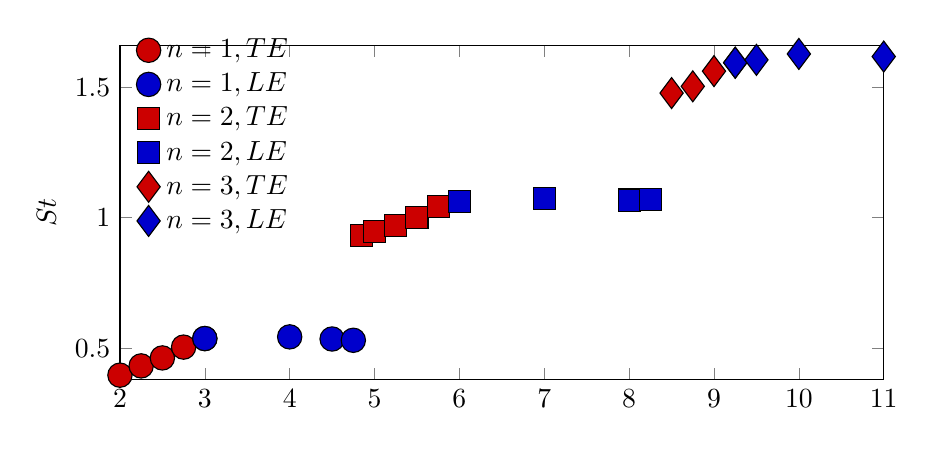
\begin{tikzpicture}



\begin{axis}[%
%width=4.3cm,
%height=3.5cm,
width=0.8\textwidth,
height=0.35\textwidth,
scale only axis,
%grid=both,
%axis lines=middle,
xmin=2,
xmax=11,
ymin=0.38,
ymax=1.66,
%xtick={2, 3, 4, 5, 6, 7, 8, 9, 10, 11},
%ytick={0.4, 0.6, 0.8, 1, 1.2, 1.4, 1.6, 1.8},
%xlabel style={font=\color{white!15!black}},
xlabel={\AR},
ylabel={$St$},
%ymin=0,
%ymax=200,
axis background/.style={fill=white},
legend style={at={(0.01,0.73)}, anchor=west, legend cell align=left, align=left, fill=none, draw=none}
]

\addplot [color=black,only marks,mark=*,mark options={scale=2.2,black,fill=red!80!black}]
  table[row sep=crcr]{%
2       0.396741726829078\\
2.25    0.432248406188668\\
2.5     0.462793383468913\\
2.75    0.504214143890634\\
3       0.536994008053543\\
};
\addlegendentry{$n=1,TE$}

\addplot [color=black,only marks,mark=*,mark options={scale=2.2,black,fill=blue!80!black}]
  table[row sep=crcr]{%
3       0.536994008053543\\
4       0.543439544221324\\
4.5     0.535298051494477\\
4.75    0.530324957725253\\
};
\addlegendentry{$n=1,LE$}


\addplot [color=black,only marks,mark=square*,mark options={scale=2,black,fill=red!80!black}]
  table[row sep=crcr]{%
4.85    0.930407996044941\\
5       0.947349623285183\\
5.25    0.971304878725648\\
5.5     1.000378564453700\\
5.75    1.041747167637721\\
6       1.062464533558995\\
};
\addlegendentry{$n=2,TE$}

\addplot [color=black,only marks,mark=square*,mark options={scale=2,black,fill=blue!80!black}]
  table[row sep=crcr]{%
6       1.062464533558995\\
7       1.073230579537877\\
8       1.067458930414985\\
8.25    1.070000000000000\\
};
\addlegendentry{$n=2,LE$}


\addplot [color=black,only marks,mark=diamond*,mark options={scale=2.8,black,fill=red!80!black}]
  table[row sep=crcr]{%
8.5     1.477258532919061\\
8.75    1.503123920971757\\
9       1.561211928154617\\
9.25    1.593577708455838\\    
};
\addlegendentry{$n=3,TE$}

\addplot [color=black,only marks,mark=diamond*,mark options={scale=2.8,black,fill=blue!80!black}]
  table[row sep=crcr]{%
9.25    1.593577708455838\\    
9.5     1.604355188881951\\
10      1.627228310690177\\
11      1.617135083478177\\
};
\addlegendentry{$n=3,LE$}



%\addplot [color=black,solid,mark=square*,mark options={scale=0.9,black,fill=red!80!black}]
%  table[row sep=crcr]{%
%3       0.609743754434522\\
%4       0.774727821194389\\
%5       0.942866305443131\\
%6       1.100079139112736\\
%7       1.245663824885169\\
%8       1.400191666484032\\
%9       1.546133959599630\\
%10      1.685632118301302\\
%11      1.822225132985195\\
%};



\end{axis}


\end{tikzpicture}%

   \caption{Dependence of $St_L$ on $\AR$ at $Re=400$. Figure adapted from \cite{chiarini-quadrio-auteri-2022}.}
   \label{fig:StLAR}
\end{figure}
%
This stepwise change of $St_L$ is related to the number $n$ of LE vortices that are simultaneously accommodated along the lateral sides of the cylinder, being for example $n=1$ for $\AR=4$, $n=2$ for $\AR=7$ and $n=3$ for $\AR=9$. \cite{chiarini-quadrio-auteri-2022} observed that two different regimes are possible depending on the relative phase between the LE and TE vortices and on the prevalence of either shedding. When the LE vortices dominate the shedding frequency locks to the passing frequency of the LE over the TE and $St \approx n U_c$, where $n$ is the number of LE vortices present simultaneously over the sides of the cylinder and $U_c \approx 0.55 U_\infty$ is the mean convection velocity of the LE vortices \citep[see also][]{mills-sheridan-hourigan-2002,tan-thompson-hourigan-2004}. In contrast, when the TE vortices dominate the flow matches the frequency of elongated bodies with same $\AR$, but rounded LE that does not produce flow separation. Using dynamic mode decomposition, \cite{zhang-etal-2023} observed that the feedback mechanism at $Re = 1000$ changes with $\AR$. For small $\AR$, the feedback loop encompasses the whole separation region and the flow is controlled by the impinging shear-layer instability; for larger $\AR$, the feedback loop covers the entire chord of the cylinder and the flow is controlled by the leading-edge vortex shedding instability.
  
The presence of different regimes and LE/TE vortex interactions hints for the existence of different secondary instabilities and thus different routes to turbulence. To the best of our knowledge, however, a complete picture is still missing and little is known about the secondary instability of the flow past elongated rectangular cylinders with $\AR>1$. It is well established that the flow past a square cylinder ($\AR=1$) undergoes the same sequence of bifurcations mentioned for the circular cylinder case, albeit the primary and secondary instabilities occur at a slightly lower Reynolds number \citep[see for example][]{jiang-cheng-2018,blackburn-sheard-2010}. Indeed, \cite{robichaux-balachandar-vanka-1999}, \cite{blackburn-lopez-2003}, \cite{sheard-fitzgerald-ryan-2009}, \cite{blackburn-sheard-2010} found via Floquet stability analysis that the flow becomes $3D$ due to mode $A$ at $Re \approx 165$, and that modes $B$ and $S$ become unstable only at larger $Re$. By means of 3D Direct Numerical Simulations (DNS), \cite{sheard-fitzgerald-ryan-2009} and \cite{jiang-cheng-an-2018} discussed the saturation effect of the nonlinear terms on the growth of the different modes. \cite{sheard-fitzgerald-ryan-2009} found that the appearance of both modes $A$ and $B$ is due to a supercritical bifurcation. However, \cite{jiang-cheng-an-2018} remarked that, unlike the circular cylinder case \citep{henderson-1997}, the instability of mode A is subcritical; they explained the discrepancy with the results of \cite{sheard-fitzgerald-ryan-2009} with the small computational domain adopted in the latter study. \cite{sheard-fitzgerald-ryan-2009} and \cite{sheard-2011} studied how the angle of incidence affects the unstable modes: mode $A$ is the most unstable one at small and large incidences, while a subharmonic mode, called $C$, is the most unstable at intermediate angles. \cite{choi-yang-2014} considered the flow past rectangular cylinder with $\AR \le 1$, ranging from a flat plate normal to the flow ($\AR \rightarrow 0$) to a square cylinder ($\AR=1$). They found that when reducing $\AR$ both modes $A$ and $B$ stabilise and that new modes A2 and QP2 of synchronous and quasi periodic nature become unstable \citep[see also][]{thompson-etal-2006}. \cite{chaurasia-thompson-2011} and \cite{huang-etal-2017} studied the flow past a semi-indefinite plate of finite thickness, i.e. a rectangular cylinder with $\AR \rightarrow \infty$. The found that the vortices that arise from the LE shear layer due to an induced Kelvin--Helmholtz instability become unstable to subharmonic 3D perturbations at $Re \approx 380$. Despite these works, however, almost no information is available for the secondary bifurcation of the flow past elongated rectangular cylinders with $1 < \AR < \infty$. In a recent work \citep{chiarini-quadrio-auteri-2022d}, we have considered the specific $\AR=5$ ($n=2$ regime dominated by the TE vortex shedding) that defines the BARC benchmark, and found that the secondary instability is due to the QS mode which is of quasi subharmonic nature. Specifically, we found that the wavemaker \citep{monkewitz-huerre-chomaz-1993} of this instability is localised in the region over the longitudinal sides of the cylinder, and that the instability is triggered by the mutual inviscid interaction of the vortices generated by the LE shear layer. It is thus clear that a complete characterisation of how the different flow regimes and LE/TE vortex interaction influence the secondary instability of the flow past rectangular cylinder with $\AR>1$ and thus its route to turbulence is lacking.
    
The aim of this work is to do a step forward in this direction. We aim to fill the gap and characterise the secondary bifurcation of the flow past rectangular cylinders with $1 \le \AR \le 9$ by means of both stability analysis and fully nonlinear 3D DNS. In this work, besides characterising how the different LE/TE vortex interactions influence the bifurcation scenario, we will also provide insights on the triggering mechanism of mode $A$. As shown in the following, indeed, mode $A$ is found only in the regimes dominated by the TE vortices. 
  
The remainder of the work is structured as follows ...

\section{Mathematical formulation and numerical methods}
\label{sec:methods}

\subsection{Flow configuration}
The incompressible flow past rectangular cylinders with aspect ratio $\AR=L/D$, where $L$ and $D$ indicate their length and thickness, is considered. A Cartesian coordinate system centred at the LE of the cylinders is used. The $x$ direction is aligned with the free-stream flow direction, and $y$ denotes the cross-stream direction. When present, $z$ is the spanwise direction. The cylinders are placed in a uniform flow with velocity $\bm{U}=U_\infty\hat{\bm{e}}_x$. The Reynolds number depends on the incoming flow and on the cylinder thickness, and is defined as $Re= U_\infty D /\nu$, where $\nu$ is the kinematic viscosity. The flow is governed by the incompressible Navier--Stokes equations, i.e.
%

\begin{equation}
\begin{aligned}
\frac{\partial U}{\partial t} + \bm{U} \cdot \bm{\nabla}\bm{U} + \bm{\nabla} P - \frac{1}{Re} \nabla^2 \bm{U} & = \bm{0} \\
\bm{\nabla} \cdot \bm{U} & = 0
\end{aligned}
\label{eq:NSequations}
\end{equation}
%
where $\bm{U}$ is the velocity vector with components $\bm{U}=(U,V,W)$ and $P$ is the reduced pressure. No-slip and no-penetration boundary conditions are imposed at the cylinder side, while undisturbed velocity is enforced at the inlet and at the farfield. At the outlet convective boundary conditions
% 
\begin{equation*}
P \bm{n} - \frac{1}{Re} \bm{\nabla} \bm{U} \cdot \bm{n} = \bm{0}
\end{equation*}
%
are used. Periodic boundary conditions are used in the spanwise direction to account for homogeneity.

\subsection{Floquet analysis}

Floquet theory is used to study the linear stability of 2D time-periodic base flows to three-dimensional perturbations. The flow field $\{\bm{U},P\}$ is written as the sum of the a 2D periodic base flow $\{\bm{U}_b,P_b\}$ and an unsteady 3D perturbation of small amplitude $\epsilon$:
\begin{equation}
\{\bm{U},P\}(x,y,z,t) = \{\bm{U}_b,P_b\}(x,y,t) + \epsilon \int_{-\infty}^{\infty} \{\bm{u},p\}(x,y,\beta,t) \text{e}^{i \beta z} \text{d} \beta;
\end{equation}
here $i$ is the imaginary unit, $\bm{u}$ and $p$ indicate the Fourier transform of the velocity and pressure perturbations in the homogeneous $z$ direction and $\beta$ is the corresponding wavenumber.

Introducing this decomposition in \ref{eq:NSequations} the governing equations for the base flow are obtained at order $\epsilon^0$, that are the two-dimensional incompressible Navier--Stokes equations, while the eigenproblem describing the evolution equation for the perturbations are obtained at order $\epsilon^1$. They are the linearised Navier--Stokes equations (LNSEs) that for each $\beta$ read:
%
\begin{equation}
\begin{aligned}
\frac{\partial \bm{u}}{\partial t} + \mathcal{L}_\beta\{\bm{U}_b,Re\}\bm{u} + \bm{\nabla}_\beta p & = \bm{0} \\
\bm{\nabla}_\beta \cdot \bm{u} & = 0
\end{aligned}
\label{eq:LNSEs}
\end{equation}
%
where $\bm{\nabla}_\beta \equiv (\partial / \partial x,\partial / \partial y, i\beta)$ is the Fourier-transformed gradient operator and $\mathcal{L}_\beta$ is the Fourier-transformed linearised Navier--Stokes operator:
%
\begin{equation}
\mathcal{L}_\beta\{\bm{U}_b,Re\}\bm{u}=\bm{U}_b \cdot \bm{\nabla}_\beta \bm{u} + \bm{u} \cdot \bm{\nabla}_\beta \bm{U}_b - \frac{1}{Re} \nabla^2_\beta \bm{u},
\end{equation}
%
where $\nabla^2_\beta \equiv \nabla_\beta \cdot \nabla_\beta$ is the Fourier-transformed Laplacian operator. Following the Floquet theory we further decompose the perturbation field into:
%
\begin{equation}
\{\bm{u},p\}(x,y,\beta,t) = \{\hat{\bm{u}},\hat{p}\}(x,y,\beta,t) \text{e}^{\sigma t}
\end{equation}
%
where $\sigma$ is the Floquet exponent and $\{ \hat{\bm{u}},\hat{p} \}$ is the associated Floquet mode, that has the same periodicity as the base flow. The stability of the system is determined by the sign of the real part $\Re(\sigma)$ of the Floquet exponent, or equivalently, by the modulus of the Floquet multiplier $\mu = e^{\sigma T}$. If all $\Re(\sigma)<0$, or $|\mu<1|$, the system is stable and the perturbations decay. If one exponent exist with $\Re(\sigma)>0$, or $|\mu>1|$ the perturbation grows exponentially; if $\beta \neq 0$ the flow becomes three-dimensional.

\subsection{Computational details}

In the present work we use two distinct numerical methods. The stability analysis is carried out using a numerical code based on finite elements and implemented in the non-commercial software FreeFem++ \citep{hecht-2012}; see \cite{chiarini-quadrio-auteri-2022d} and \cite{chiarini-nastro-2025} for details. The 3D fully non linear simulations are instead carried out with an in-house solver based on finite differences, which has been already used to study the flow past 2D and 3D bluff bodies in both the laminar and turbulent regimes \citep{chiarini-quadrio-auteri-2022d,chiarini-boujo-2024,chiarini-etal-2022}.

The 2D time-periodic base flows $\{\bm{U}_b,P_b\}$ are evaluated by integrating in time the two-dimensional discretised version of the Navier--Stokes equations \ref{eq:NSequations}. The time integration employs an explicit thir-order, low-storage Runge--Kutta method for the non-linear term, combined with an implicity second-order Crank--Nicolson scheme for the linear terms \cite{rai-moin-1991}. The non-commercial, finite-element software FreeFem++ is employed to discretise the equations. Triangular quadratic elements and linear elements are used for the velocity vector and the pressure to satisfy the LBB condition \citep{brezzi-1974}. The BoostConv algorithm \citep{citro-etal-2017} accelerates the convergence of the simulations to the periodic limit cycle; for all cases the base flow is verified to satisfy the requires spatio-temporal symmetries 
\begin{equation}
\{U_b,V_b,P_b\}(x,y,z,t) = \{U_b,-V_b,P_b\}(x,-y,z,t+T/2)
\end{equation}
up to a threshold of $10^{-10}$. The computational domain extends for $-25 D\le x \le 60 D$ in the stremwise direction and for $-40 D \le y \le 40 D $ in the cross-stream direction, leading to $L_x=85D$ and $L_y=80D$. A symmetric grid with respect to the $x$ axis is used to avoid introducing spurious asymmetries in the flow. The number of triangles slightly changes with $\AR$, from a minimum of $8 \times 10^4$ to a maximum of $18 \times 10^4$, and are distributed in order to properly refine the area close to the cylinders and the wake region.

The numerical method used for the Floquet analysis resembles that used by other authors \citep[see for example][]{barkley-henderson-1996}. The Floquet multipliers $\mu_\beta$ and the Floquet modes $\hat{\bm{u}}_\beta(t_0)$ at time $t_0$ of the operator $\mathcal{L}_\beta$ are the eigenvalues and eigenvectors of the linearised Poincarè map $\mathcal{P}_\beta$ that links the velocity perturbation $\bm{u}_\beta(t_0)$ with its evolution after one period, i.e.
%
\begin{equation}
\bm{u}_\beta(t_0+T) = \mathcal{P}_\beta \bm{u}_k(t_0).
\end{equation}
%
The eigenvalues of $\mathcal{P}_\beta$ with larger modulus and the associated eigenvectors have been computed with the Arnoldi method \citep{saad-2011}. The action of $\mathcal{P}_\beta$ on the initial perturbation $\bm{u}_\beta(t_0)$ is obtained integrating in time the LNSEs (equation \ref{eq:LNSEs}) from $t_0$ to $t_0+T$, using the same numerical scheme used for the computation of the base flow. The Gram-Schimdt algorithm is used for the eigenvectors orthogonalisation and all the computed modes are normalised using their total kinetic energy. During the integration of the LNSEs, the base flow is evaluated at each time step by the Fourier interpolation of 100 instantaneous fields stores equispaced in time over one period T.

The 3D Direct Numerical Simulations have been carried out using a numerical code introduced by \cite{luchini-2013}. It integrates in time the three-dimensional Navier--Stokes equations written in primitive variables on a staggered grid using finite-differences in the three directions. The governing equations are advanced in time using a fractional time-stepping method with a third-order Runge-Kutta scheme. The Poisson equation for the pressure is solved using an iterative SOR algorithm. The presence of the cylinder is dealt with a second-order implicit immersed-boundary method \citep{luchini-etal-2025}. For these simulations the computational domain has size $L_x=XXD$, $L_y=XXD$ and $L_z=2\pi D$. The number of points slightly changes with $\AR$, being $(N_x,N_y,N_z) = (XX,XX,XX)$ for $\AR \in (1,3)$, $(N_x,N_y,N_z)=(XX,XX,XX)$ for $\AR =4.5$ and$(N_x,N_y,N_z)=(1040,570,200)$ for $\AR=5.5 $ and $\AR=7$ for a total of about 120 millions points. Their distribution is homogeneous in the spanwise direction, whereas a geometric progression is used the streamwise and vertical directions to properly refine the grid near the cylinders' corners and in the wake region. For all cases the cell size in correspondence of the corners is $\Delta x = \Delta y \approx 0.005D$. All the simulations are advanced in time using a variable timestep to enforce that the Courant–Friedrichs–Lewy number is below unity. 

Hereinafter, if not otherwise indicated, all variables are in dimensionless form with $D$ as length scale, $U_\infty$ as velocity scale and $D/U_\infty$ as time scale.

%\section{What we can do}

\subsection{Strouhal-Reynolds-AR}

It would be interesting to parametrise the $St-Re$ dependence using $\AR$ as a parameter. This would provide a clear visualisation of the successive bifurcations the flow experiences.

\subsection{Neutral curves}

For the 3D bifurcations it would be more effective to draw the neutral curves in the $\beta-Re$ parameter space.


\subsection{Supercritical versus Subcritical bifurcations}

We can assess which is the nature of the bifurcations the flow experiences. For example, we can follow the approach described by Henderson \& Barkley (1996) for the pitchfork bifurcations; see also Henderson (1997).

To assess whether the bifurcation is subcritical or supercritical, we have to look at the influence of the nonlinearity for $Re \rightarrow Re_c$. We now focus on the pitchfork bifurcations. The normal form for a pitchfork bifurcation of a discrete-time dynamical system is
%
\begin{equation}
  A_{n+1} = \mu A_n + \alpha_1 A_n^3 + O(A_n^5)
\end{equation}
%
where $A_n$ corresponds to the real amplitude of the bifurcating flow at period $n$ and $\alpha_1$ is the Landau constant. When $\alpha_1<0$ the instability is a supercritical bifurcation. When $\alpha_1>0$, the instability is a subcritical bifurcation. In this case the transition is discontinuous and hysteretic.

We have to perform direct numerical simulations at $Re \approx Re_c$ using the full $2D$ nonlinear Navier--Stokes equations. Indeed, the most precise and direct way to analyse the nonlinear growth of the critical mode is to follow the evolution of initial conditions of the form $\bm{U}_b + \bm{u}_c$, where $\bm{u}_c$ is the Floquet mode at criticality. Moreover, since the initial conditions is characterised by a single wavenumber $\beta_c$, it is clear that due to the properties of the Navier--Stokes equations it is sufficient to retain in the NS equations only those modes with $\beta = m \beta_c$, where $m$ is an integer. This allows to not perform an actual 3D simulation.
The amplitude $A_n$ at this point may be simply considered as
%
\begin{equation}
  A_n \equiv =  \left( \frac{1}{\Omega U_\infty^2} \int_{\Omega} |\bm{u}^n_c|^2 \text{d} \Omega \right)^{1/2}
\end{equation}
%
where $\Omega$ is the area of the computational domain, and $\bm{u}^n_c$ is the Fourier coefficient of the velocity field at period $n$ and wavenumber $\beta_c$. In doing this, we can then plot $A_n$ as a function of the iteration and then evaluate the value of $\alpha_1$ as
%
\begin{equation}
  \alpha_1 \approx \frac{ A_{n+1} - \mu A_n}{A_n^3}.
\end{equation}
%

Clearly, in the case where the bifurcation is two-dimensional the approach is rather easy. In this case, indeed, $\beta_c = 0$. For three-dimensional bifurcations, instead, the situation is more complex and we should choose in somehow the number of mode to include in the 3D non linear simulations such that $m\le M$.

In the case the bifurcations are subcritical we should study the bi-stability interval.


For the specific case of the circular cylinder mode A is subcritcal, while mode B is supercritical.


Another possible approach to study the non linear effect is to carry out DNS close to the onset of the bifurcation.

\subsubsection{3D pitchfork}

After the flow bifurcation we can write
%
\begin{equation}
  \bm{U}(\bm{x},t) = U(t) \bm{\phi}_0(\bm{x},t) + A(t) \bm{\phi}_1(\bm{x},t).
\end{equation}
%
The idea is to study how non linearity influences the values of $U$ and $A$ in time. This would allow us to understand whether the bifurcations is subcritical or supercritical.

The idea is to decompose the velocity and pressure field using a Fourier decomposition, i.e.
%
\begin{equation}
  \bm{U}(\bm{x},t) = \sum_{j=0}^M \hat{\bm{u}}_j e^{i j \beta_c z} = \hat{\bm{u}}_0(\bm{x},t) + \hat{\bm{u}}_1(\bm{x},t) e^{i \beta_c z}+
                     \sum_{j=2}^M \hat{\bm{u}}_j e^{i j \beta_c z} 
\end{equation}
%
where $\beta_c$ is the critical wavenumber (result of the Floquet analysis). $\hat{\bm{u}}_0(\bm{x},t)$ denotes the spatial average and describes the evolution of the two-dimensional base flow. $\hat{\bm{u}}_1(\bm{x},t)$ denotes the coefficient associated with the Fourier mode having $\beta = \beta_c$.

At this point, we use as initial condition 
%
\begin{equation}
  \hat{\bm{u}}_0(\bm{x},t_n) = \bm{U}_b(\bm{x},0)
\end{equation}
%
where $\bm{U}_b$ denotes the saturated base flow evaluated with the non linear 2D Navier--Stokes equations, and
%
\begin{equation}
  \hat{\bm{u}}_1(\bm{x},t_n) = \bm{u}_{Fl}(\bm{x},0)
\end{equation}
%
where $\bm{u}_{Fl}$ denotes the most unstable Floquet mode.
We then integrate this initial condition using the complete, 3D and non linear Navier--Stokes equations to detect the effect of the non linearity on the bifurcation. In particular, we track the values of $U_n$ and $A_n$ as
%
\begin{equation}
  |U_n|^2 = \frac{1}{\Omega U_\infty^2} \int_{\Omega} | \hat{\bm{u}}_0(\bm{x},t_n |^1 \text{d}\Omega
\end{equation}
%
and
\begin{equation}
  |A_n|^2 = \frac{1}{\Omega U_\infty^2} \int_{\Omega} | \hat{\bm{u}}_1(\bm{x},t_n |^1 \text{d}\Omega
\end{equation}
%
where $A_n=A(t_n)$ and $t_n$ is such that $C_\ell(t_n) = 0$. Note that in doing this it is possible that the period of the oscillation actually changes due to the influence of the nonlinearity.

This allows as to evaluate whether the bifurcation is supercritical or subcritical. In fact, the normal form for a picthfork bifurcation is
%
\begin{equation}
  A_{n+1} = \left( \mu_1 + \sum_j \alpha_{ij}A_n^{2j} \right) A_n
\end{equation}
%
and the value of $\alpha_{11}$ determines whether the bifurcation is supercritical ($\alpha_{11}<0$) or subcritical ($\alpha_{11}>0$). Note that $\mu_1 = 1 + \mu'\epsilon$ where $\mu' = \text{d}\mu/\text{d}\epsilon$ and $\epsilon = (Re - Re_c)/Re_c$ is the small parameter.

At this point, by comparing the found value of $A_{n}$ with the normal form truncated at $j=1$ one may determine the value of $\alpha_{11}$. For a supercritical bifurcation then it is easy to evaluate the saturated state. Indeed in the saturated case $A_{n+1}=A_n$ and $\mu_1 + \alpha_{11}A_n^2 = 1$. This means that $\mu' \epsilon + \alpha_{11}A_n^2=0$ from which
%
\begin{equation}
  A_n^2 = - \frac{ \mu' \epsilon}{\alpha_{11}}
\end{equation}
%
where the values of $\mu'$ and $\alpha_{11}$ can be estimated from the DNS data.

In the case of a supercritical bifurcation the situation is more convoluted. Indeed, to assess the saturated state we need an additional term if our expansion. Thus we stop at $j=2$. This means that in this case
%
\begin{equation}
  A_{n+1} = \left( \mu_1 + \alpha_{11}A_n^2 + \alpha_{12} A_n^4 \right) A_n,
\end{equation}
%
where again $\alpha_{12}$ may be estimated from the data.
As such the saturated state reads $\mu_1 + \alpha_{11} A_n^2 + \alpha_{12} A_n^4 = 1$, meaning that $\mu' \epsilon + \alpha_{11} A_n^2 + \alpha_{12} A_n^4 = 0$ that leads to
%
\begin{equation}
  |A|^2 = \frac{\alpha_{11}}{2 \alpha_{12}} \pm \left( \frac{\alpha_{11}^2}{4 \alpha_{12}^2} - \frac{\mu_1' \epsilon}{\alpha_{12}} \right)^{1/2}.
\end{equation}

\subsubsection{2D Pitchfork}

For the two-dimensional case the situation is rather different. In this case we do not use a Fourier series. Instead, we write the velocity field as
%
\begin{equation}
\bm{U}(\bm{x},t) = \bm{U}_b(\bm{x},t) + \bm{u}'(\bm{x},t)
\end{equation}
%
where $\bm{U}_b$ is the symmetric base flow obtained after stabilising the flow with the BoostConv algorithm, and $\bm{u}'(\bm{x,t})$ is instead the nonlinear perturbation that drives the flow towards the slanted configuration.

The idea, therefore, is to carry out a 2D simulation using the non linear Navier--Stokes equations using
%
\begin{equation}
  \bm{u}'(\bm{x},t_n) = A_0 \bm{u}_{Fl}(\bm{x},0)
\end{equation}
%
as initial condition. At this point, we track in time $A_n=A(t_n)$ (in this case the period does not change), and assess whether the bifurcation is either supercritical or subcritical by looking at $\alpha_{11}$ that appears in the normal form
%
\begin{equation}
 A_{n+1} = \left( \mu + \alpha_{11} A_n^2 \right) A_n.
\end{equation}
%
In this case we can also do other considerations regarding the shape of the saturated stated etc; see Jallas et al (2017).


\subsection{Wavemaker}

It is worth localising the wavemaker for the different instabilities that we detect. Indeed, this is useful for control purposes, as it localises the flow region where we should modify things to interact with the flow instability. We can use two different approaches. On the one side, we can look at the structural sensitivity (Giannetti et al, 2010). 

A different apprach would be to perform Floquet stability analyses on small portions of the complete domain, similar to what done by Barkley (2005), in the context of the circular cylinder. The idea is the following. We first compute the base flow in the complete domain, by imposing the usual boundary conditions. Then, we extract portions of the base flow in some subdomains, directly from that computed on the full domain. At this point we perform Floquet analysis on these subdomains. The base flow is "exact" whatever the subdomain we consider. The mode will change as we will impose boundary conditions in different points, depending on the size of the considered subdomain: for each subdomain we impose $\bm{u}=0$ at all the boundaries, but at the outlet where we impose homoegeneous Neumann conditions. The idea is to use this approach to further show that the triggering mechanism of the QS mode is embedded in over the side of the cylinder. More in detail, the idea is to show that for $\AR=5.5$ modes $QS$ and $A$ coexist, as one is a unstable mode of the LE vortices, while the other is an unstable mode of the wake. In this way, by selecting properly the subdomains we can clearly show this effect.


\subsection{$5 \le \AR \le 6$}

In this range of $Re$ the flow first becomes three-dimensional due to the so-called mode A. Then, also mode $QS$ appears. This is perfectly predicted by the linear stability analysis. However, can we say something more on this? For example, are these bifurcations subcritical or supercritical? How the flow moves to mode $QS$? In a gradual way? Can we use POD on 3D DNS to assess which is the amount of energy contained in the two modes? Centre manifold?

Also, it would be nice to derive the amplitude equations for the two modes to see how they interact. See Barkley et al (2000) for the amplitude equations of modes A and B in the case of the circular cylinder. For this it would be necessary to study the book by Golubitsky, volume II.


\subsection{Dependence on the domain size}

It is of great interest also to determine which is the influence of the spanwise size of the computational domain, i.e. the largest wavelength of the perturbation that is allowed in the flow, especially at $Re>Re_{c2}$. We may use $\AR=5.5$ to investigate this effect for $Re>550$, by keeping the grid dsciretisation constant and progressively increasing the number of points in the spanwise direction together with $L_z$.

\subsection{POD, SPOD}

To further characterise the modes at larger $Re$ in the different case we can resort to the POD and SPOD modes. This may be useful to assess how energetic are the different modes as $Re$ increases, and whether the relevance of a certain mode compared to the others becomes more or less relevant.

\subsection{Modes A and B}

Can we use the $\AR$ parameter to discuss the triggering mechanisms of these two modes? Indeed, by simply changing the $\AR$ we find that these modes appear and disappear. This is clearly due to the fact that the way the LE and TE vortices interact changes. Let's try.

\subsection{How to present the results}

We can represent the base flow by looking at the vorticity and at $\kappa = 2S/|\Omega|$ where $S$ is the positive eigenvalue of the strain of rate tensor and $\Omega$ is the vorticity. $\kappa>1$ denotes hyperbolic regions, while $\kappa<1$ regions where the rotation dominates (elliptic regions).

Maybe it would be interesting also to show how the spatial distribution of the eigenvectors change with $\beta$.

\subsection{Energy budget for the modes}

To provide further insight on the physical mechanism that leads to the exponential amplification of the modes (when the linear approximation holds), we can look at the energy budget of the mode itself. This would provide us with information regarding the region where the base flow energises the mode itself, where the transport term dominates, and where the viscous dissipation dominates. The idea is to write the linearised Navier--Stokes equations, i.e.
%
\begin{equation}
  \frac{\partial u_i}{\partial t}  = - U_j \frac{\partial u_i}{\partial x_j} - u_j \frac{\partial U_i}{\partial x_j} - \frac{1}{\rho}\frac{\partial p}{\partial x_i} + \frac{1}{Re} \frac{\partial^2 u_i}{\partial x_j^2}; \ \frac{\partial u_j}{\partial x_j} = 0.
\end{equation}
We recall that since we use the Floquet theory we can write
%
\begin{equation}
  u_i = \tilde{u}_i(x,y,z,t) e^{\sigma t}.
\end{equation}
%
To obtain the energy equation we thus take the LNSE and multiply for $\tilde{u}_i^*$, where the $\cdot^*$ superscript refers to the complex conjugate. Then we take the conjugate of the LNSE and mulitpliy it for $\tilde{u}_i$. Eventually we sum the two equations to obtain the equation for the energy.
It is worth recalling that we use a Fourier expansion in the $z$ direction, such that
%
\begin{equation}
  \tilde{u}_i(x,y,z,t) = \sum \hat{u}_{\beta,i}(x,y,t) e^{i\beta z}:
\end{equation}
%
For simiplicity, hereafter we drop the $\cdot_\beta$ subscript.
Now, we look at the energy equation for each single Fourier mode.

The first equation reads:
%
\begin{equation}
\left( \frac{\partial \tilde{u}_i}{\partial t} + \sigma \tilde{u}_i \right) \tilde{u}^*_i =
- \tilde{u}_j \tilde{u}_i^* \frac{\partial U_i}{\partial x_j} - U_j \frac{\partial \tilde{u}_i}{\partial x_j} \tilde{u}_i^*
- \frac{1}{\rho} \frac{\partial \tilde{p}}{\partial x_i} \tilde{u}_i^* 
+ \frac{1}{Re} \frac{\partial^2 \tilde{u}_i}{\partial x_j^2} \tilde{u}_i^*,
\end{equation}
whle the second equations reads (recall that in our case $U_3=0$:
\begin{equation}
\left( \frac{\partial \tilde{u}_i^*}{\partial t} + \sigma^* \tilde{u}_i^* \right) \tilde{u}_i = 
- \tilde{u}_j^* \tilde{u}_i \frac{\partial U_i}{\partial x_j} - U_j \frac{\partial \tilde{u}_i^*}{\partial x_j} \tilde{u}_i
- \left( \frac{1}{\rho} \frac{\partial \tilde{p}}{\partial x_i} \right)^* \tilde{u}_i + 
\frac{1}{Re} \left( \frac{\partial \tilde{u}_i}{\partial x_j^2} \right)^* \tilde{u}_i
\end{equation}
%
We now sum the two equations and look separately at the different terms. Recall that $\tilde{u}_i^* = \hat{u}_i^* e^{-i\beta z}$.
\begin{itemize}
  \item
  \begin{equation}
    \left( \frac{\partial \tilde{u}_i}{\partial t} + \sigma \tilde{u}_i \right) \tilde{u}_i^* +
    \left( \frac{\partial \tilde{u}_i^*}{\partial t} + \sigma^* \tilde{u}^*_i \right) \tilde{u}_i = 
    \frac{\partial \hat{u}_i \hat{u}^*_i}{\partial t} + ( \sigma^* + \sigma ) \hat{u}_i \hat{u}_i^* = 
    \frac{\partial \hat{u}_i \hat{u}^*_i}{\partial t} + 2 \Re(\sigma) \hat{u}_i \hat{u}_i^* 
  \end{equation}
  \item
  \begin{equation}
    - \tilde{u}_j \tilde{u}_i^* \frac{\partial U_i}{\partial x_j} - 
      \tilde{u}_i \tilde{u}_j^* \frac{\partial U_i}{\partial x_j} = - ( \hat{u}_j \hat{u}_i^* + \hat{u}_i \hat{u}_j^* ) \frac{\partial U_i}{\partial x_j}
  \end{equation}
  \item
  \begin{equation}
    - U_j \frac{\partial \tilde{u}_i}{\partial x_j} \tilde{u}_i^* - U_j \frac{\partial \tilde{u}_i^*}{\partial x_j} \tilde{u}_i = 
    - U_j \frac{\partial \hat{u}_i \hat{u}_i^*}{\partial x_j}
  \end{equation}
  \item
  \begin{equation}
  \begin{gathered}
    - \frac{1}{\rho} \frac{\partial \tilde{p}}{\partial x_i} \tilde{u}_i^* - 
      \frac{1}{\rho} \left( \frac{\partial \tilde{p}}{\partial x_i} \right)^* \tilde{u}_i = 
    - \frac{1}{\rho} \frac{\partial \hat{p} \hat{u}_i^*}{\partial x_i} + \frac{\hat{p}}{\rho} \frac{\partial \hat{u}_i^*}{\partial x_i} - 
    \frac{1}{\rho} \left( \frac{\partial \hat{p}^*}{\partial x_i} \hat{u}_i - i \beta \hat{p}^* \hat{u} \right) = \\
    - \frac{1}{\rho} \frac{\partial \hat{p} \hat{u}_i^*}{\partial x_i} -
      \frac{1}{\rho} \frac{\partial \hat{p}^* \hat{u}_i}{\partial x_i} = 
      - \frac{1}{\rho} \frac{\partial}{\partial x_i} \left(  \hat{p} \hat{u}_i^* + \hat{p}^* \hat{u}_i \right)
  \end{gathered}
  \end{equation}
  \item 
  \begin{equation}
  \begin{gathered}
    \frac{1}{Re} \frac{\partial^2 \tilde{u}_i}{\partial x_j^2} \tilde{u}_i^* +
    \frac{1}{Re} \left( \frac{\partial^2 \tilde{u}_i}{\partial x_j^2} \right)^* \tilde{u}_i = \\
    \frac{1}{Re} \frac{\partial}{\partial x_j} \left( \frac{\partial \tilde{u}_i}{\partial x_j} \right) \tilde{u}_i^* +
    \frac{1}{Re} \left[ \frac{\partial}{\partial x_j} \left( \frac{\partial \hat{u}_i^*}{\partial x_j} \hat{u}_i - \beta^2 \hat{u}_i^* \hat{u}_i \right) \right] = \\
    \frac{1}{Re} \left[ \frac{\partial}{\partial x_j} \left( \frac{\partial \hat{u}_i \hat{u}_i^*}{\partial x_j} \right) \right]
   -\frac{1}{Re} \left( 2 \frac{\partial \hat{u}_i}{\partial x_j} \frac{\partial \hat{u}_i^*}{\partial x_j} + \beta^2 \hat{u}_i^* \hat{u}_i \right)
  \end{gathered}
  \end{equation}
\end{itemize}

Therefore the equation for the energy reads
%
\begin{equation}
\begin{gathered}
\frac{\partial \hat{u}_i \hat{u}_i^*}{\partial t} + 2 \Re(\sigma) \hat{u}_i \hat{u}_i^* = 
- \left( \hat{u}_j \hat{u}_i^* + \hat{u}_i \hat{u}_j^* \right) \frac{\partial U_i}{\partial x_j} -
\frac{\partial}{\partial x_j} \left( U_j \hat{u}_i \hat{u}_i^*\right)  + \\
- \frac{1}{\rho} \frac{\partial}{\partial x_i} \left( \hat{p} \hat{u}_i^* + p^* \hat{u}_i \right) +
\frac{1}{Re} \frac{\partial}{\partial x_j} \left( \frac{ \partial \hat{u}_i \hat{u}_i^*}{\partial x_j} \right) 
- \frac{1}{Re} \left( 2 \frac{\partial \hat{u}_i}{\partial x_j} \frac{\partial \hat{u}_i^*}{\partial x_j} + 2 \beta^2 \hat{u}_i^* \hat{u}_i \right) 
\end{gathered} 
\end{equation}

%
We now average over one period to remove the dependence on $\partial \hat{u}_i \hat{u}_i^*/\partial t$. We thus obtain:
%
\begin{equation}
  \begin{gathered}
  \frac{2 \Re(\sigma)}{T} \int_{t_0}^{t_0+T} \hat{u}_i \hat{u}_i^* \text{d}t = 
 -\frac{1}{T} \int_{t_0}^{t_0+T} \left( \hat{u}_j \hat{u}_i^* + \hat{u}_j^* \hat{u}_i \right) \frac{\partial U_i}{\partial x_j} \text{d} t +\\
 -\frac{1}{T} \int_{t_0}^{t_0+T} U_j \frac{\partial \hat{u}_i \hat{u}_i^*}{\partial x_j} \text{d} t + 
 -\frac{1}{T} \int_{t_0}^{t_0+T} \frac{\partial}{\partial x_i} \left( \hat{p} \hat{u}_i^* + \hat{p}^* \hat{u}_i \right) \text{d}t + \\
 +\frac{1}{T} \int_{t_0}^{t_0+T} \frac{1}{Re} \left[ \frac{\partial}{\partial x_j} \left( \frac{\partial \hat{u}_i^* \hat{u}_i }{\partial x_j} \right) \right] \text{d}t 
 -\frac{1}{T} \int_{t_0}^{t_0+T} \frac{1}{Re} \left( 2 \frac{\partial \hat{u}_i}{\partial x_j} \frac{\partial \hat{u}_i^*}{\partial x_j} + 2 \beta^2 \hat{u}_i^* \hat{u}_i \right) \text{d} t
 \end{gathered}
\end{equation}

To provide further insights on the physical mechanism of the modes we can also look at the budget equation for the enstrophy, which is defined as $\hat{\omega}_i \hat{\omega}_i^*$. We follow a similar approach like for the energy budget. However, in this case we start from the linearised equation for the vorticity, which reads:
%
\begin{equation}
  \frac{\partial \omega_i}{\partial t} + U_j \frac{\partial \omega_i}{\partial x_j} + u_j \frac{\partial \Omega}{\partial x_j} = \Omega_j \frac{\partial u_i}{\partial x_j} + \omega_j \frac{\partial U_i}{\partial x_j} + \frac{1}{Re} \frac{\partial^2 \omega_i}{\partial x_j^2}.
\end{equation}
%
We then follow the same approach as before and eventually obtain (here we use the fact that $\bm{\Omega} = \Omega \hat{\bm{e}}_3$)
%
\begin{equation}
  \begin{gathered}
  \frac{\partial \hat{\omega}_i \hat{\omega}^*_i}{\partial t} + 
  2 \Re(\sigma) \hat{\omega}_i \hat{\omega}_i^* = 
  - \left( \hat{\omega}_i^* \hat{u}_j + \hat{\omega}_i u_j^* \right) \frac{\partial \Omega_i}{\partial x_j} 
  - U_j \frac{\partial \hat{\omega}_i \hat{\omega}_i^* }{\partial x_j}  +
   i \beta \Omega_3 \left( \hat{u}_i \hat{\omega}_{i}^* - \hat{u}_i^* \hat{\omega}_i \right)  + \\
   + \left( \hat{\omega}_i^* \hat{\omega}_j + \hat{\omega}_i \hat{\omega}_j^* \right) \frac{\partial U_i}{\partial x_j} + 
   \frac{1}{Re} \frac{\partial}{\partial x_j} \left( \frac{\partial \hat{\omega}_i \hat{\omega}_i^*}{\partial x_j} \right) -
   \frac{1}{Re} \left( 2 \frac{\partial \hat{\omega}_i}{\partial x_j} \frac{\partial \hat{\omega}^*}{\partial x_j} + 2 \beta^2 \hat{\omega}_i \hat{\omega}^* \right)
  \end{gathered}
\end{equation}
%
As above, we now integrate over one period, i.e. between $t_0$ and $t_0+T$ and obtain
%
\begin{equation}
  \begin{gathered}
  \frac{2 \Re{\sigma}}{T} \int_{t_0}^{t_0+T} \hat{\omega}_i \hat{\omega}_i^* \text{d}t = 
  - \frac{1}{T} \int_{t_0}^{t_0+T} \left( \hat{\omega}_i^* \hat{u}_j + \hat{\omega}_i u_j^* \right) \frac{\partial \Omega_i}{\partial x_j} \text{d}t
  - \frac{1}{T} \int_{t_0}^{t_0+T} U_j \frac{\partial \hat{\omega}_i \hat{\omega}_i^* }{\partial x_j} \text{d} t + \\
  + \frac{1}{T} \int_{t_0}^{t_0+T}    i \beta \Omega_3 \left( \hat{u}_i \hat{\omega}_{i}^* - \hat{u}_i^* \hat{\omega}_i \right)  \text{d} t
  + \frac{1}{T} \int_{t_0}^{t_0+T} \left( \hat{\omega}_i^* \hat{\omega}_j + \hat{\omega}_i \hat{\omega}_j^* \right) \frac{\partial U_i}{\partial x_j} \text{d} t + \\
  + \frac{1}{T} \int_{t_0}^{t_0+T}    \frac{1}{Re} \frac{\partial}{\partial x_j} \left( \frac{\partial \hat{\omega}_i \hat{\omega}_i^*}{\partial x_j} \right) \text{d} t -
  \frac{1}{T} \int_{t_0}^{t_0+T} \frac{1}{Re} \left( 2 \frac{\partial \hat{\omega}_i}{\partial x_j} \frac{\partial \hat{\omega}_i^*}{\partial x_j} + 2 \beta^2 \hat{\omega}_i \hat{\omega}_i^* \right) \text{d} t
  \end{gathered}
\end{equation}
XXX nelle derivate della dissipazione il pedice j indica anche le derivate in z? non sono già contate da beta*beta?XXX

%\section{Results}

%\section{The bifurcation scenario}

We start by looking at the bifurcation scenario, which is shown in figure \ref{}.

\begin{itemize}
  \item Add a figure with $Re$ on the $y$ axis and $\AR$ on the $x$ axis. Add information regarding the primary bifurcation. Add information regarding where we have the flow regime dominated by the TE vortex shedding and by the LE vortex shedding. Add informaiton regarding what is the kind of secondary bifurcation we do expect, by adding also qualitative snapshots of the modes. Here we only show the most unstable mode, and so we do not characterise the secondary instability of the limit cycle. This is also a way to recap the differences in the base flow. 
\end{itemize}


\section{Short bodies}
\label{sec:short}

XX per AR=2 FISSA RE FLUSSO BASE E ALZA RE STABILIT PER VEDERE SE QUI SI STABILIZZA O MENO XX

We begin by examining short bodies with aspect ratios in the range $1 \le \AR <3$, to assess how a modest increase in $\AR$ alters the bifurcation structure and the sequence in which flow modes become unstable, relative to the well-studied $\AR=1$ case. This analysis complements the work of \cite{choi-yang-2014}, who investigated the onset of secondary instabilities for bodies ranging from a flat plate normal to the flow ($\AR \rightarrow 0$) to a square cylinder ($\AR=1$).

\subsection{The base flow}

\begin{figure}
  \centering
  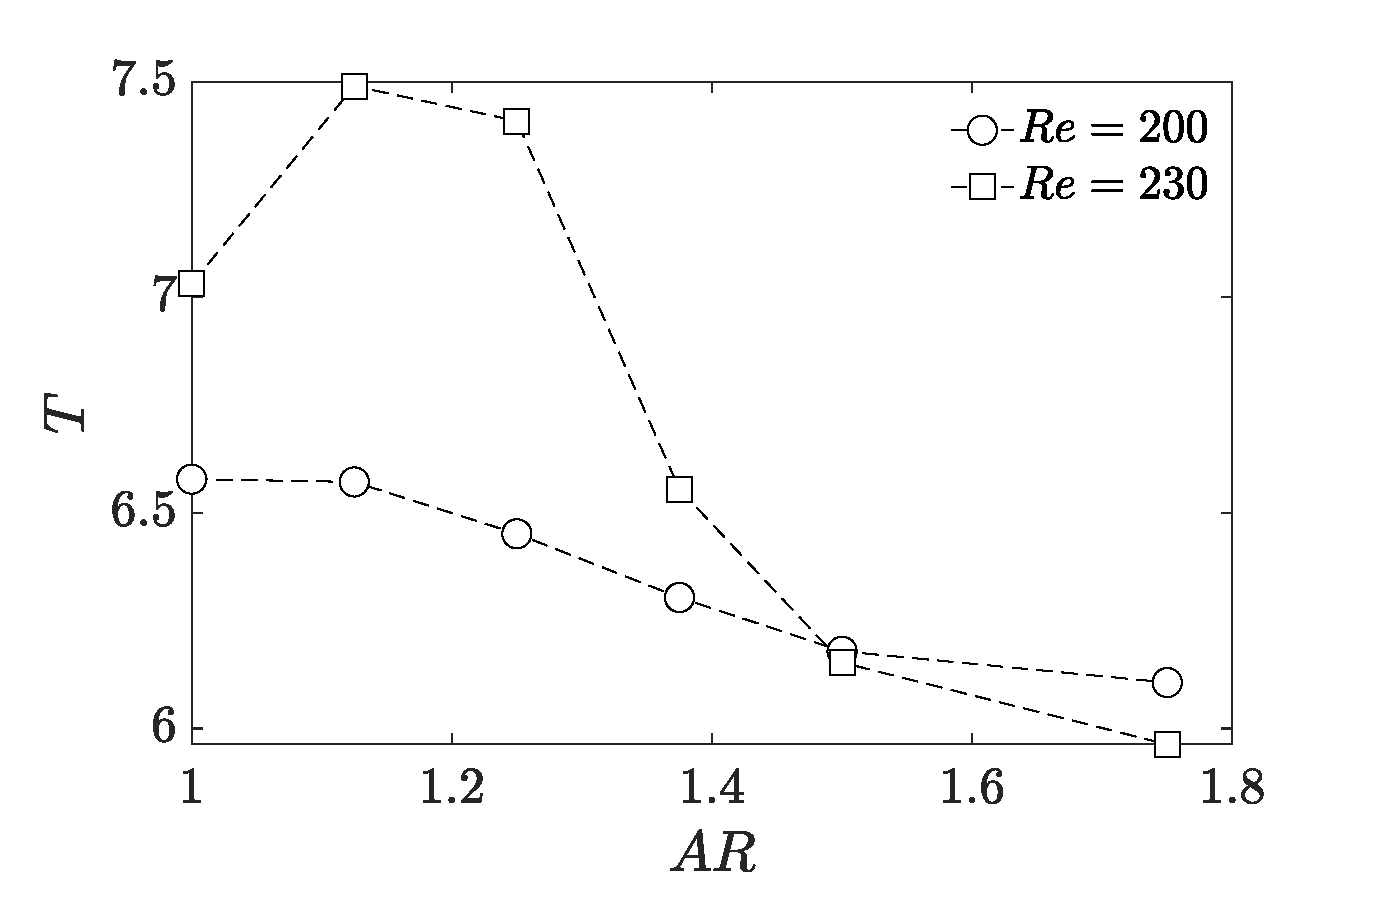
\includegraphics[width=0.49\textwidth]{./fig/AR1s/T_AR.eps}
  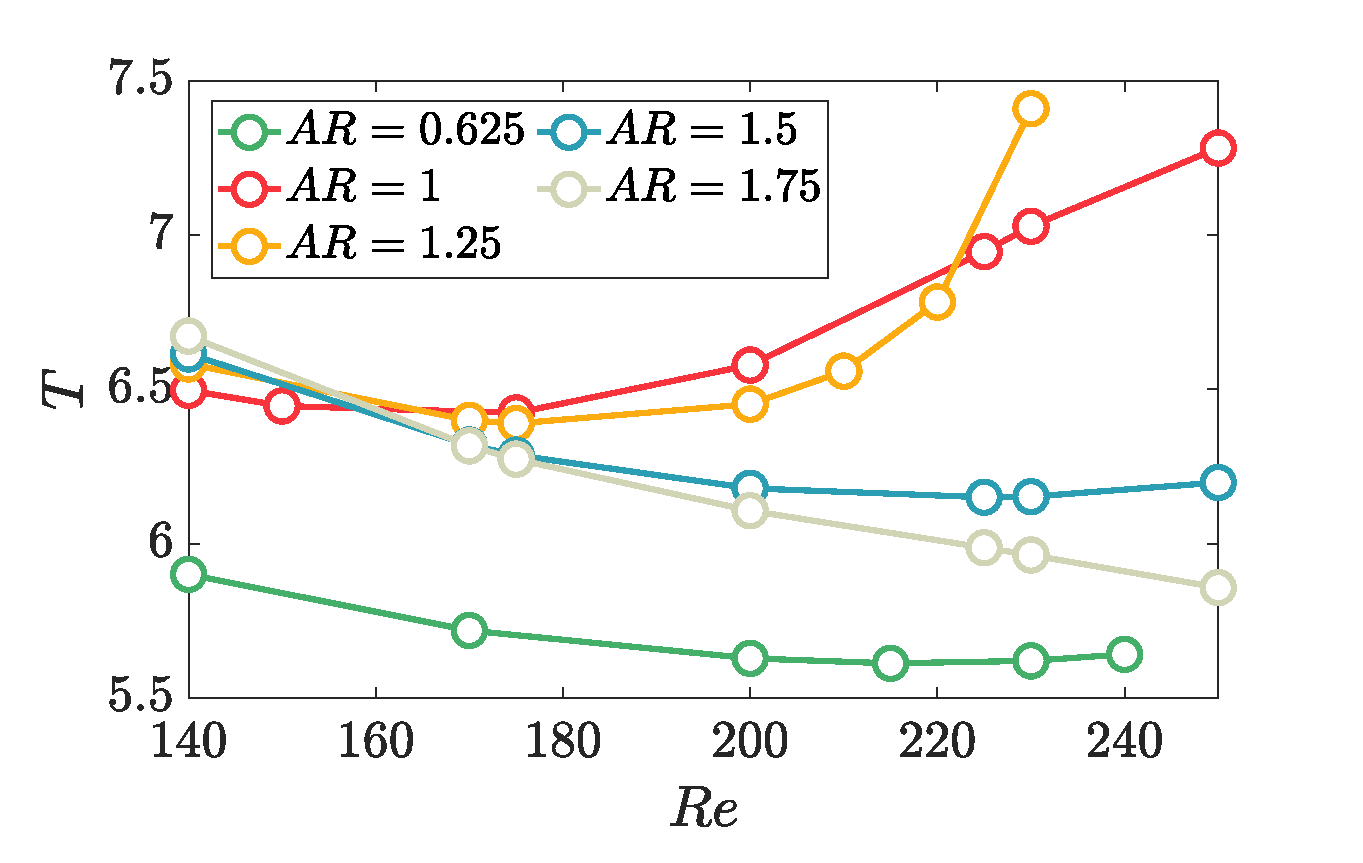
\includegraphics[width=0.49\textwidth]{./fig/AR1s/T_Re.eps}
  \caption{Base-flow period as a function of $\AR$ and $Re$. Left: dependence of $T$ on $Re$ for $1 \le \AR \le 1.75$. Right: dependence of $T$ on $\AR$ for $Re=200$ and $Re=230$. XX MODIFICARE FIGURA USANDO PALLINI PIENI QUANDO RIATTACCA IN MEDIA E VUOTI QUANDO NON RIATTACCA IN MEDIA; AGGIUNGERE CON UN INSET DIPENDENZA DELLA BOLLA DI RICIRCOLO MEDIA CON RE PER ALCUNI CASI PARTICOLARI. XX}
  \label{fig:T_Re_small}
\end{figure}
%

We begin by characterising the influence of aspect ratio $\AR$ and Reynolds number $Re$ on the periodic base flow. Figure \ref{fig:T_Re_small} shows the variation of the base-flow shedding period $T$ with both parameters. In figure \ref{fig:T_Re_small}(b), for $\AR=1.25$, results are not reported beyond $Re=240$, as the two-dimensional base flow loses periodicity near $Re \approx 250$ due to a Neimark–Sacker bifurcation (not shown for brevity).
%
The shedding period exhibits a strong dependence on both $\AR$ and $Re$. For the shortest bodies ($\AR \lessapprox 1$), the period $T$ varies only mildly with $Re$: for example, when $Re$ increases from $140$ to $230$, $T$ increases by approximately $2.2\%$ for $\AR=0.75$, see figure \ref{fig:T_Re_small}(b). In contrast, for intermediate ($1 \lessapprox \AR \lessapprox 1.5$) and longer bodies ($\AR \gtrapprox 1.5$), the variation is more pronounced. Over the same $Re$ range, $T$ increases by $12.6\%$ for $\AR=1.25$, while it decreases by $12.9\%$ for $\AR=3$.
%
When holding $Re$ fixed and varying $\AR$, figure~\ref{fig:T_Re_small}(a) shows that $T$ increases monotonically with $\AR$ for $Re \le 140$. At higher Reynolds numbers, however, $T$ displays a non-monotonic dependence on $\AR$, with a maximum around the intermediate $\AR \approx 1.25$. Interestingly, the dependence of $T$ on both $\AR$ and $Re$ mirrors that of the time-averaged wake recirculation length $\ell_w$ (see the inset in figure \ref{fig:T_Re_small}(v)), measured using the mean streamline defined by $\aver{\Psi_b} = 0$, where the streamfunction $\Psi_b$ satisfies $\bm{\nabla}^2 \Psi_b = - \omega$.

\begin{figure}
  \centering
  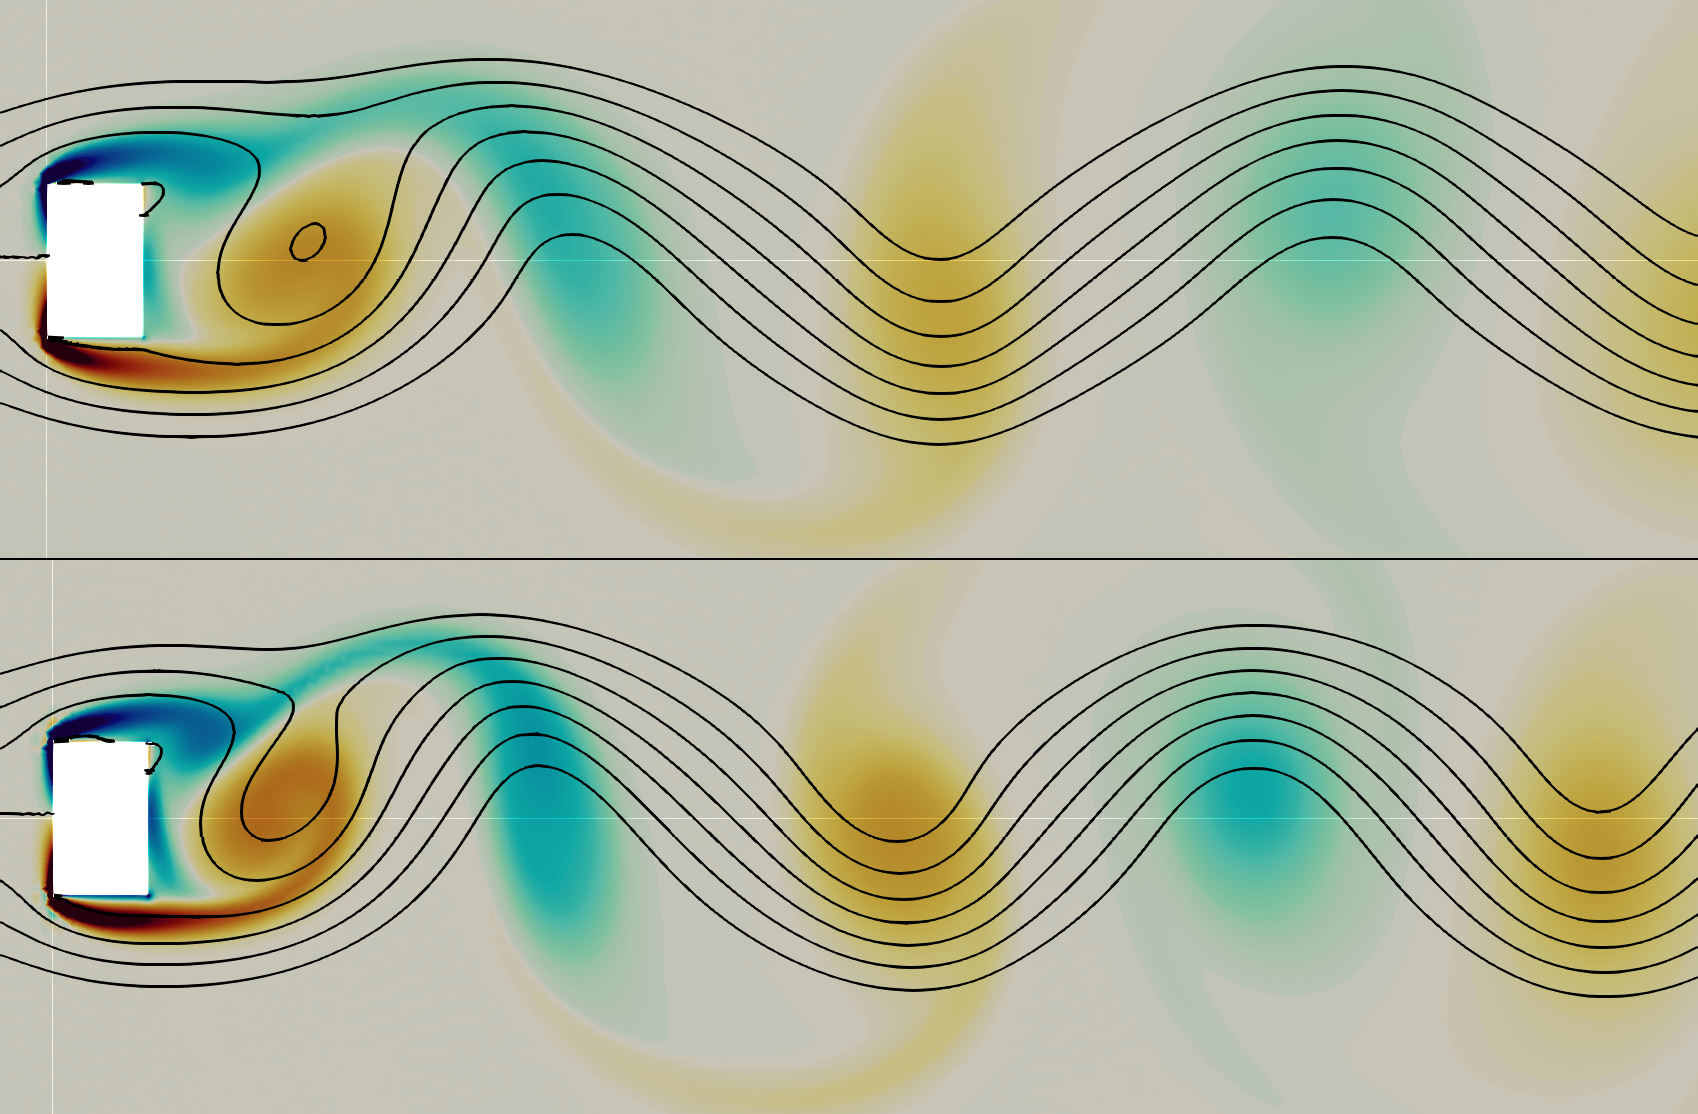
\includegraphics[width=0.49\textwidth]{./fig/AR1s/AR0p625_Re140_Re230_omegaz.png}
  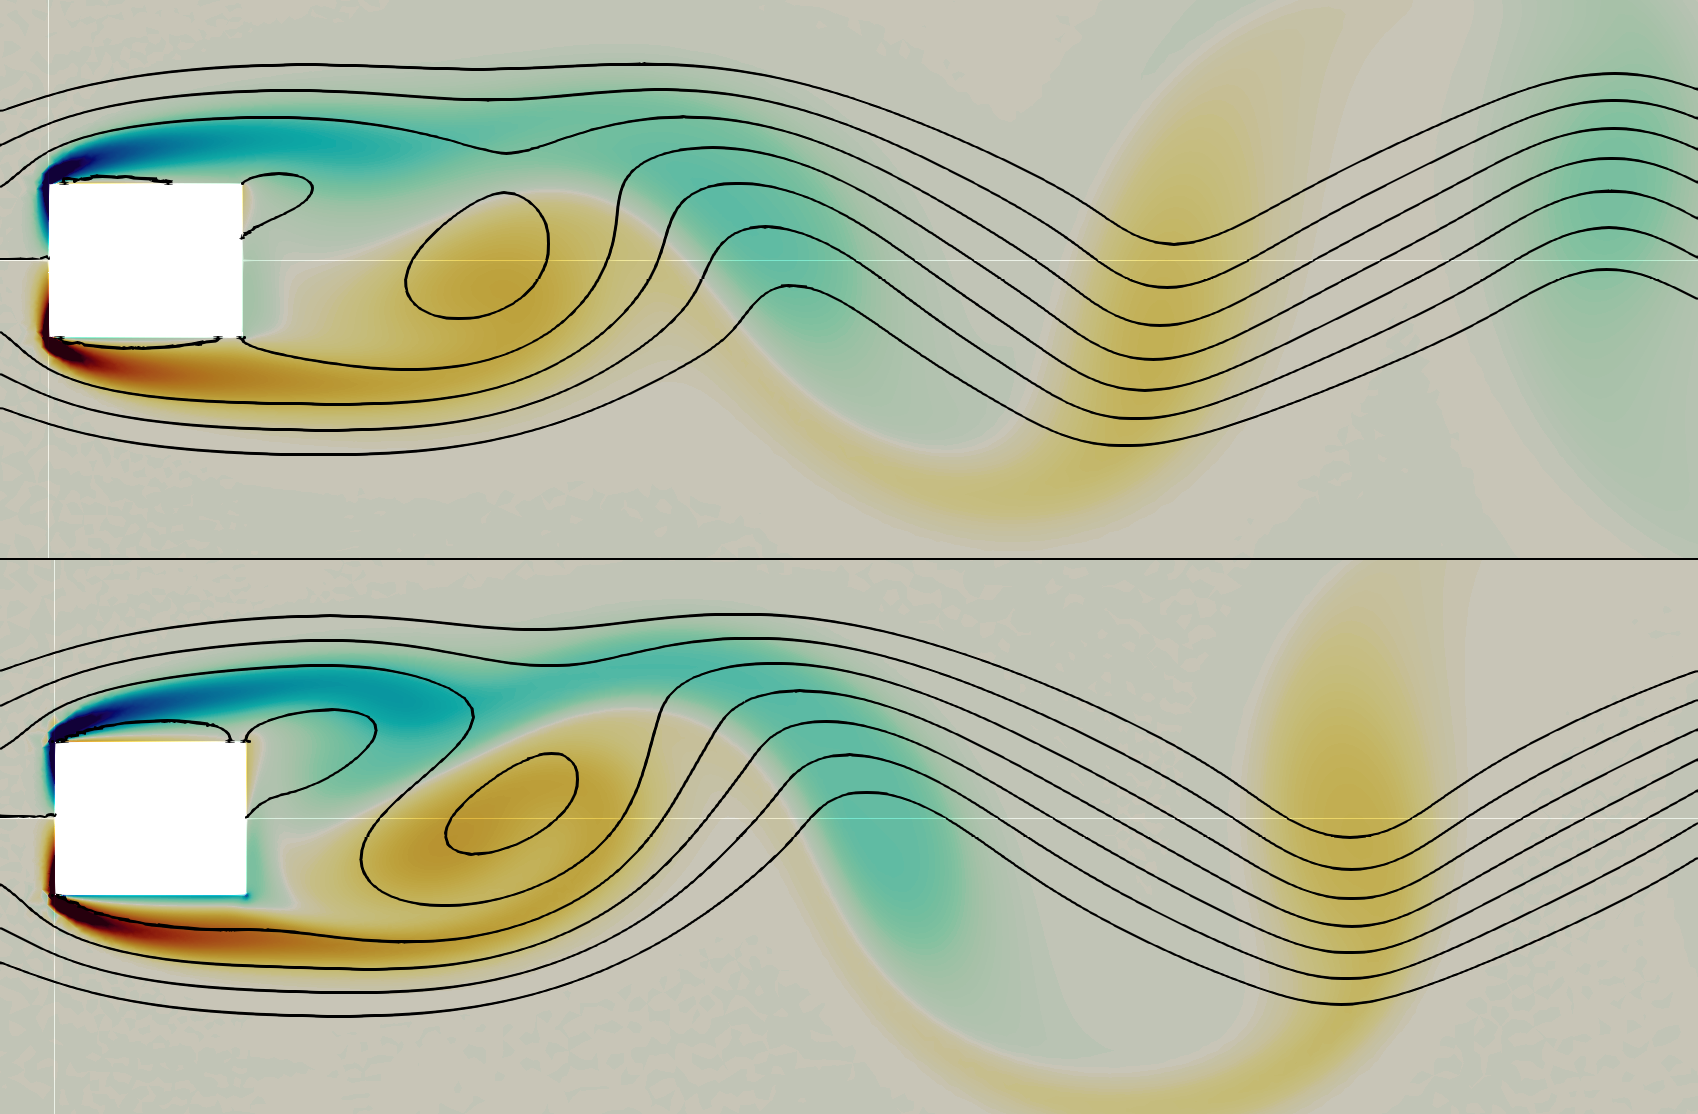
\includegraphics[width=0.49\textwidth]{./fig/AR1s/AR1p25_Re140_Re230_omegaz.png}
  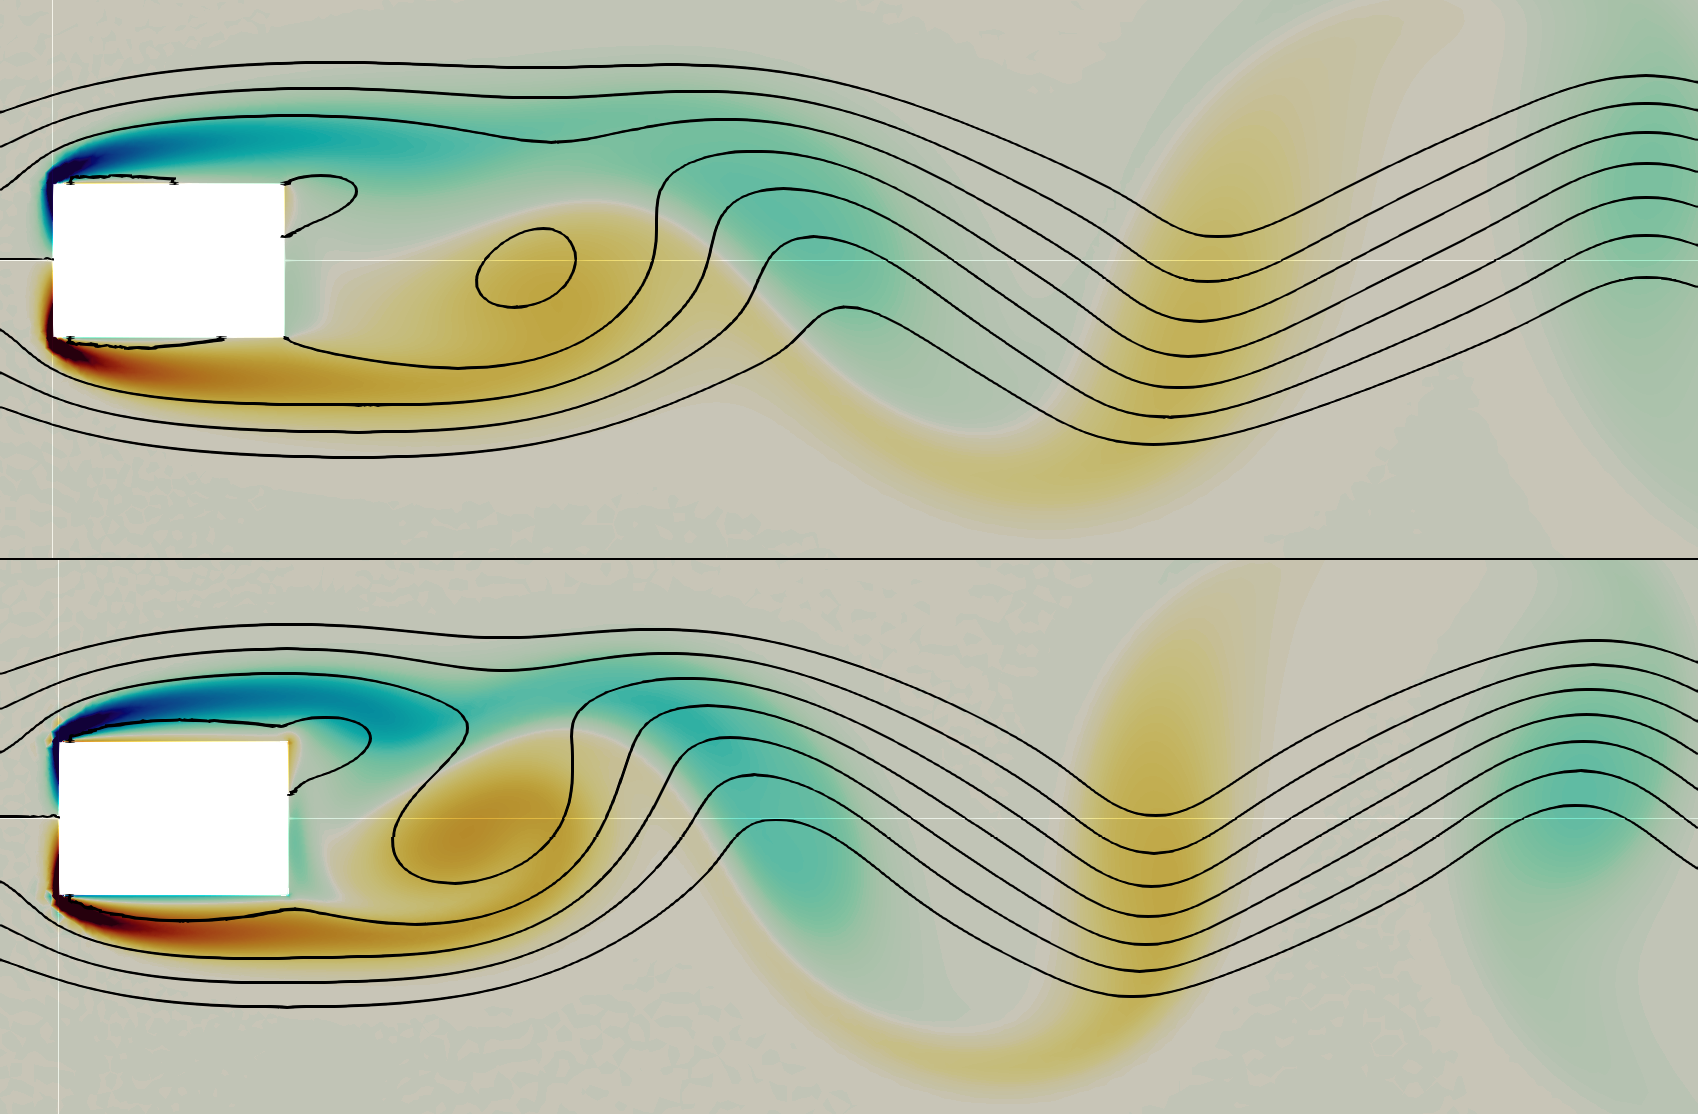
\includegraphics[width=0.49\textwidth]{./fig/AR1s/AR1p5_Re140_Re230_omegaz.png}
  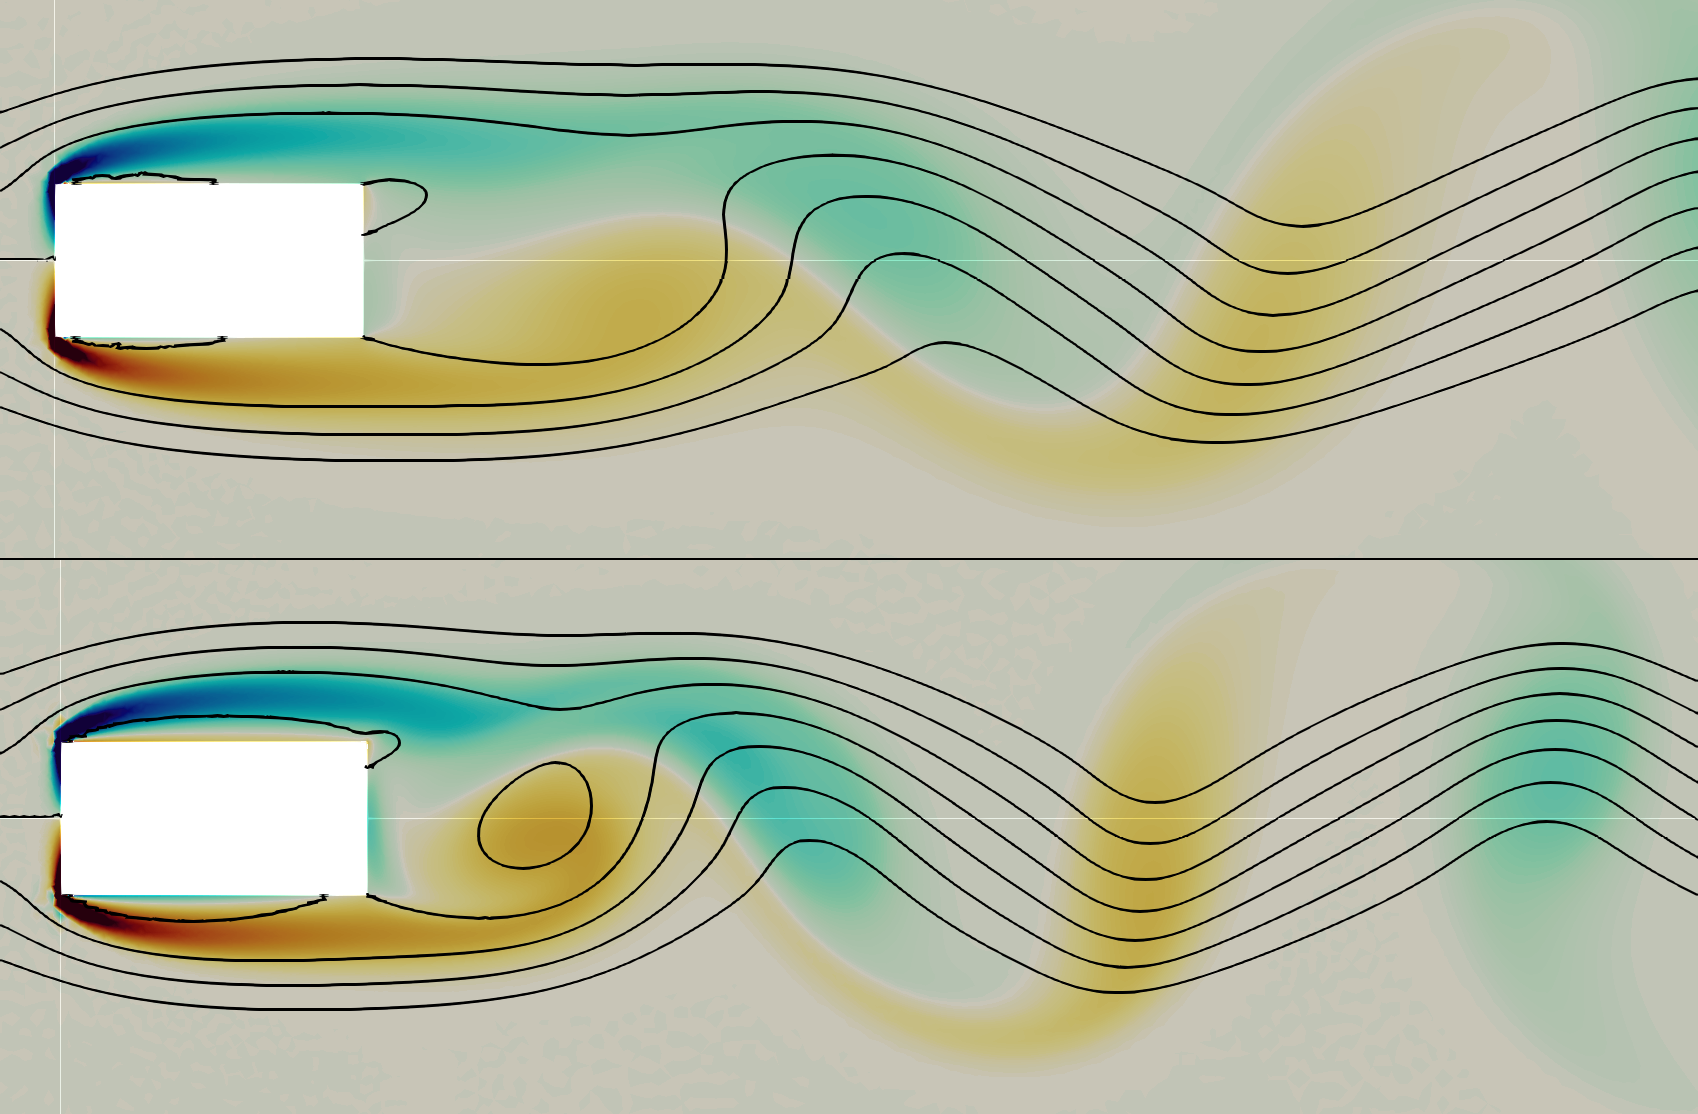
\includegraphics[width=0.49\textwidth]{./fig/AR1s/AR2_Re140_Re230_omegaz.png}
  \caption{Instantaneous visualisation of the flow for $Re=140$ (top) and $Re=230$ (bottom). Top left: $\AR=0.625$. Top right: $\AR=1.125$. Bottom left: $\AR=1.5$. Bottom right: $\AR=2$. The colour map denotes the spanwise vorticity in the $-10 \le \omega_z \le 10$ range. The black lines indicate the flow streamlines determined as isolines of $\psi$ spaces with $\pm 0.2$. XX IL CAMBIO DI ANDAMENTO DI $T$ SI VEDE QUANDO LA CORRENTE NON RIATTACCA PIU IN QUEL CASO COMINCIA DI NUOVO A CRESERE T. E' POSSIBILE VEDERLO, P.E. GUARDANDO IL CAMPO MEDIO XX}
  \label{fig:snap_Re140_Re230}
\end{figure}    


\begin{figure}
  \centering
  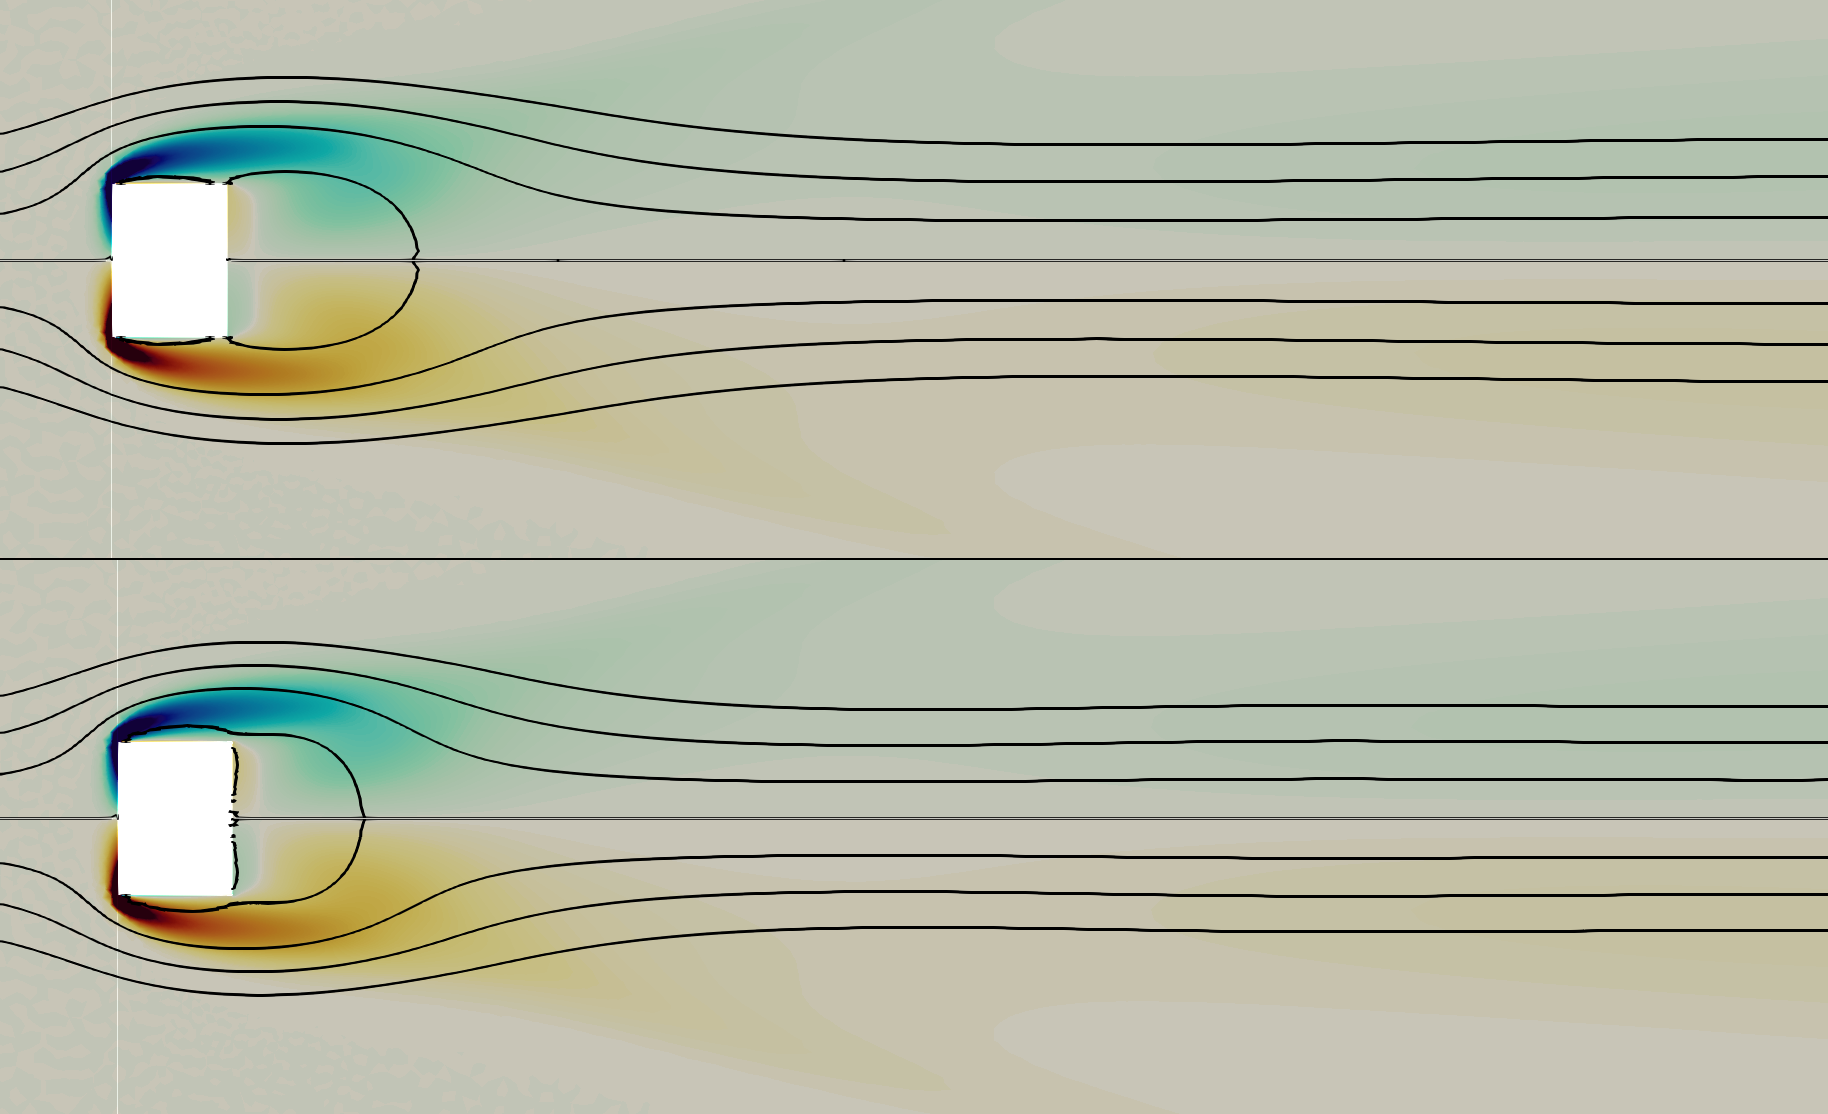
\includegraphics[width=0.49\textwidth]{./fig/AR1s/AR0p75_Re140_Re230_omegaz_Av.png}
  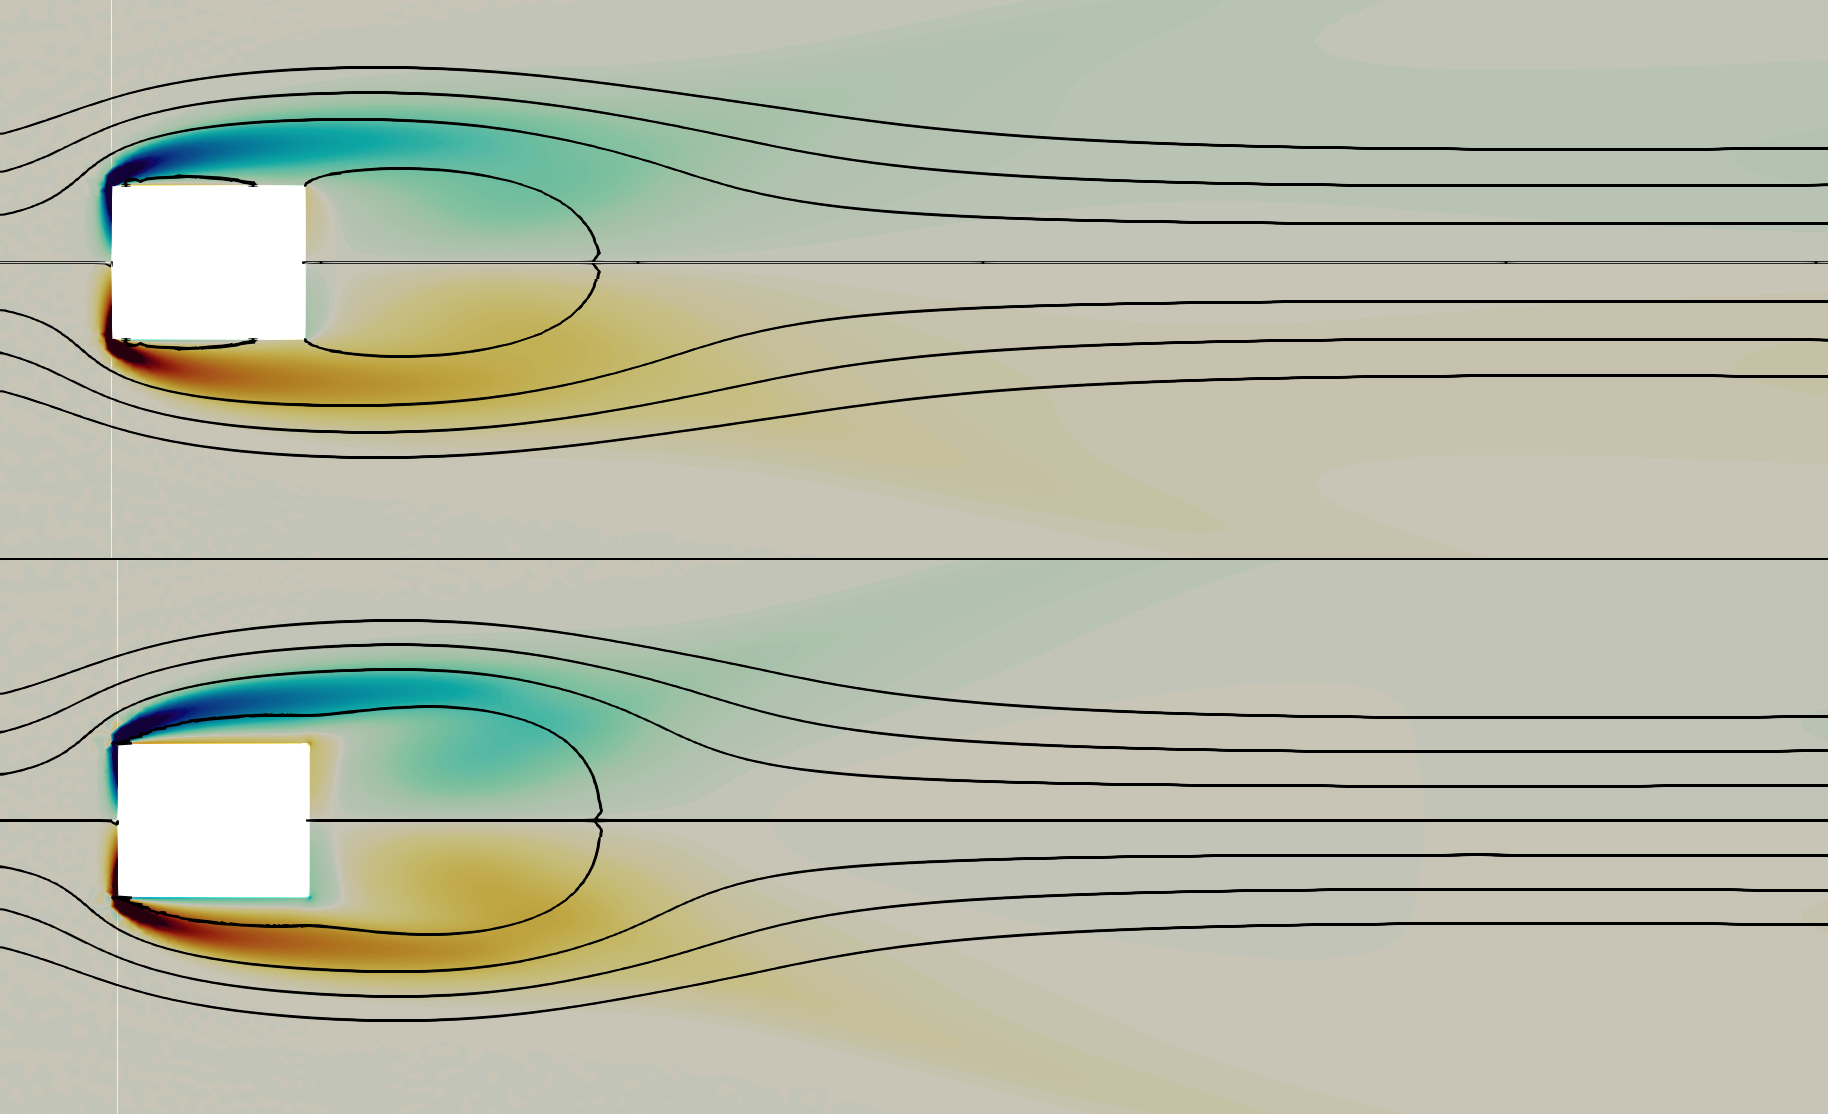
\includegraphics[width=0.49\textwidth]{./fig/AR1s/AR1p25_Re140_Re230_omegaz_Av.png}
  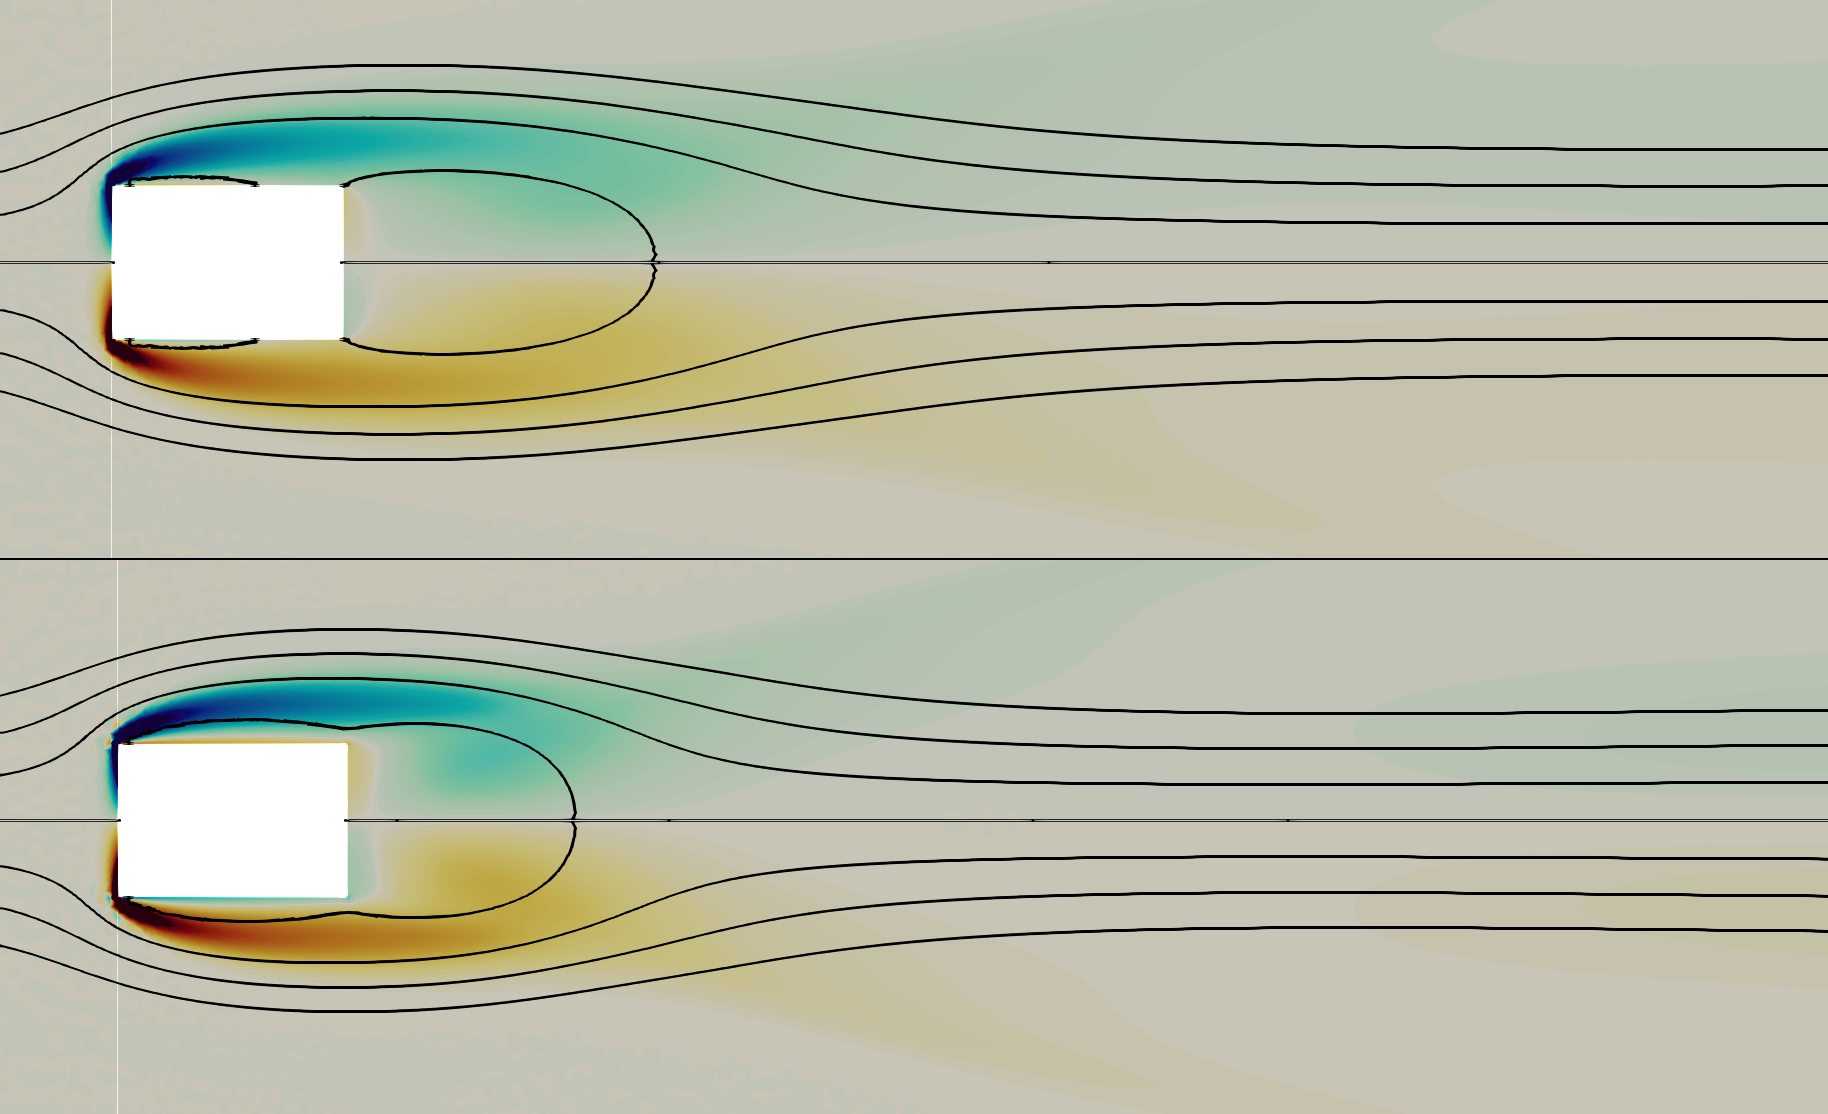
\includegraphics[width=0.49\textwidth]{./fig/AR1s/AR1p5_Re140_Re230_omegaz_Av.png}
  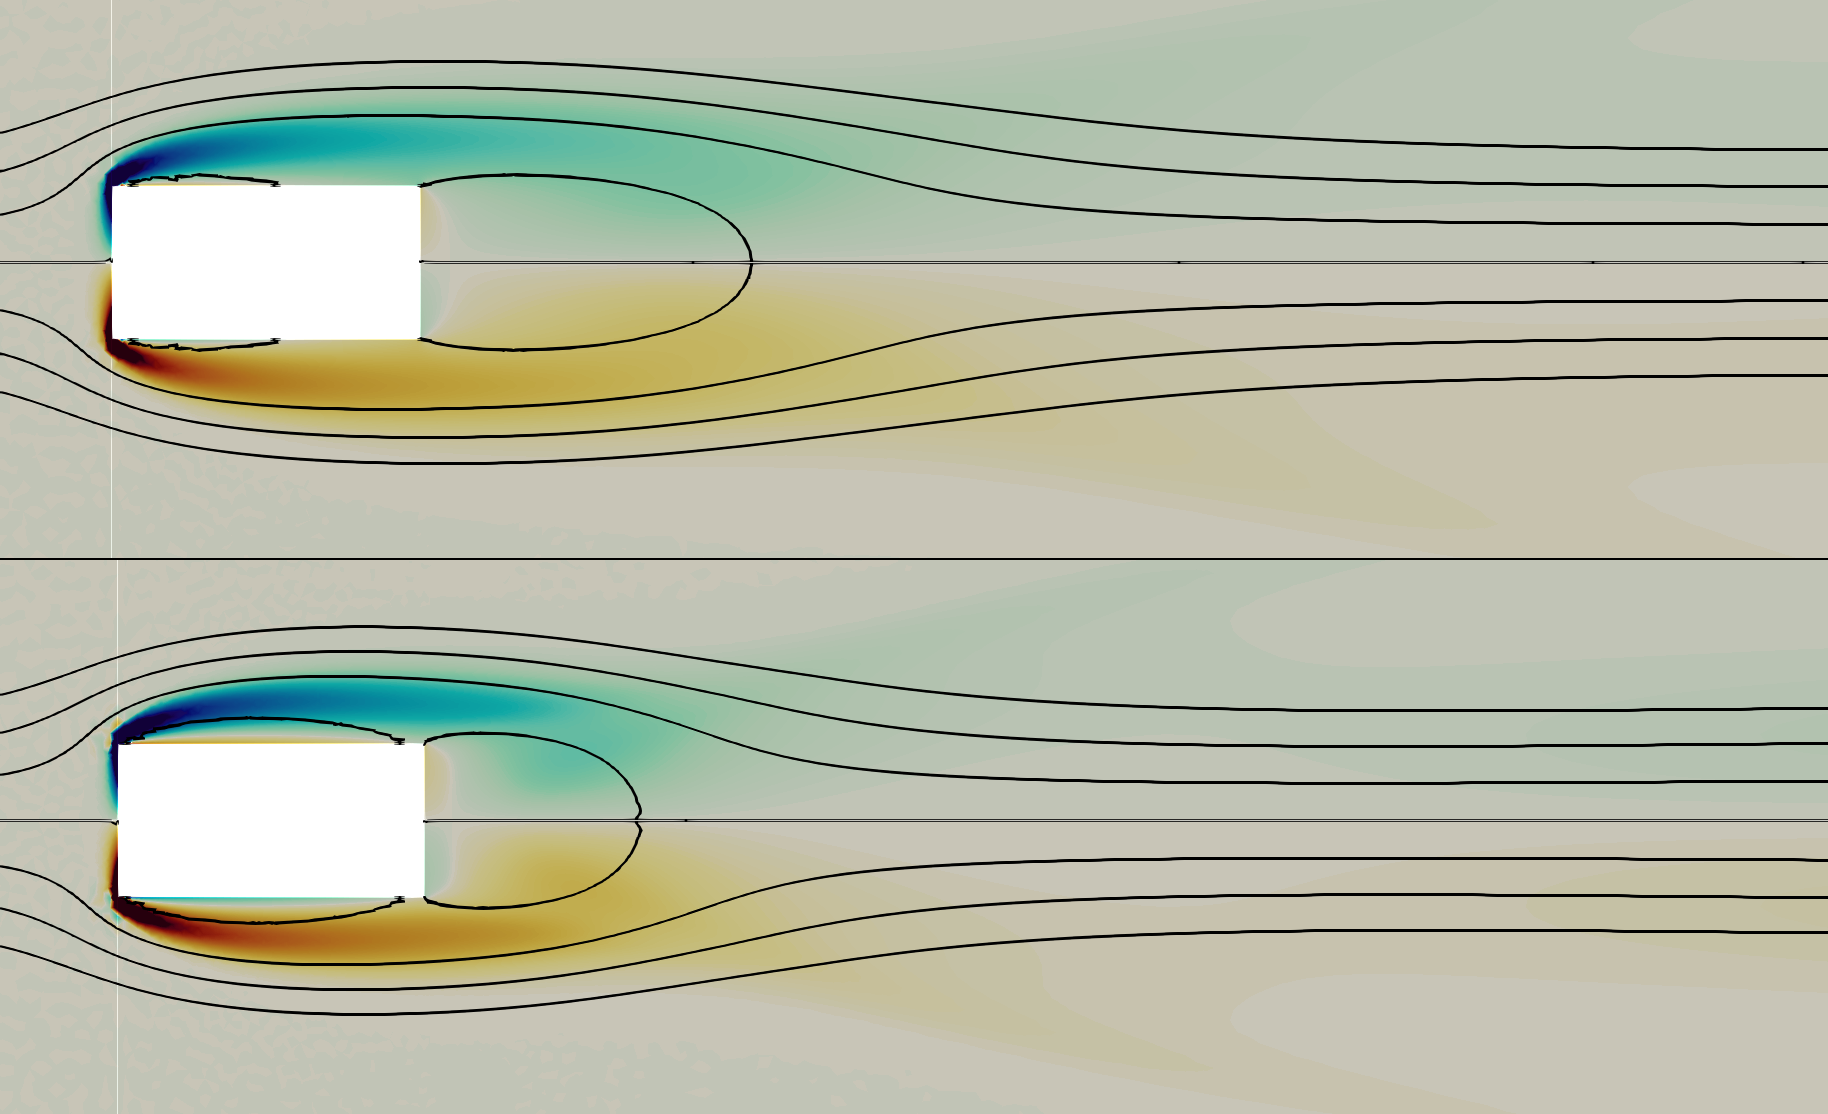
\includegraphics[width=0.49\textwidth]{./fig/AR1s/AR2_Re140_Re230_omegaz_Av.png}
  \caption{Visualisation of the mean flow for $Re=140$ (top) and $Re=230$ (bottom). Top left: $\AR=0.625$. Top right: $\AR=1.125$. Bottom left: $\AR=1.5$. Bottom right: $\AR=2$. The colour map denotes the spanwise vorticity in the $-10 \le \omega_z \le 10$ range. The black lines indicate the flow streamlines determined as isolines of $\psi$ spaces with $\pm 0.2$. XX IL CAMBIO DI ANDAMENTO DI $T$ SI VEDE QUANDO LA CORRENTE NON RIATTACCA PIU IN QUEL CASO COMINCIA DI NUOVO A CRESERE T. E' POSSIBILE VEDERLO, P.E. GUARDANDO IL CAMPO MEDIO XX}
  \label{fig:Av_Re140_Re230}
\end{figure} 

The varying trends in the shedding period $T$ with Reynolds number across aspect ratios reflect changes in the base-flow topology and in the underlying vortex shedding mechanisms. These are illustrated in figures~\ref{fig:snap_Re140_Re230} and \ref{fig:Av_Re140_Re230}, which show instantaneous and time-averaged flow fields for $Re=140$ and $Re=230$, across different $\AR$.
%
For shorter bodies ($\AR \lessapprox 1$), the flow separates at the LE corners and only rarely reattaches along the lateral sides, regardless of $Re$. In this regime, vortex shedding is primarily governed by the dynamics of the LE shear layer, which actively participates in the formation of the wake vortex. As shown in figure \ref{fig:snap_Re140_Re230}, the LE shear layer delineates the boundary of the vortex as it is shed downstream.
%
In contrast, for longer bodies ($\AR \gtrapprox 1.5$), the LE shear layer reattaches along the lateral sides across all considered $Re$, and the vortex shedding is predominantly driven by the TE shear layers. For the intermediate case ($1 \lessapprox \AR \lessapprox 1.5$), the base-flow topology varies with Reynolds number: at lower $Re$, the flow resembles that of longer bodies, with intermittent reattachment of the LE shear layer and shedding governed by the TE. At higher $Re$, however, the flow shifts toward the low-$\AR$ topology, with the LE shear layer again playing the dominant role in vortex formation.
%
This transition is reflected in the behaviour of the shedding period $T$ in figure~\ref{fig:T_Re_small}(b). When vortex shedding is LE-driven, $T$ increases with $Re$, likely due to interactions between the LE shear layer and the TE corners. Conversely, when the LE shear layer reattaches and shedding is driven by the TE, $T$ decreases with increasing $Re$. This shift in topology is consistent with the increasing separation angle at the LE corners as $Re$ rises. Furthermore, the critical Reynolds number at which this topological transition occurs increases with $\AR$, as evidenced by the turning points in the $T-Re$ curves in figure~\ref{fig:T_Re_small}(b).

\begin{table}
  \begin{center}
  \begin{tabular}{ccccccccc}
    $\AR$  & & $Re$  & & $\Re(\sigma)$ & & $St_{lin}$ & & $St_{nl}$ \\
    $0.75$ & & $140$ & & $-0.0065$  & & $0.1612$   & & $0.1616$  \\
    $0.75$ & & $230$ & & $-0.0159$  & & $0.1660$   & & $0.1653$  \\
    $1.25$ & & $140$ & & $-0.0134$  & & $0.1517$   & & $0.1519$  \\
    $1.25$ & & $230$ & & $-0.0393$  & & $0.1360$   & & $0.1350$  \\
    $1.50$ & & $140$ & & $-0.0126$  & & $0.1502$   & & $0.1512$  \\
    $1.50$ & & $230$ & & $-0.0394$  & & $0.1647$   & & $0.1625$  \\
    $2.00$ & & $140$ & & $-0.0037$  & & $0.1465$   & & $0.1483$  \\
    $2.00$ & & $230$ & & $-0.0124$  & & $0.1744$   & & $0.1695$  \\
  \end{tabular} 
  \caption{XX}
  \label{tab:eigs}
  \end{center}  
\end{table}
%
\begin{figure}
  \centering
  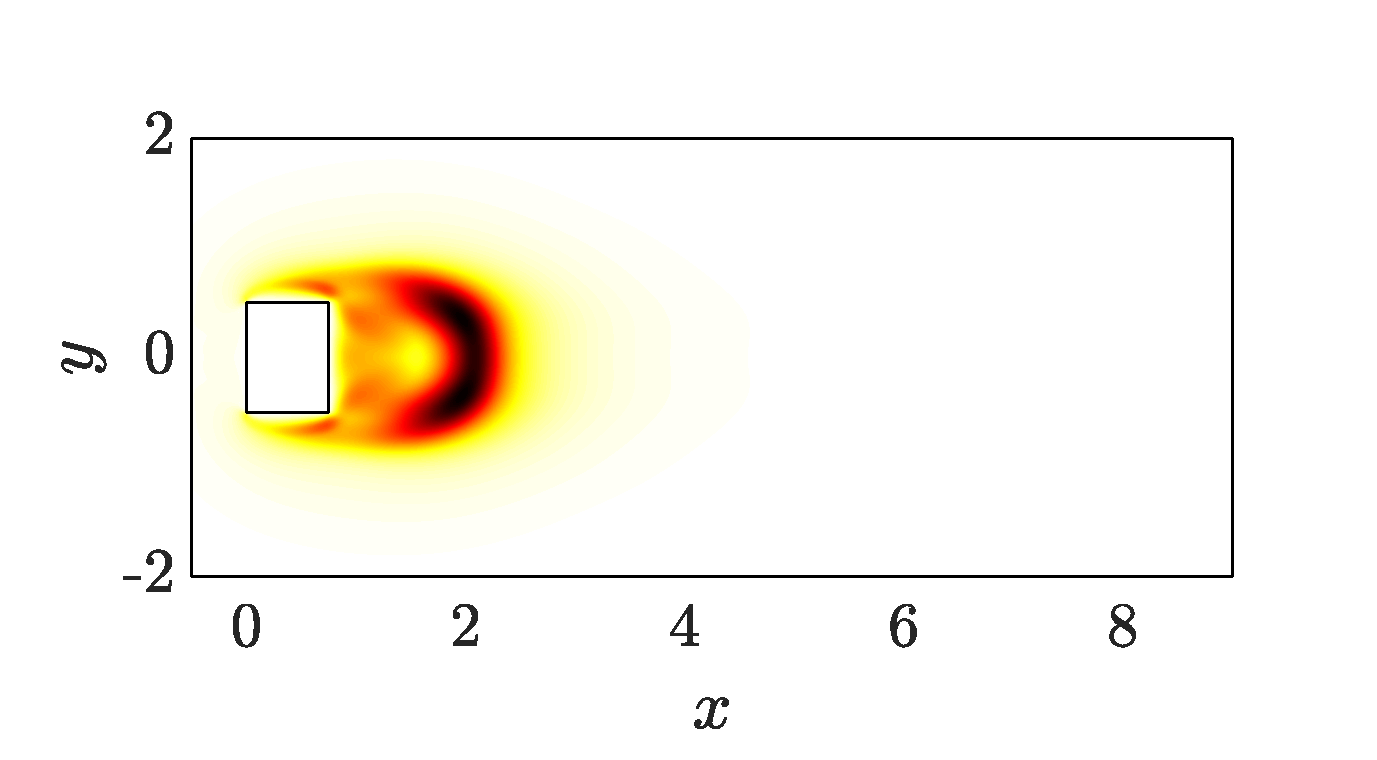
\includegraphics[width=0.49\textwidth]{./fig/AR1s/sens_AR0p75_Re140.eps}
  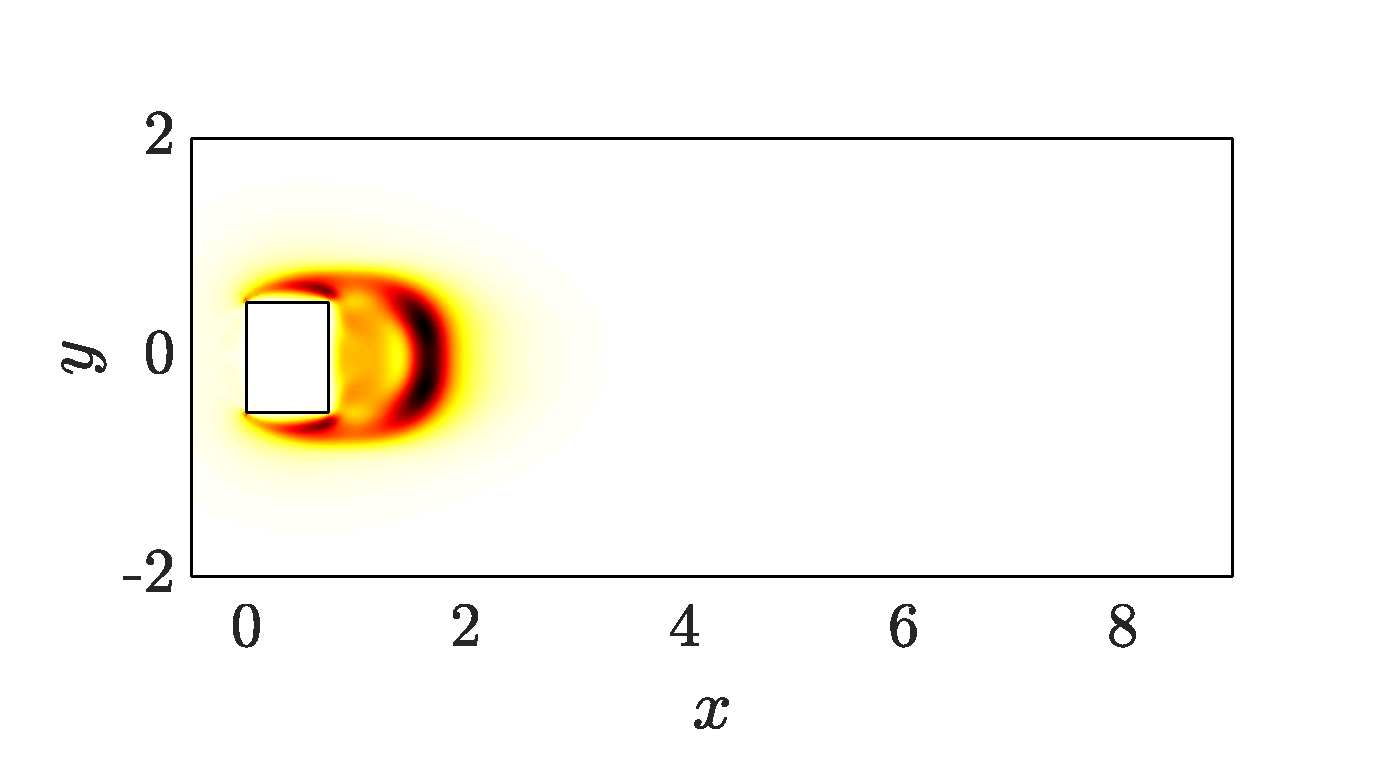
\includegraphics[width=0.49\textwidth]{./fig/AR1s/sens_AR0p75_Re230.eps} 
  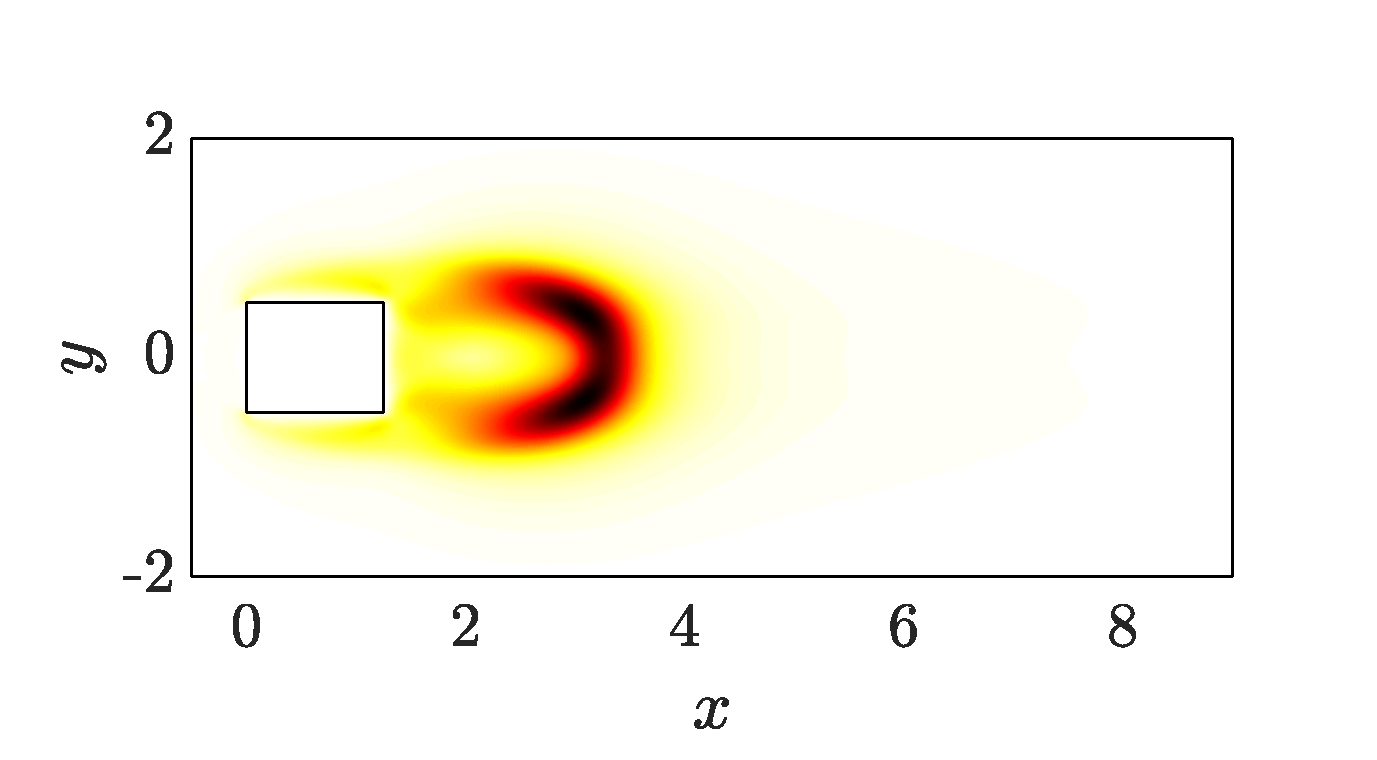
\includegraphics[width=0.49\textwidth]{./fig/AR1s/sens_AR1p25_Re140.eps}
  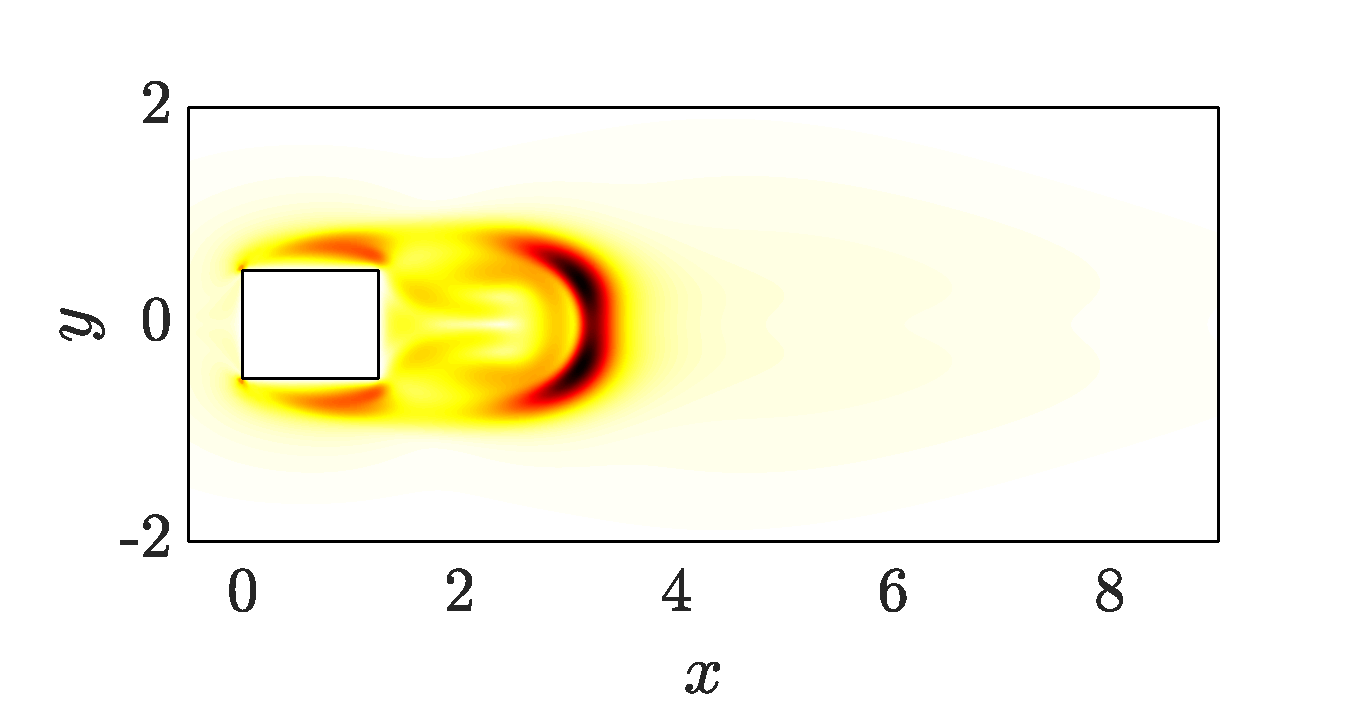
\includegraphics[width=0.49\textwidth]{./fig/AR1s/sens_AR1p25_Re230.eps}   
%  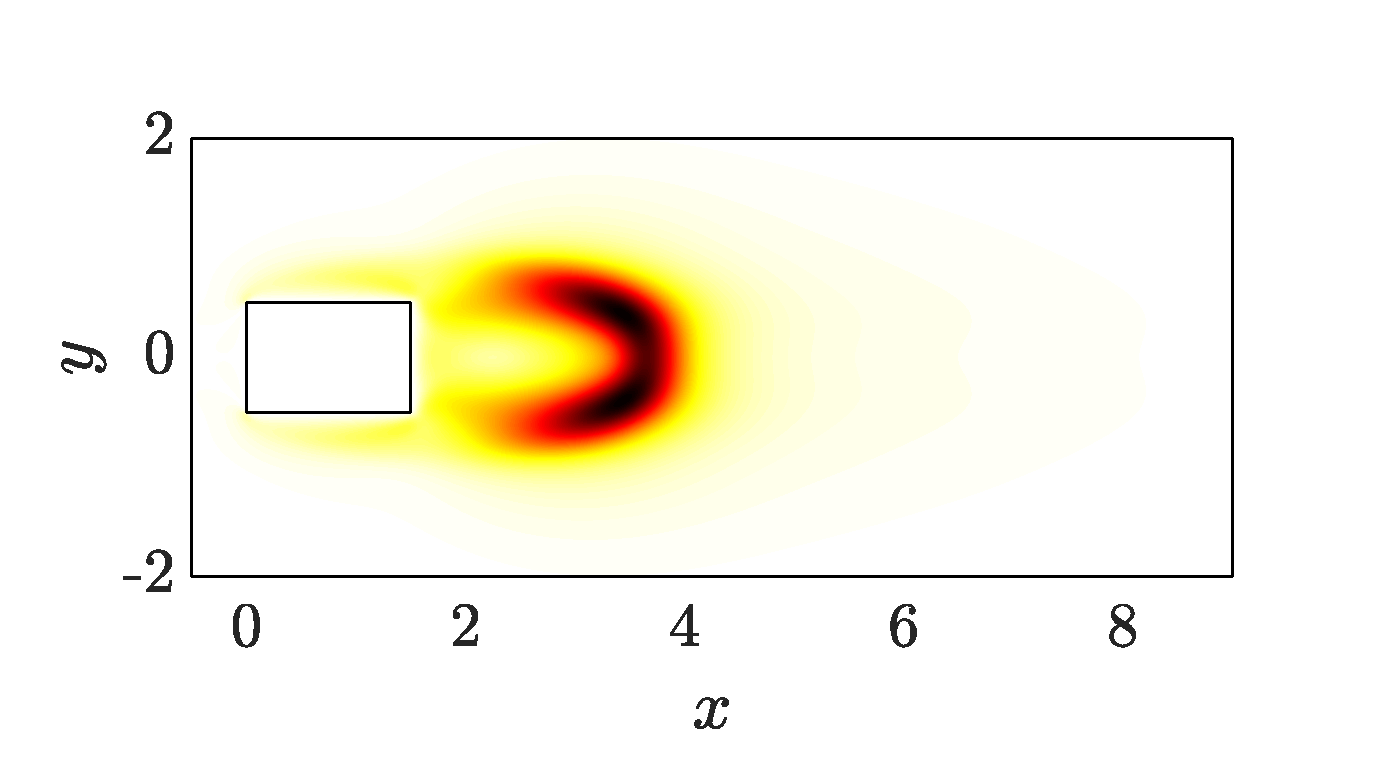
\includegraphics[width=0.49\textwidth]{./fig/AR1s/sens_AR1p5_Re140.eps}
%  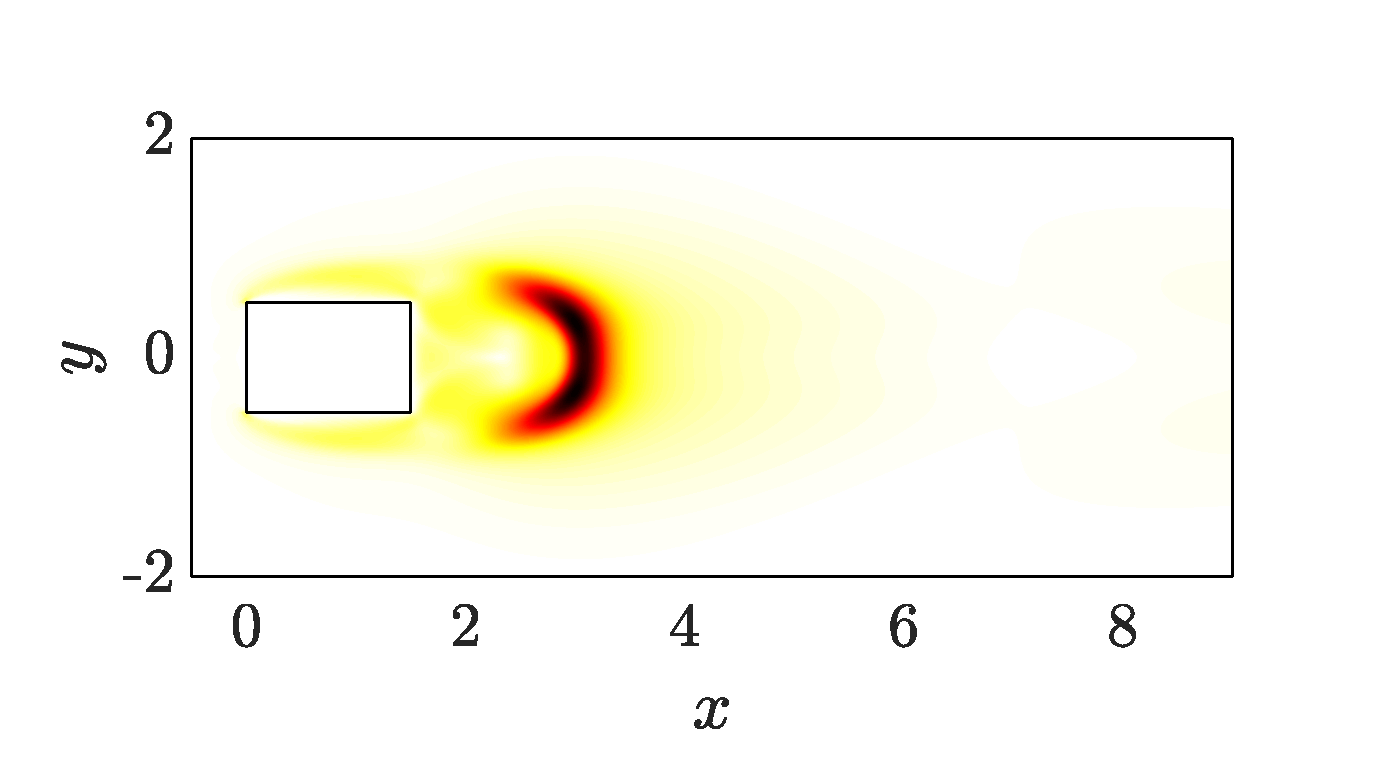
\includegraphics[width=0.49\textwidth]{./fig/AR1s/sens_AR1p5_Re230.eps} 
  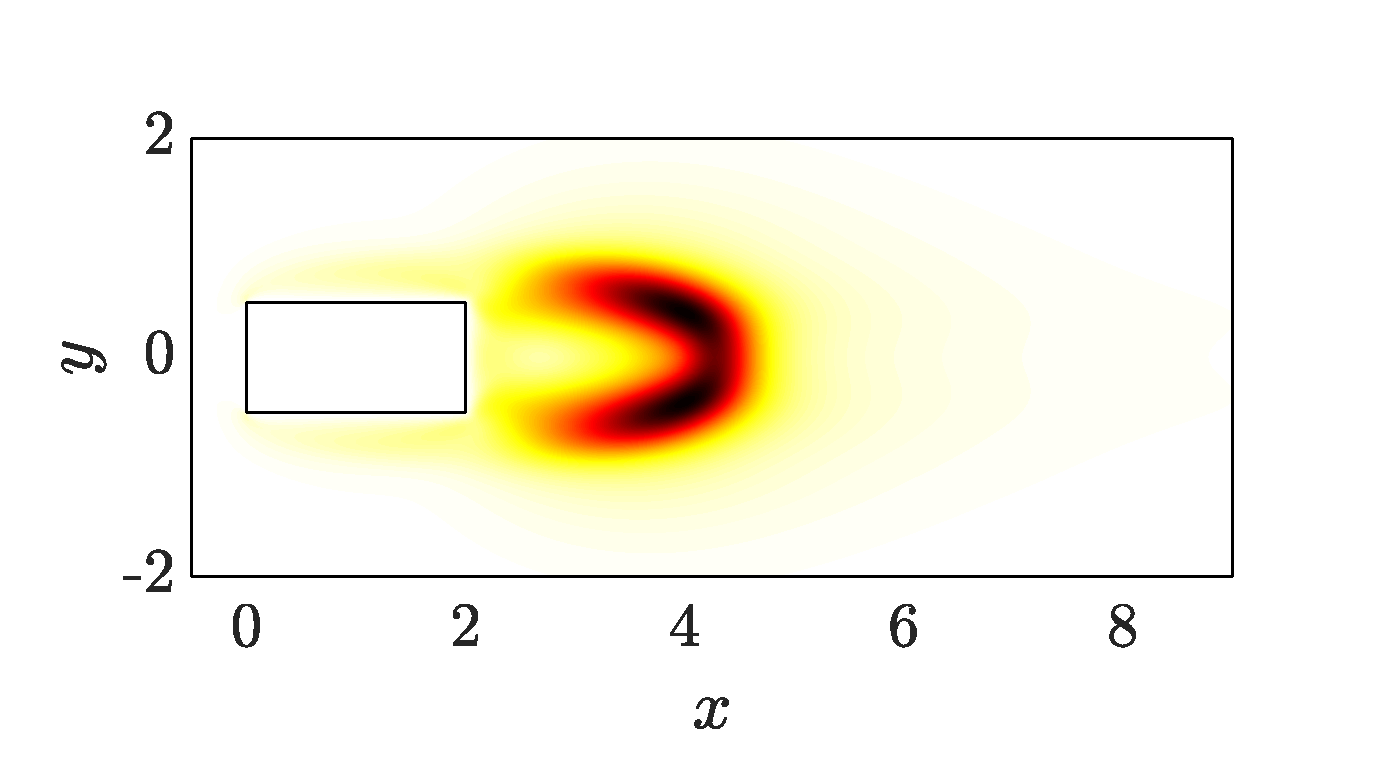
\includegraphics[width=0.49\textwidth]{./fig/AR1s/sens_AR2_Re140.eps}
  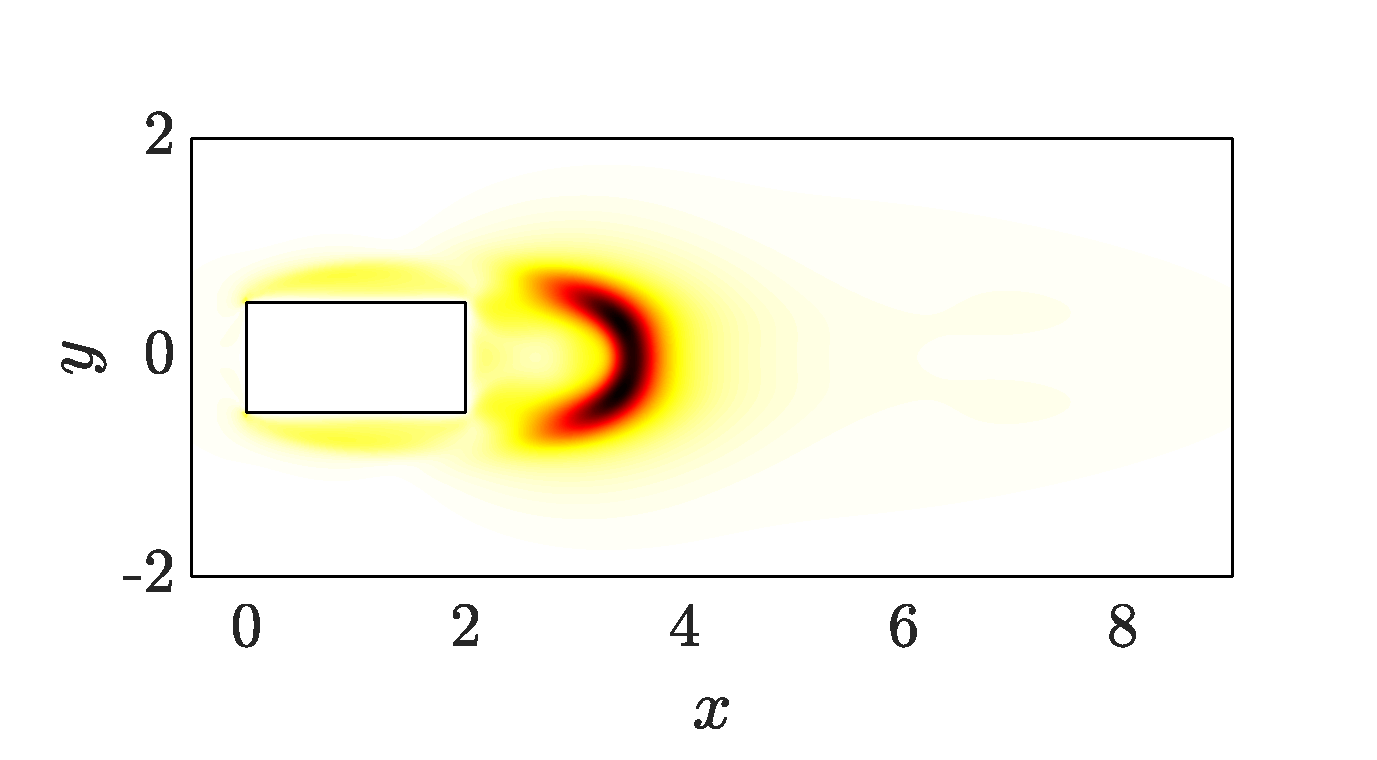
\includegraphics[width=0.49\textwidth]{./fig/AR1s/sens_AR2_Re230.eps}  
  \caption{XX SI VEDE LA DIFFERENZA. PER $\AR$ PICCOLI LO SHEDDING È DOMINATO DALLO SHEAR LAYER CHE SEPARA DAL LE. PER $\AR$ INTERMEDI, LO SHEDDING A RE BASSI È DOMINATO DAL TE SHEAR LAYER, MENTRE A RE ALTI ANCHE DAL LE SHEAR LAYER. PER $\AR$ ALTI, LO SHEDDING È DOMINATO DAL TE SHEAR LAYER PER TUTTI I RE. XX}
  \label{fig:sens-short}
\end{figure}    
%
To further investigate how flow dyanamics varies with aspect ratio $\AR$ and Reynolds number $Re$, we perform a global stability analysis of the mean flow, averaged over one shedding period. We focus on the leading eigenmode, which captures the dominant unsteady features of the flow. Similar approaches have been applied to the circular cylinder \citep{pier-2002, barkley-2006} and to elongated rectangular cylinders \citep{chiarini-quadrio-auteri-2022}.
%
The frequency of the leading eigenmode provides a good estimate of the Strouhal number observed in the nonlinear simulations across all cases, see table~\ref{tab:eigs}. Unlike the marginally stable mean flow observed for the circular cylinder \citep{barkley-2006}, our analysis yields slightly negative growth rates, suggesting a weakly damped but still dynamically relevant mean flow instability.

Figure~\ref{fig:sens-short} shows the structural sensitivity of the leading eigenmode. This quantity, introduced by \cite{giannetti-luchini-2007}, provides an upper bound on the variation of the eigenvalue resulting from a localised perturbation of the linearised Navier--Stokes operator. It corresponds to a ``force-velocity'' coupling: the feedback from a localised velocity sensor to a colocated force actuator. As such, structural sensitivity serves as an indicator of the eigenvalue's sensitivity to flow modifications and identifies the so-called wavemaker region \citep{monkewitz-etal-1993}---the core region responsible for the instability.
%
The structural sensitivity field reveals that the wavemaker is generally concentrated near the body, where the overlap of the direct and adjoint modes is largest. For longer bodies and lower $Re$, non-zero sensitivity is confined to the wake downstream of the TE, especially along the streamline bounding the mean recirculation zone. This confirms that, in these cases, the instability is driven primarily by the TE shear layers.
%
In contrast, for shorter bodies and/or higher $Re$, significant sensitivity also appears along the LE shear layers over the lateral sides. This indicates that the wavemaker extends upstream, confirming that the LE shear layers actively contribute to the vortex shedding mechanism. Overall, these results are consistent with the earlier discussion on the transition in flow topology and the corresponding changes in the shedding dynamics.


\iffalse


\begin{figure}
  \centering
  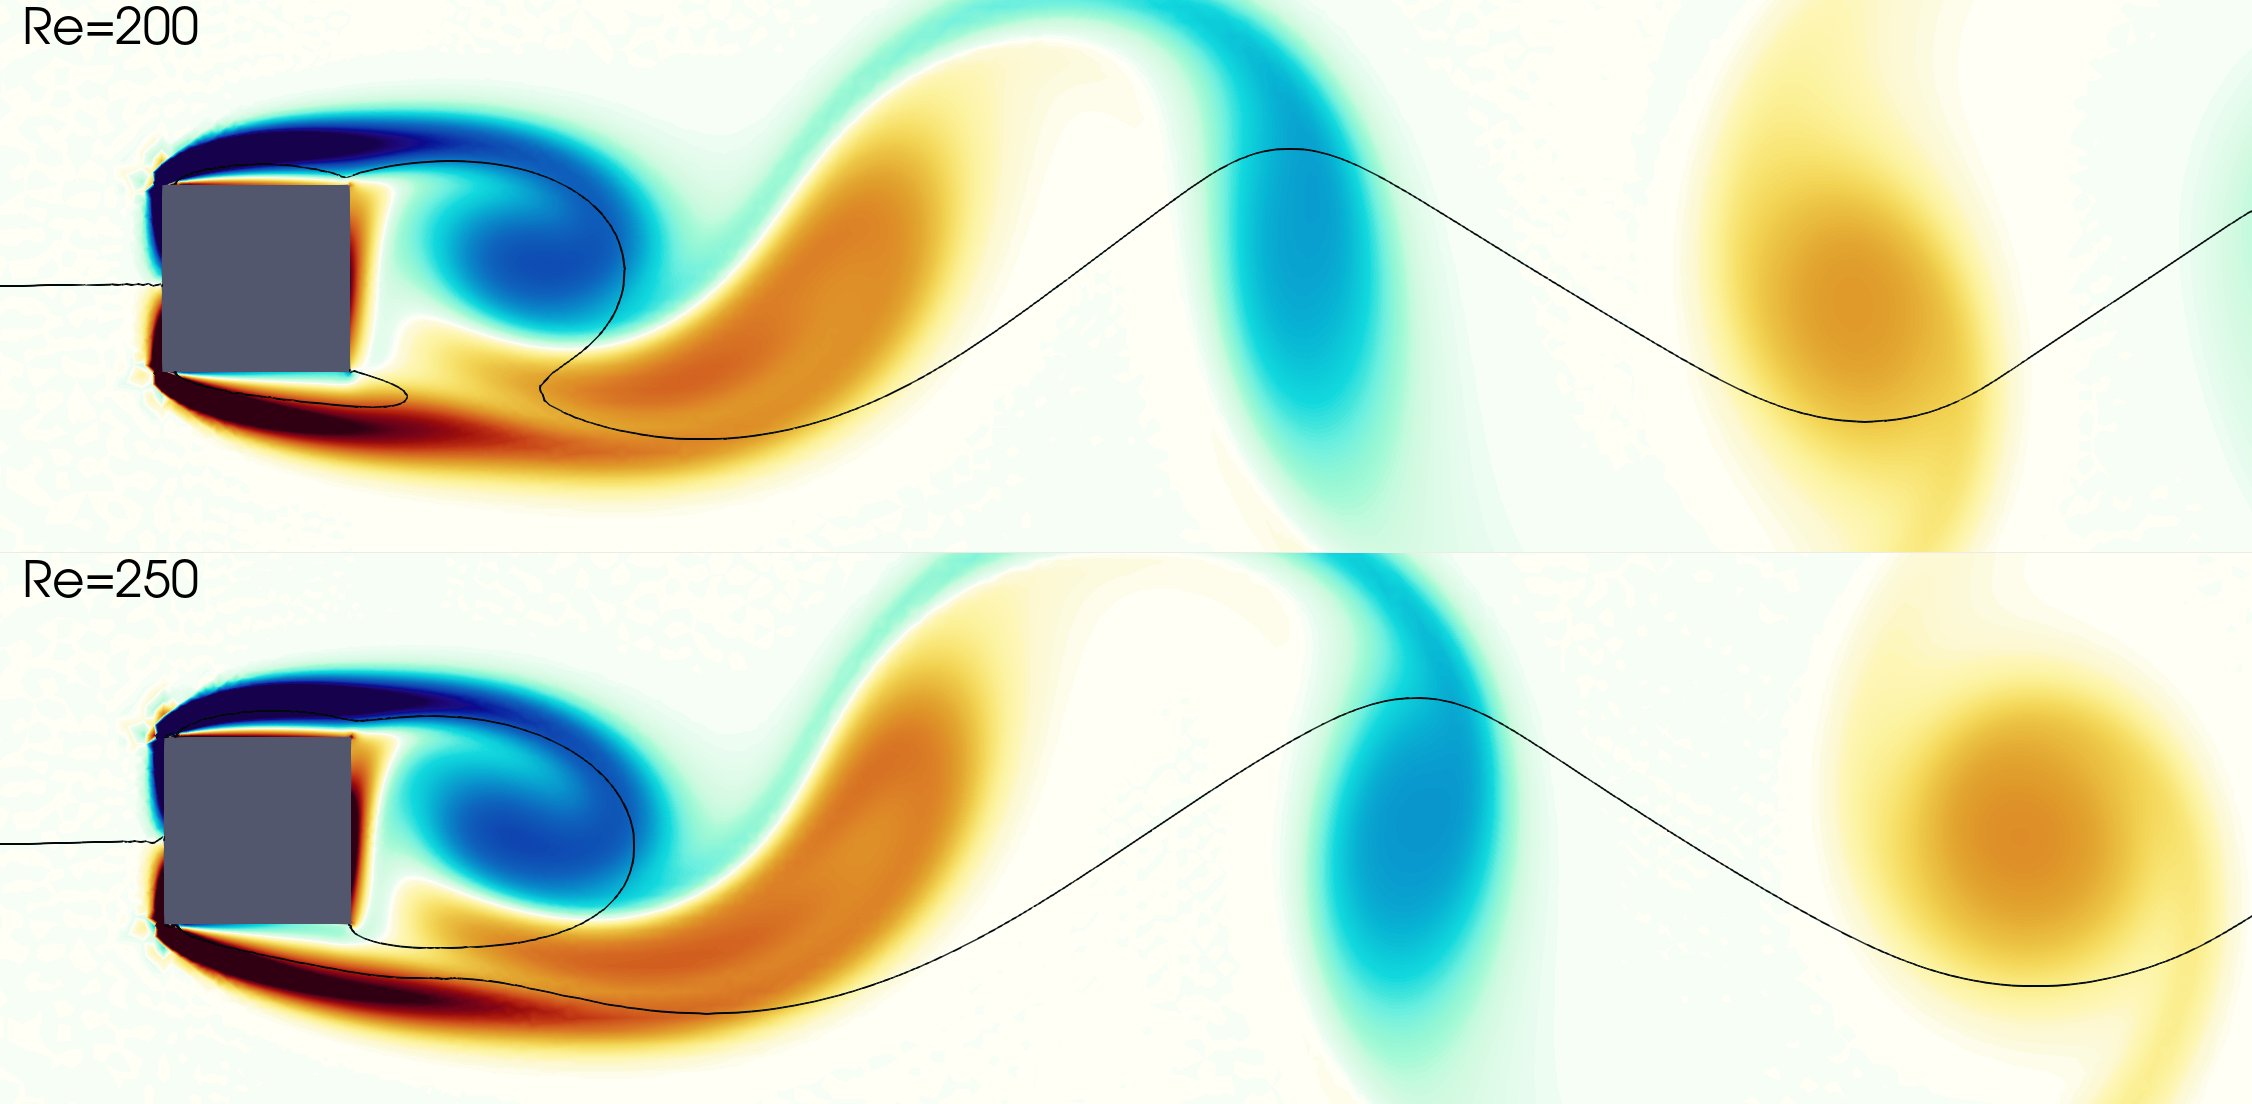
\includegraphics[width=0.49\textwidth]{./fig/AR1/snap/snap.0030.png}
  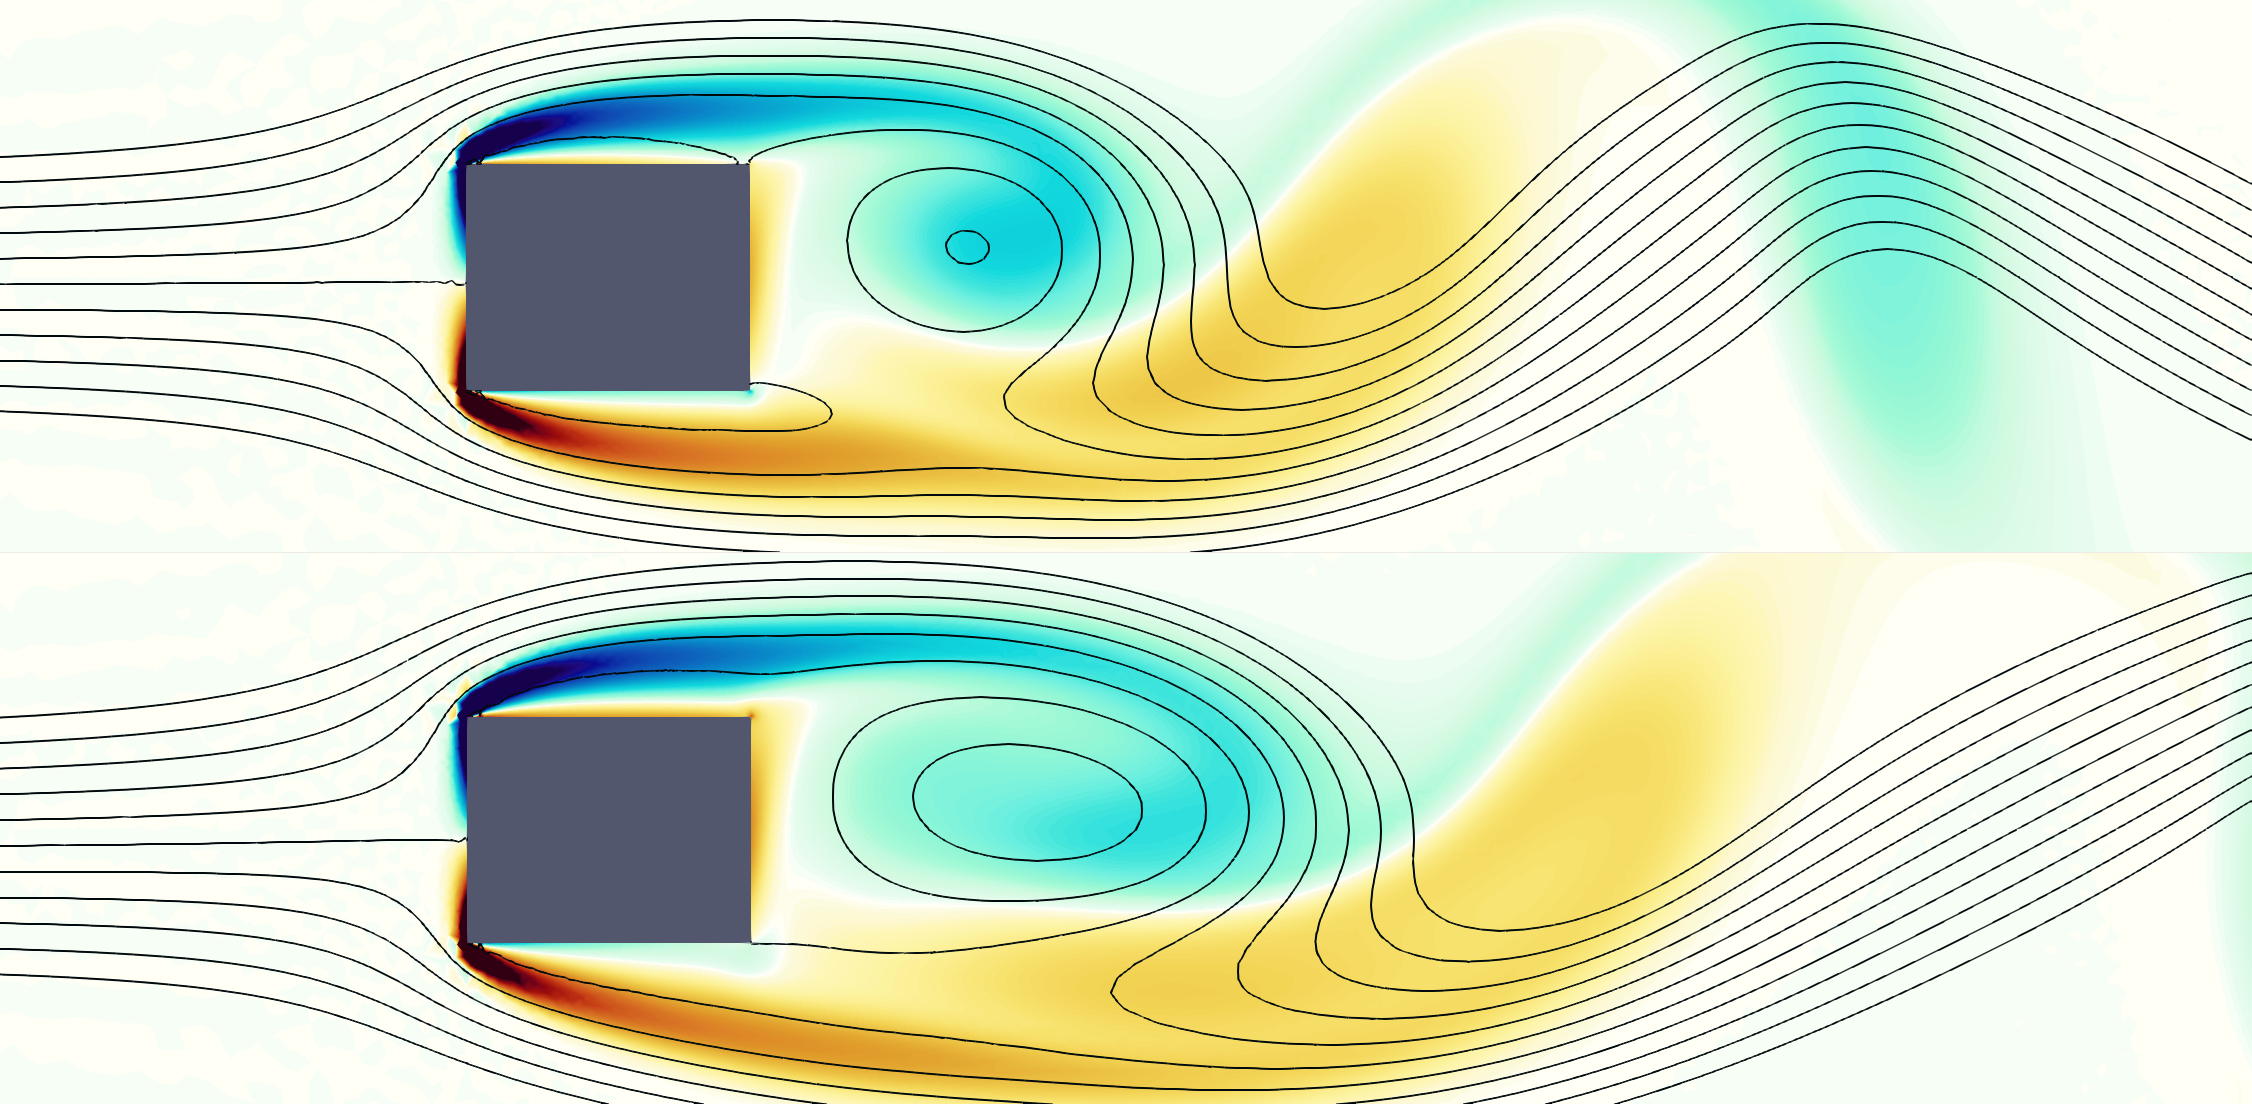
\includegraphics[width=0.49\textwidth]{./fig/AR1p25/snap/snap.0030.png}
  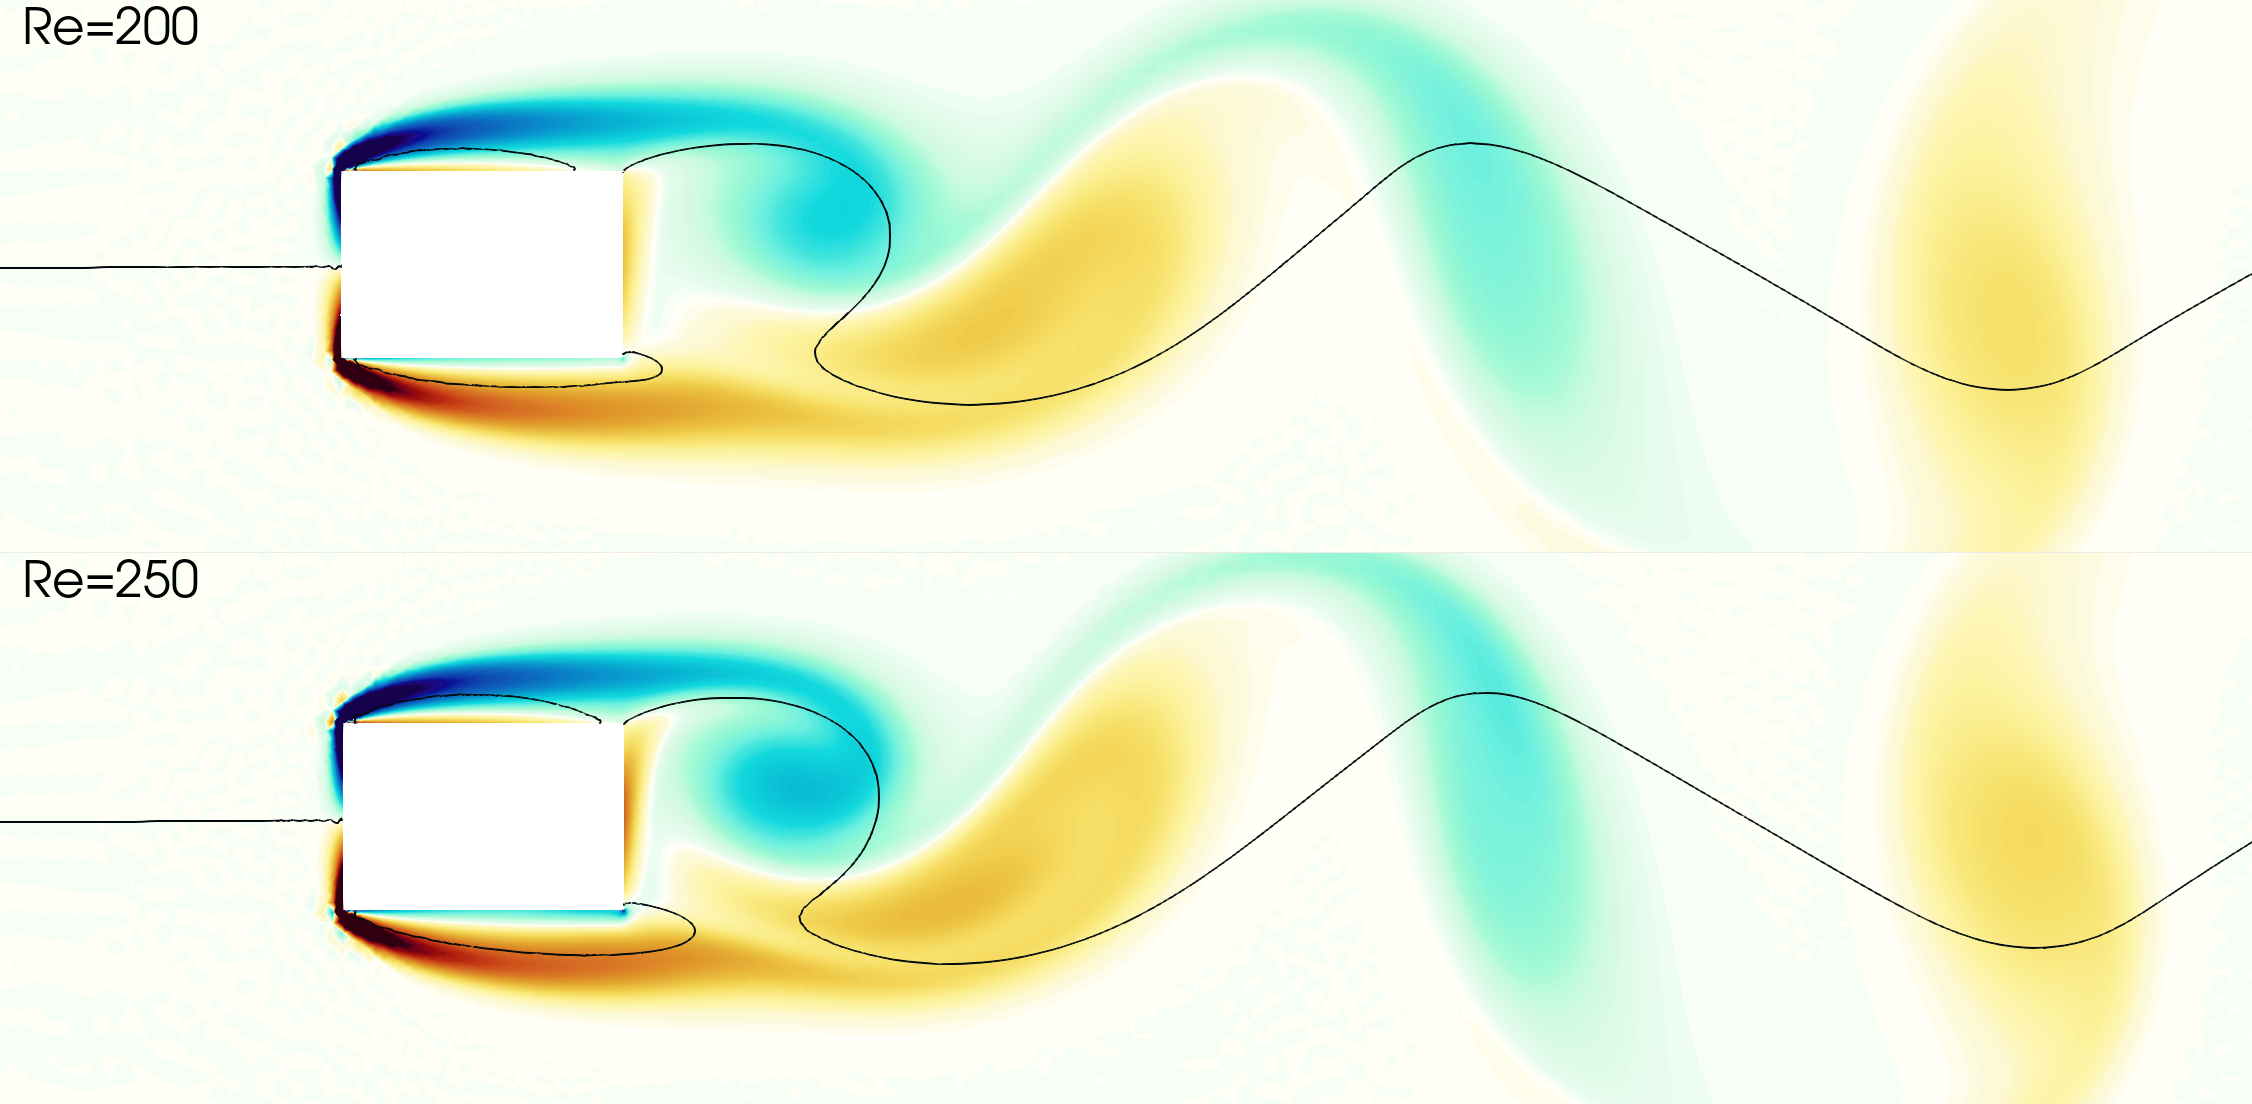
\includegraphics[width=0.49\textwidth]{./fig/AR1p5/snap/snap.0030.png}
  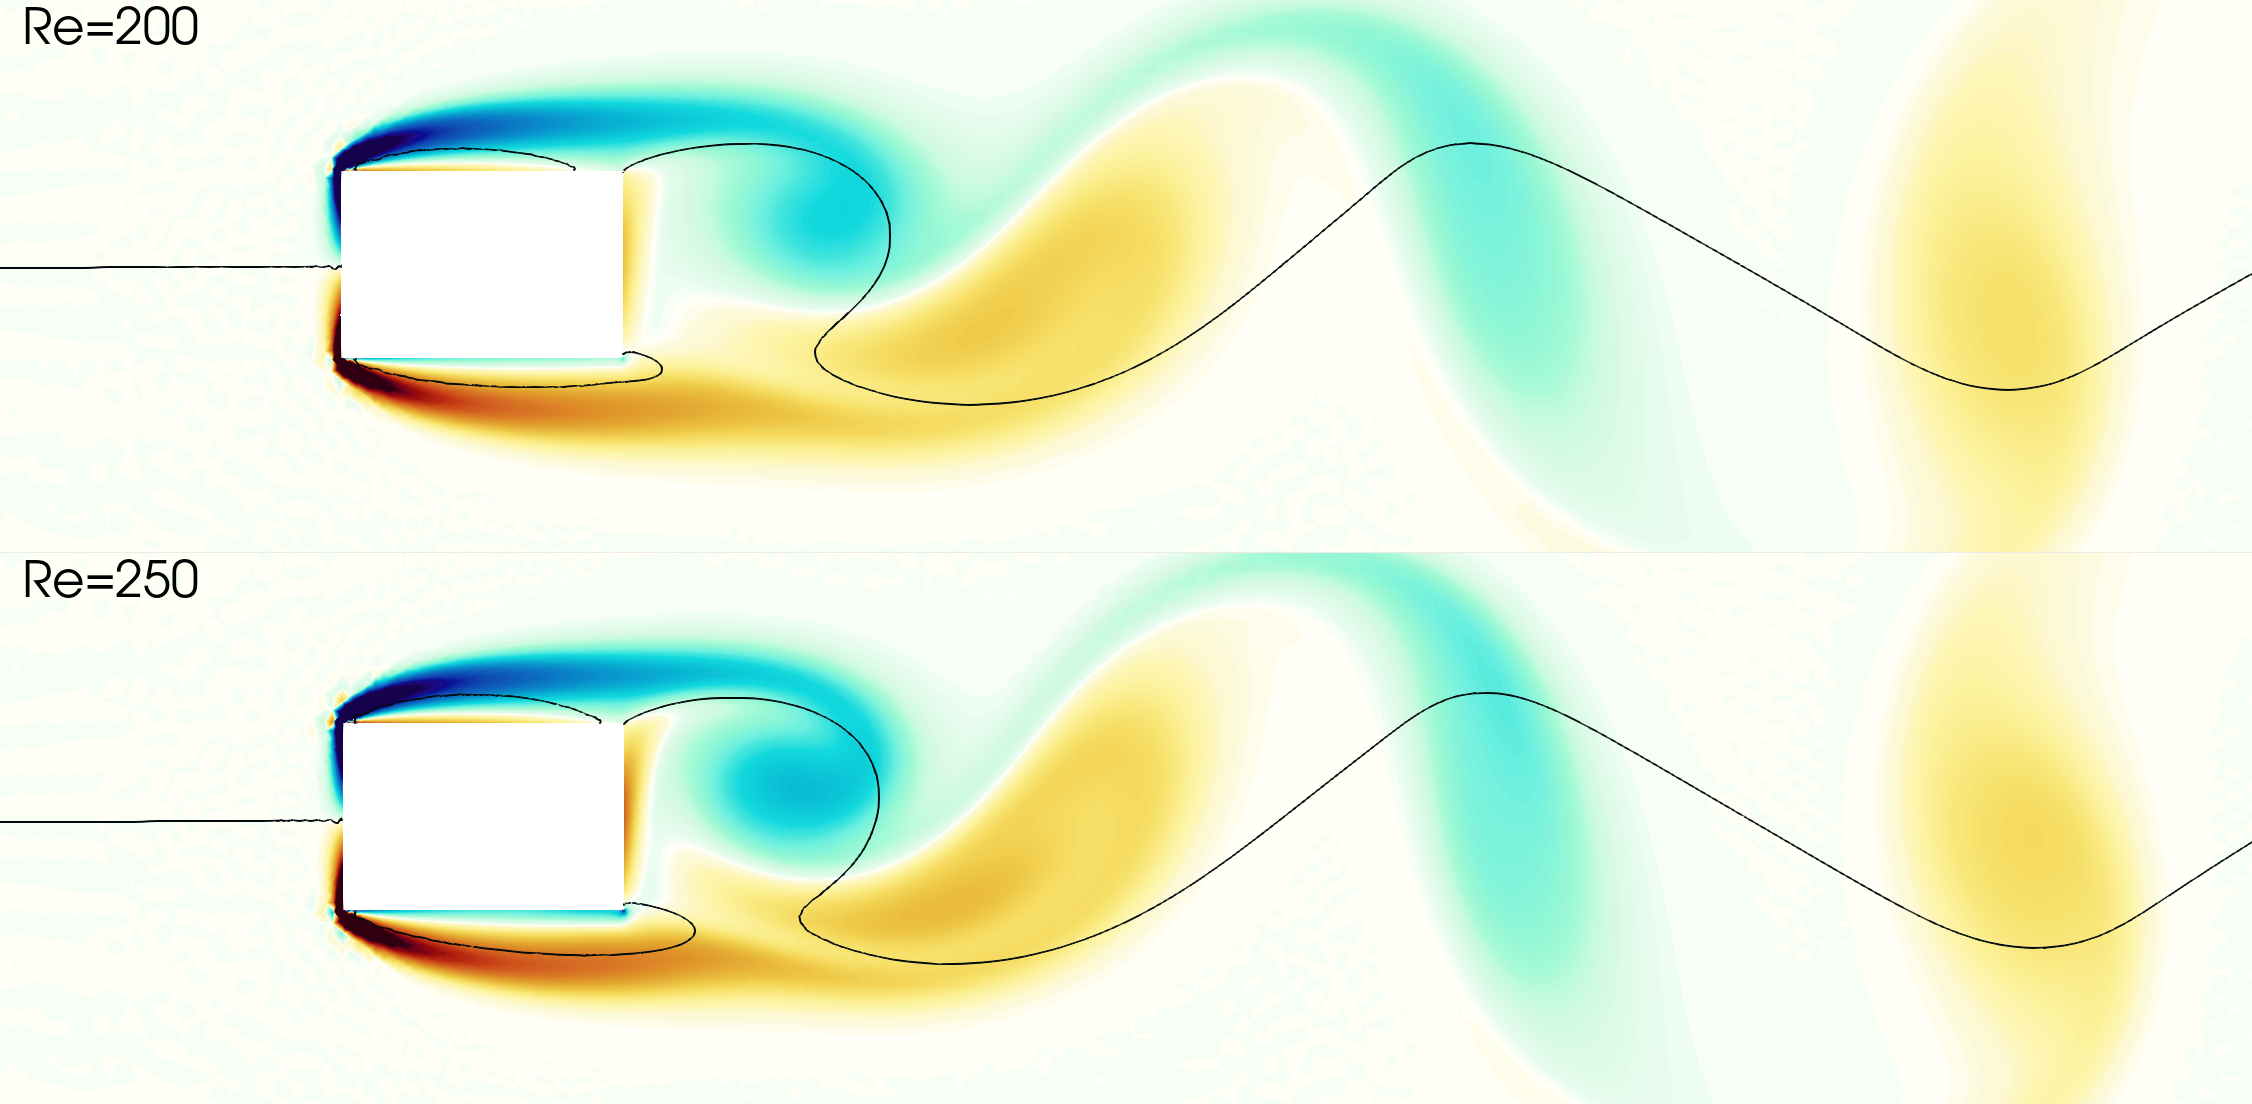
\includegraphics[width=0.49\textwidth]{./fig/AR1p5/snap/snap.0030.png}  
  \caption{Instantaneous snapshots of the base-flow vorticity for $\AR=1$ (top left), $\AR=1.25$ (top right), $\AR=1.5$ (bottom left) and $\AR=1.75$ (bottom right) at $Re=200$ (top) and $Re=250$ (bottom). For all cases the snapshots are taken at the same phase, i.e. just before the shedding of a vortex with negative vorticity in the wake. XX REPLACE $\AR=1.75$ AND ORGANISE THE FIGURE FROM TOP TO BOTTOMXX}
  \label{fig:bf-short}
\end{figure}
%
The influence of $\AR$ on the base-flow topology is shown in figure \ref{fig:bf-short}. For the smaller $\AR < 1.25$, for all considered $Re$ the flow separates at the LE and only rarely reattaches along the lateral sides of the body. In this case the vortex shedding in the wake is thus determined by the dynamics of the LE shear which is indeed active in the formation of the wake vortex. This is visualised in the figure \ref{fig:bf-short} by the streamline separating from the LE that indeed delimits the wake vortex before it is shed in the wake. By contrast, for the larger $\AR>1.25$the LE shear layer (intermittently) reattaches along the lateral sides of the body at all $Re$, and the wake dynamics is mostly determined by the TE shear layer.
For the intermediate $\AR=1.25$ the base-flow topology changes with $Re$. At the lower $Re \le 210$ the flow resembles what has been observed for longer bodies (with the LE shear layer intermittently reattaching along the lateral sides of the body), and the wake vortex shedding is driven by the TE shear layers. At the higher Reynolds numbers ($Re>210$), instead, the flow recovers the low-$\AR$ topology, with the wake dynamics being primarily driven by the LE shear layers. This is visualised in figure \ref{}, when comparing panels xx and xx and noting that the streamline separating at the LE corner reattaches for $Re=200$, but not for $Re=250$. This change of topology is explained with the fact that an increase of $Re$ leads to an increase of the angle with which the flow separates at the LE corners.

\begin{figure}
  \centering
  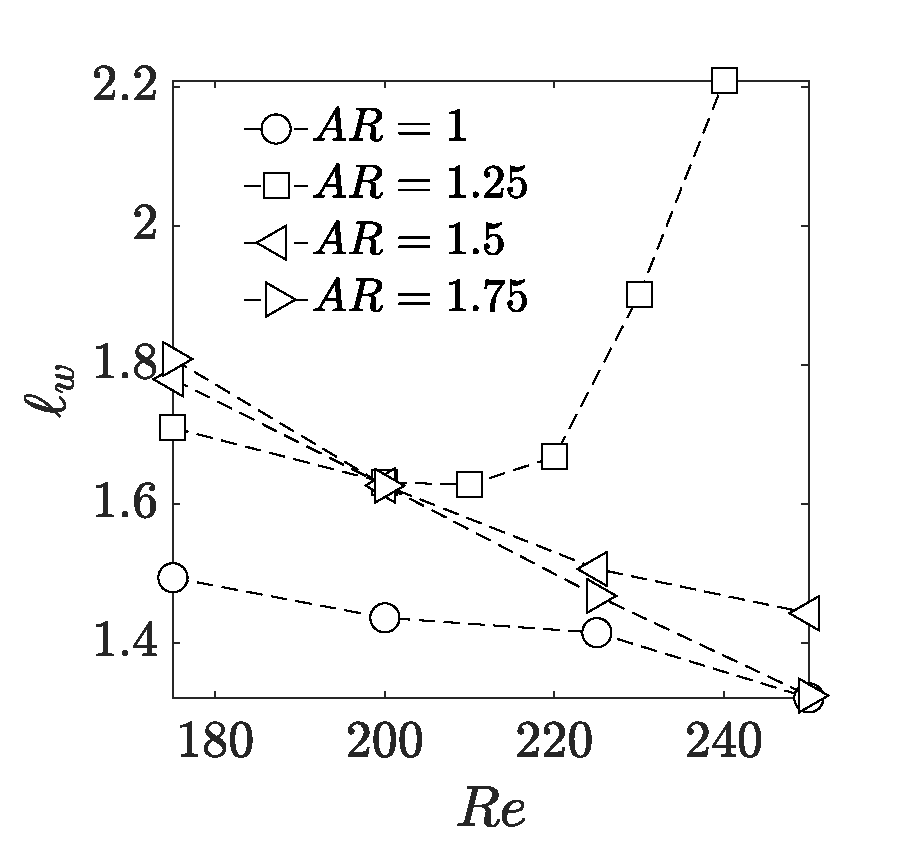
\includegraphics[width=0.32\textwidth]{./fig/AR1s/lw.eps}
  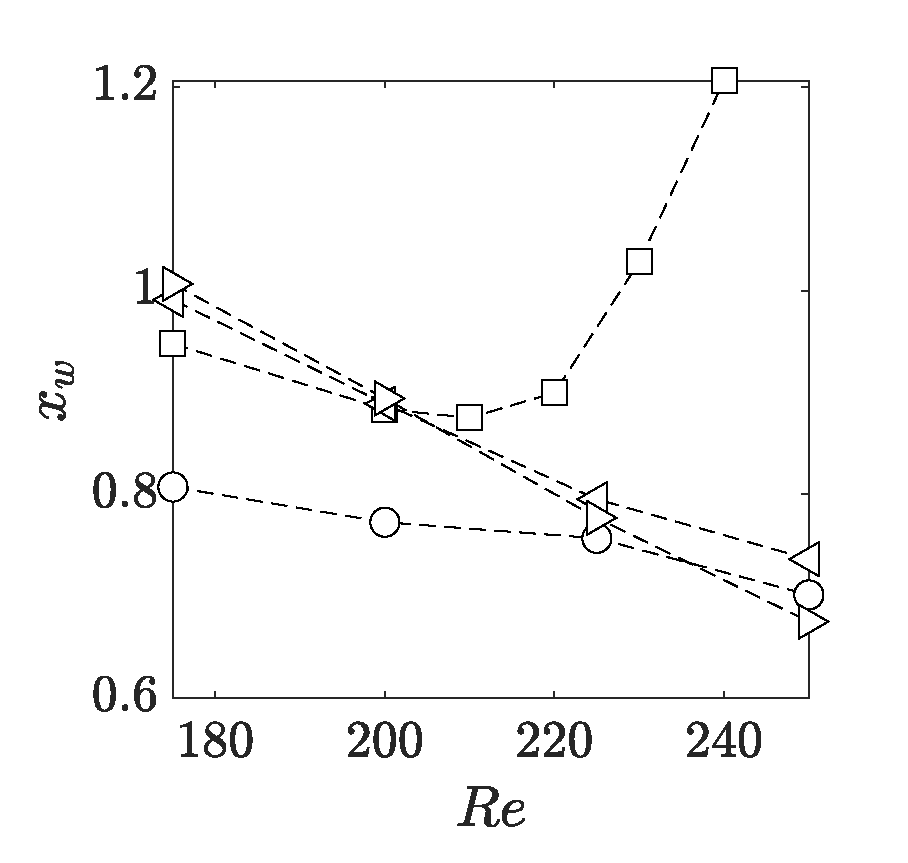
\includegraphics[width=0.32\textwidth]{./fig/AR1s/xw.eps}
  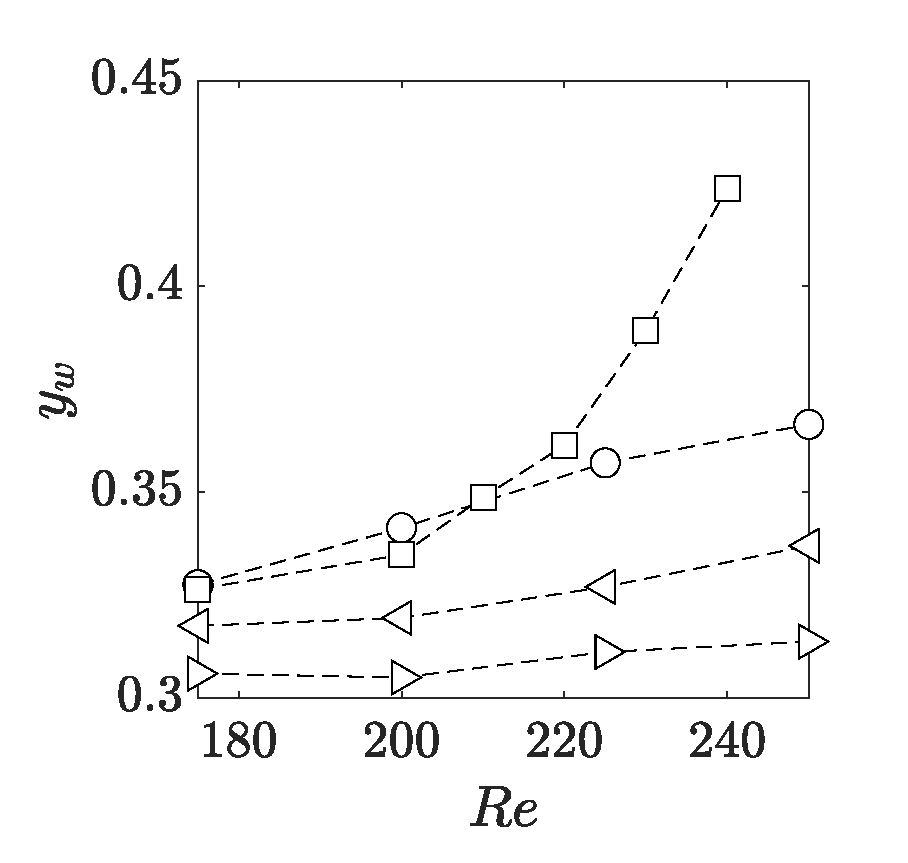
\includegraphics[width=0.32\textwidth]{./fig/AR1s/yw.eps}
  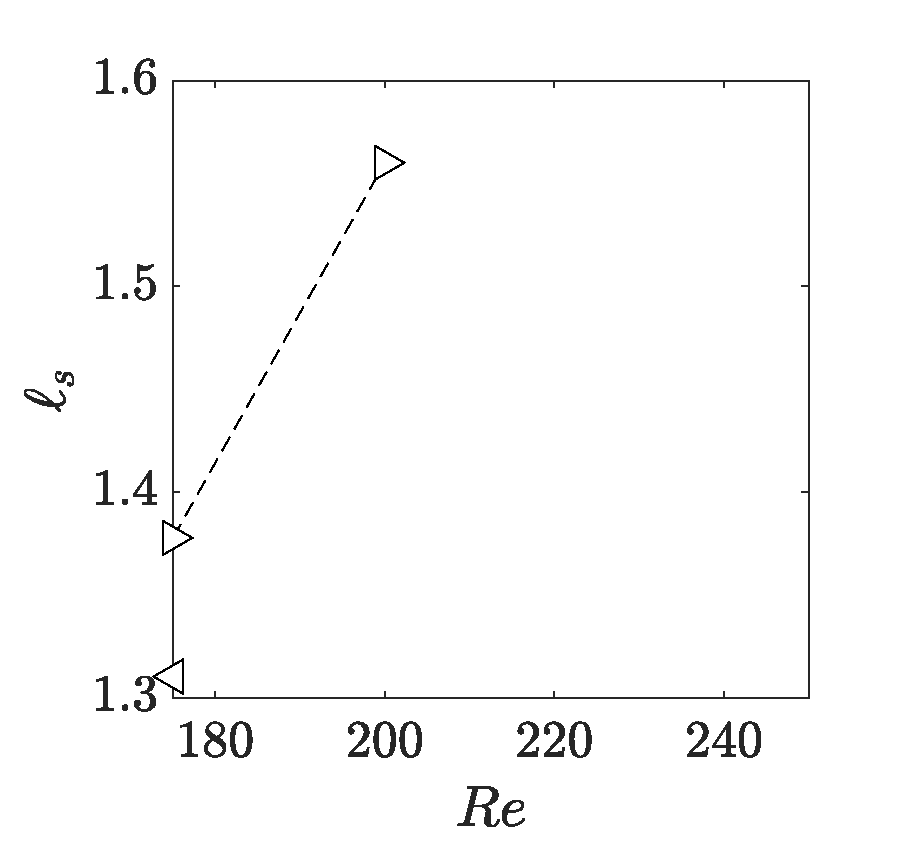
\includegraphics[width=0.32\textwidth]{./fig/AR1s/ls.eps}
  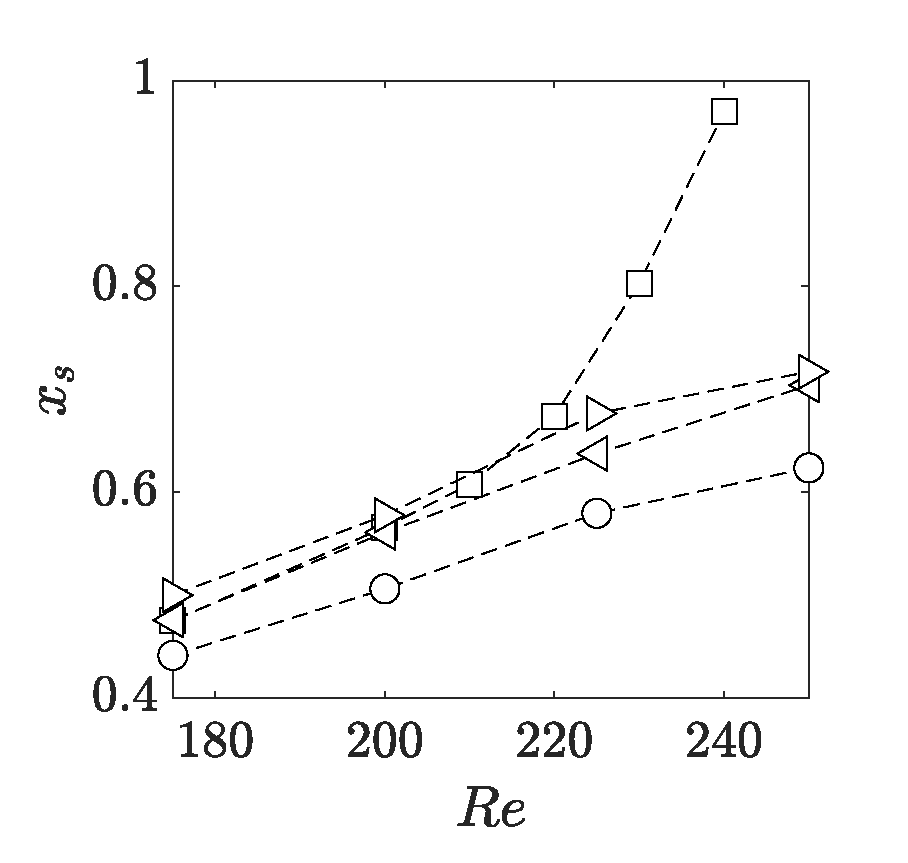
\includegraphics[width=0.32\textwidth]{./fig/AR1s/xs.eps}
  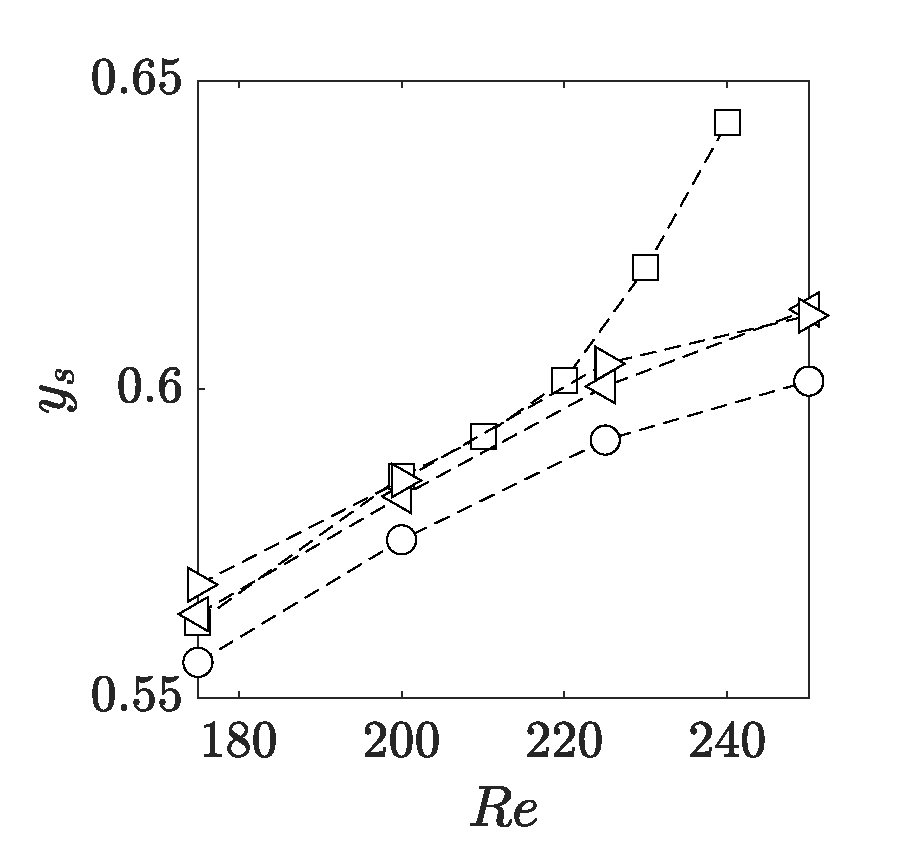
\includegraphics[width=0.32\textwidth]{./fig/AR1s/ys.eps}
  \caption{Dependence of the mean-flow properties on $\AR$ and $Re$ for $1 \le \AR \le 1.75$ and $175 \le Re \le 250$.}
  \label{fig:mf_lengths}
\end{figure}
%
We look at the mean flow averaged over one shedding period; see figure \ref{fig:mf_lengths}. For all $\AR$ an increase of $Re$ leads to an increase of the angle with which the flow separates; see dependence on $Re$ of $y_s$ and $y_w$. As a result the LE shear layers become thicker as $Re$ increases, being thus responsible for the decrease of $\ell_w$. For $\AR=1.25$ the an increase of the Reynolds number leads to a fast increase of $\ell_w$ (and $x_w$) for $Re>210$, which well correlates with the increase of the shedding period. Note that, on average, the flow reattaches along the lateral sides of the body only for $\AR \ge 1.5$ and $Re \le 200$.
% 
\begin{figure}
  \centering
  \includegraphics[width=0.49\textwidth]{./fig/AR1/LinStab/sens_Re200.eps}
  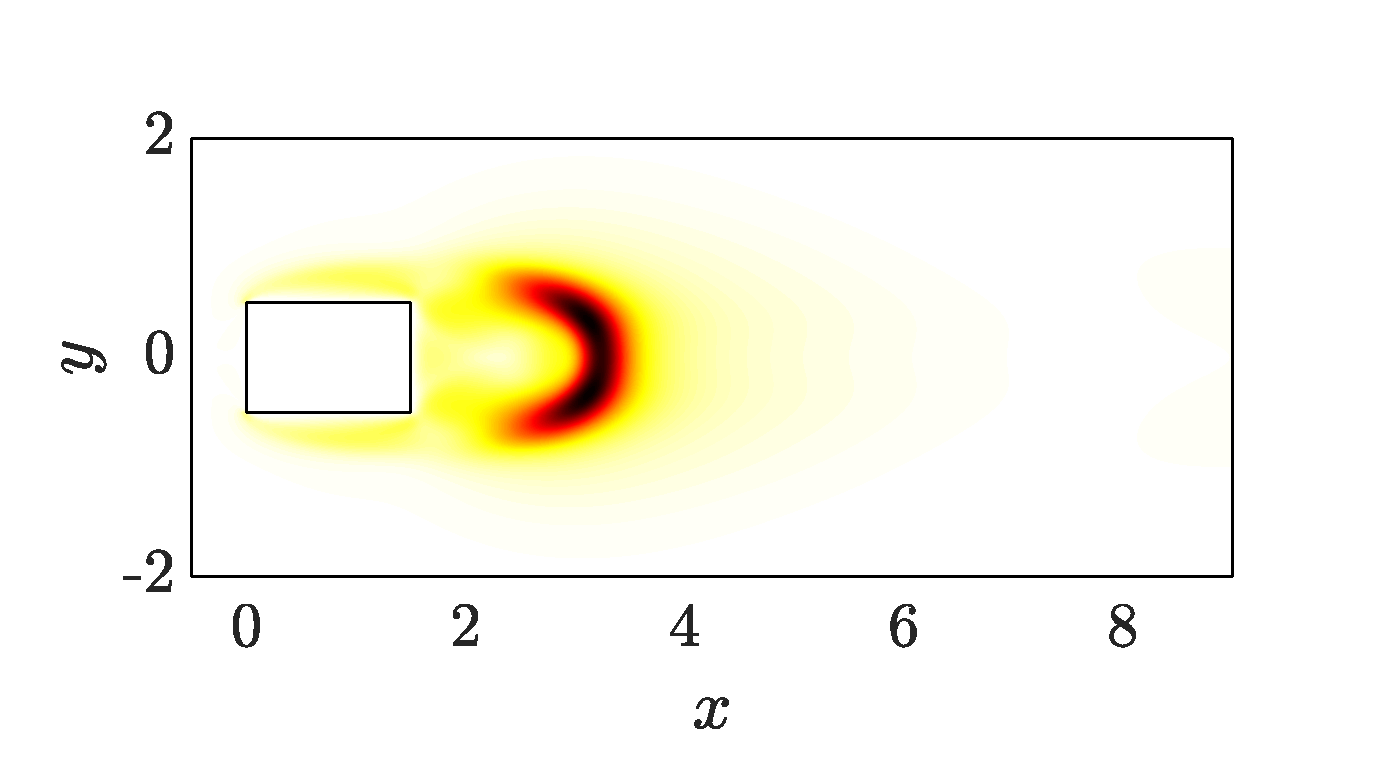
\includegraphics[width=0.49\textwidth]{./fig/AR1p5/LinStab/sens_Re200.eps}
  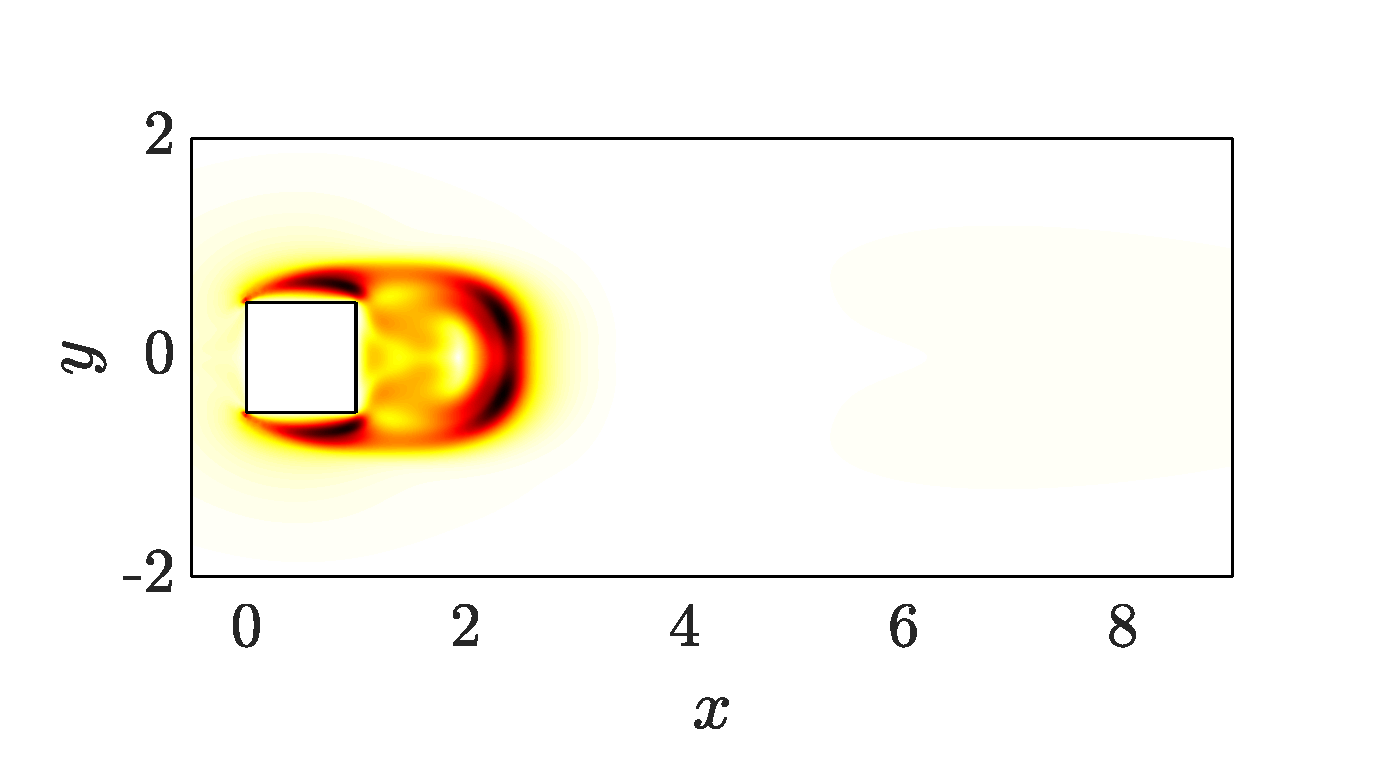
\includegraphics[width=0.49\textwidth]{./fig/AR1/LinStab/sens_Re250.eps}
  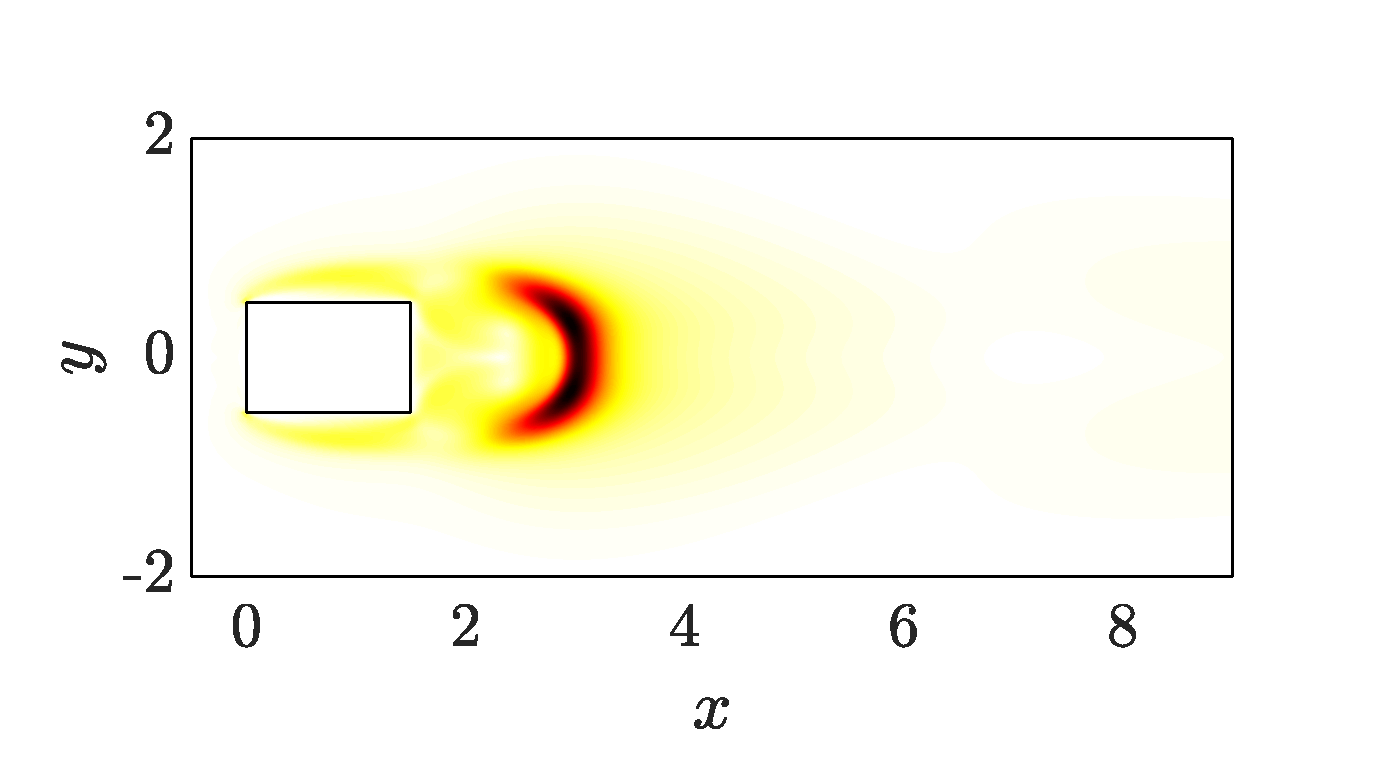
\includegraphics[width=0.49\textwidth]{./fig/AR1p5/LinStab/sens_Re250.eps}
  \includegraphics[width=0.49\textwidth]{./fig/AR1p25/LinStab/sens_Re200.eps}
  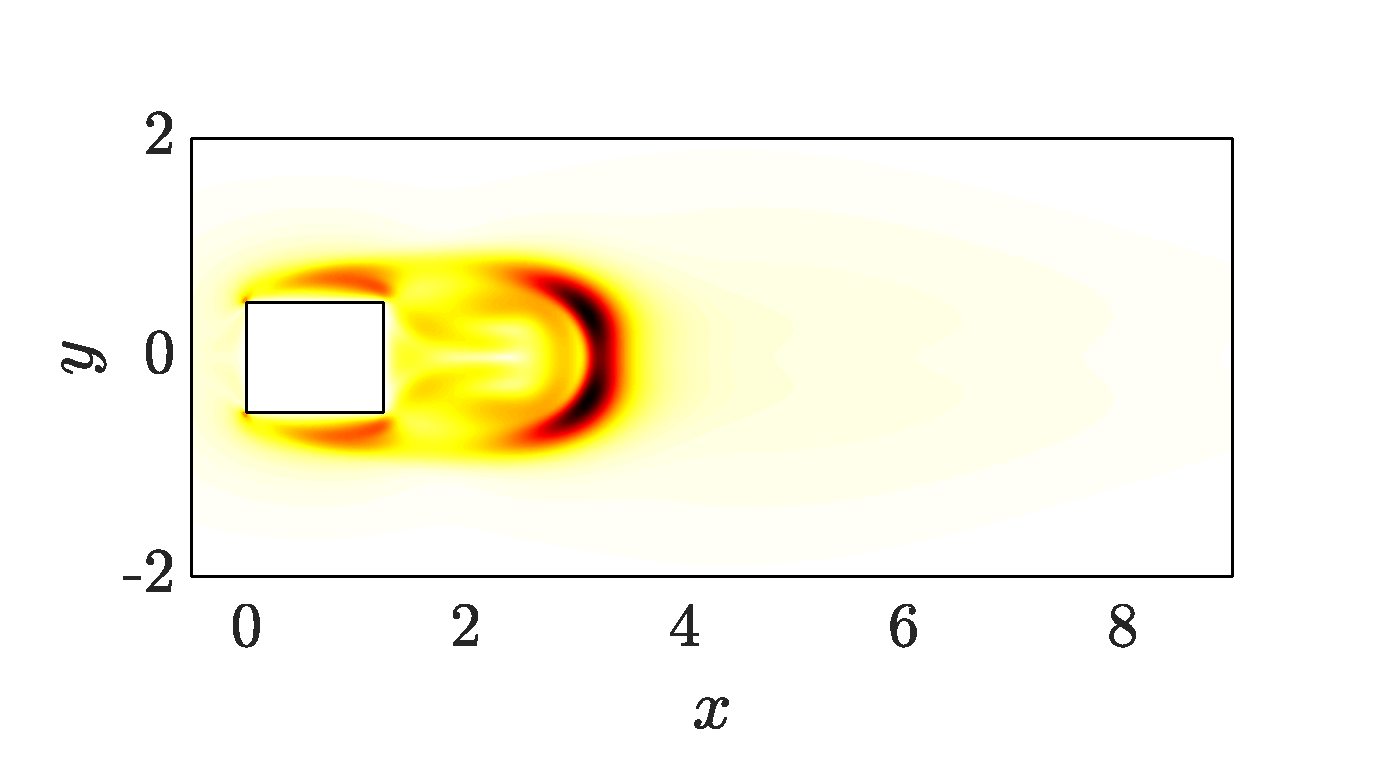
\includegraphics[width=0.49\textwidth]{./fig/AR1p25/LinStab/sens_Re230.eps}
  \caption{Linear stability analysis of the mean fow for $\AR=1$ and $Re=200$ (top left), $\AR=1.5$ and $Re=200$ (top right), $\AR=1$ and $Re=250$ (centre left), $\AR=1.5$ and $Re=250$ (centre right) $\AR=1.25$ and $Re=200$ (bottom left) and $\AR=1.25$ and $Re=230$ (bottom right).}
  \label{fig:mf_sens}
\end{figure}
%
To further highlight the change of the flow topology with $\AR$ and $Re$, we perform a global stability analysis of the mean flow averaged over one shedding period. The focus in on the leading eigenmode, which is representative of the unsteady phenomena of the flow. For a similar approach see for example \cite{pier-2002,barkley-2006} for the circular cylinder and \cite{chiarini-quadrio-auteri-2022} for rectangular cylinders. 

The frequency of the leading eigenmode predicts fairly well the Strouhal number observed in the nonlinear simulations for all cases, with a maximum difference of $xx\%$. Unlike the case of the circular cylinder, which is marignally stably \citep{barkley-2006}, the present mean flow stability analysis leads to a slightly negative growth rate. Figure \ref{fig:mf_sens}, shows the structural sensitivity of the leading mode. The structural sensitivity was introduced by \cite{giannetti-luchini-2007} as an upper bound for the eigenvalue variation induced by a specific perturbation of the linearised Navier--Stokes operator, namely a `force-velocity coupling' representing feedback from a localised velocity sensor to a localised force actuator at the same location. In this sense, the structural sensitivity in as indicator of the eigenvalue sensitivity and identifies the wavemaker \citep{monkewitz-etal-1993}. The structural sensitivity identifies the flow region where structural modifications of the stability problem produce the strongest drift of the leading eigenvalue and indentifies the so-called wavemaker. The largest values of the sensitivity occur near the cylinders, as the product of the adjoint and direct modes is small in the remaining part of the domain. For longer bodies and smaller $Re$ non null values are observed only in the wake behind the TE along the streamline delimiting the mean recirculating region. The core of the instability responsible for the TE vortex shedding is located downstream the TE. For shorter bodies and/or larger $Re$ the structural sensitivity is non negligible also along the LE shear layers over the lateral sides of the cylinder. Accordingly, in these cases the wavemaker extends to the LE shear layers, as they play a role inthe wave vortex shedding dyanmics.
\fi

\subsection{The bifurcations}

\begin{figure}
  \centering
  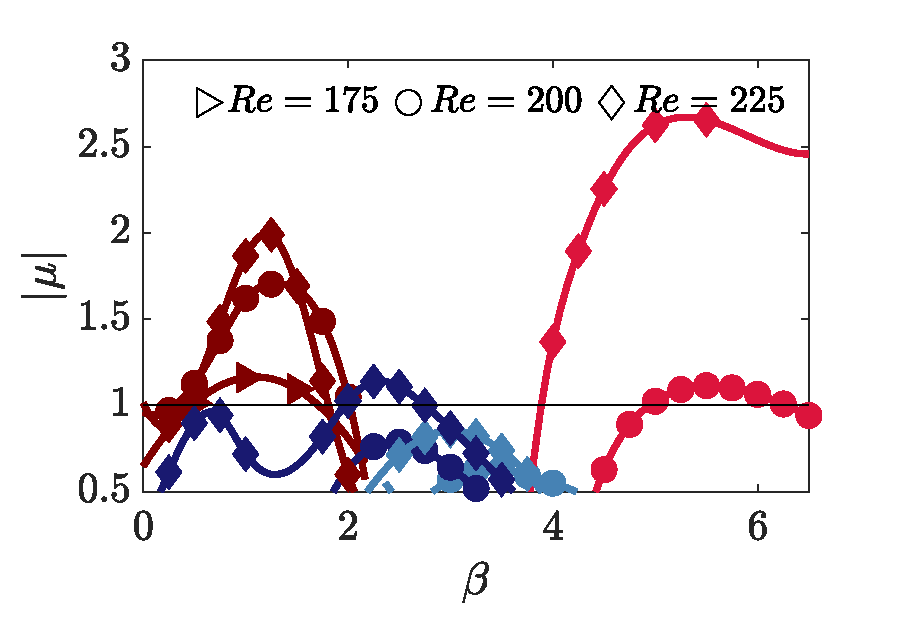
\includegraphics[width=0.49\textwidth]{./fig/AR1/neutralb.eps}
  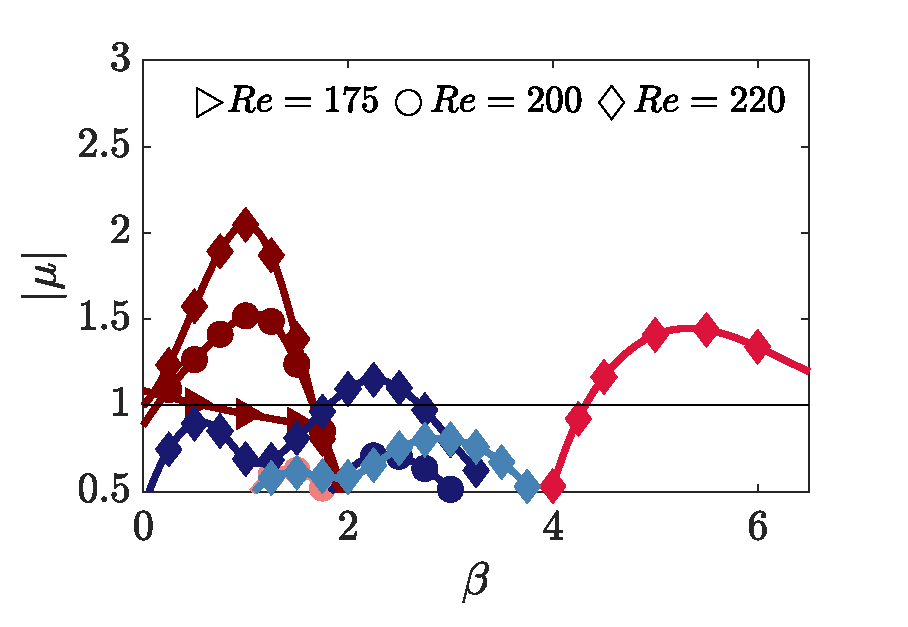
\includegraphics[width=0.49\textwidth]{./fig/AR1p25/neutralb.eps}  
  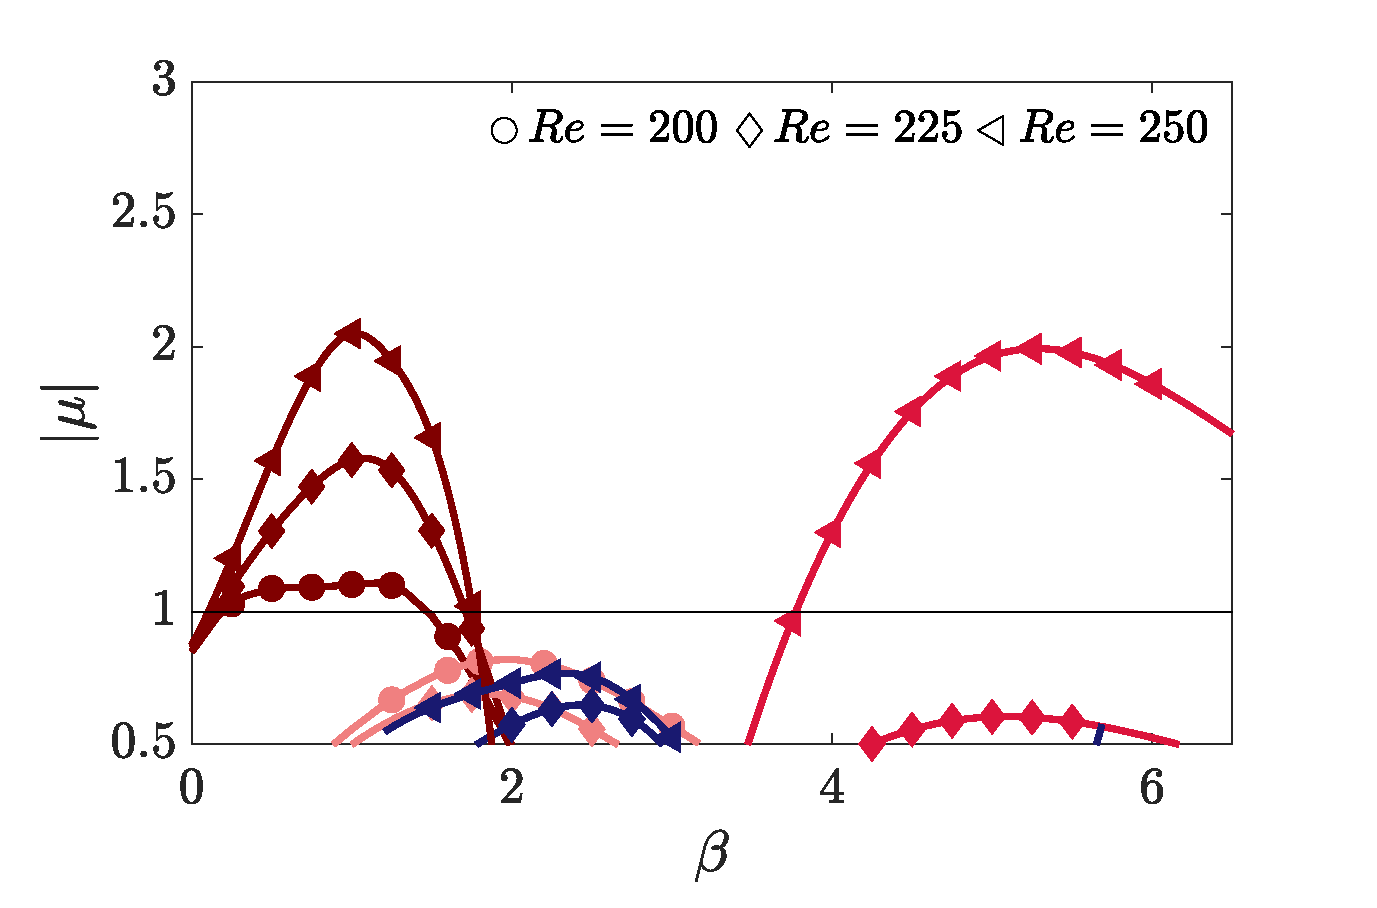
\includegraphics[width=0.49\textwidth]{./fig/AR1p5/neutralb.eps}    
  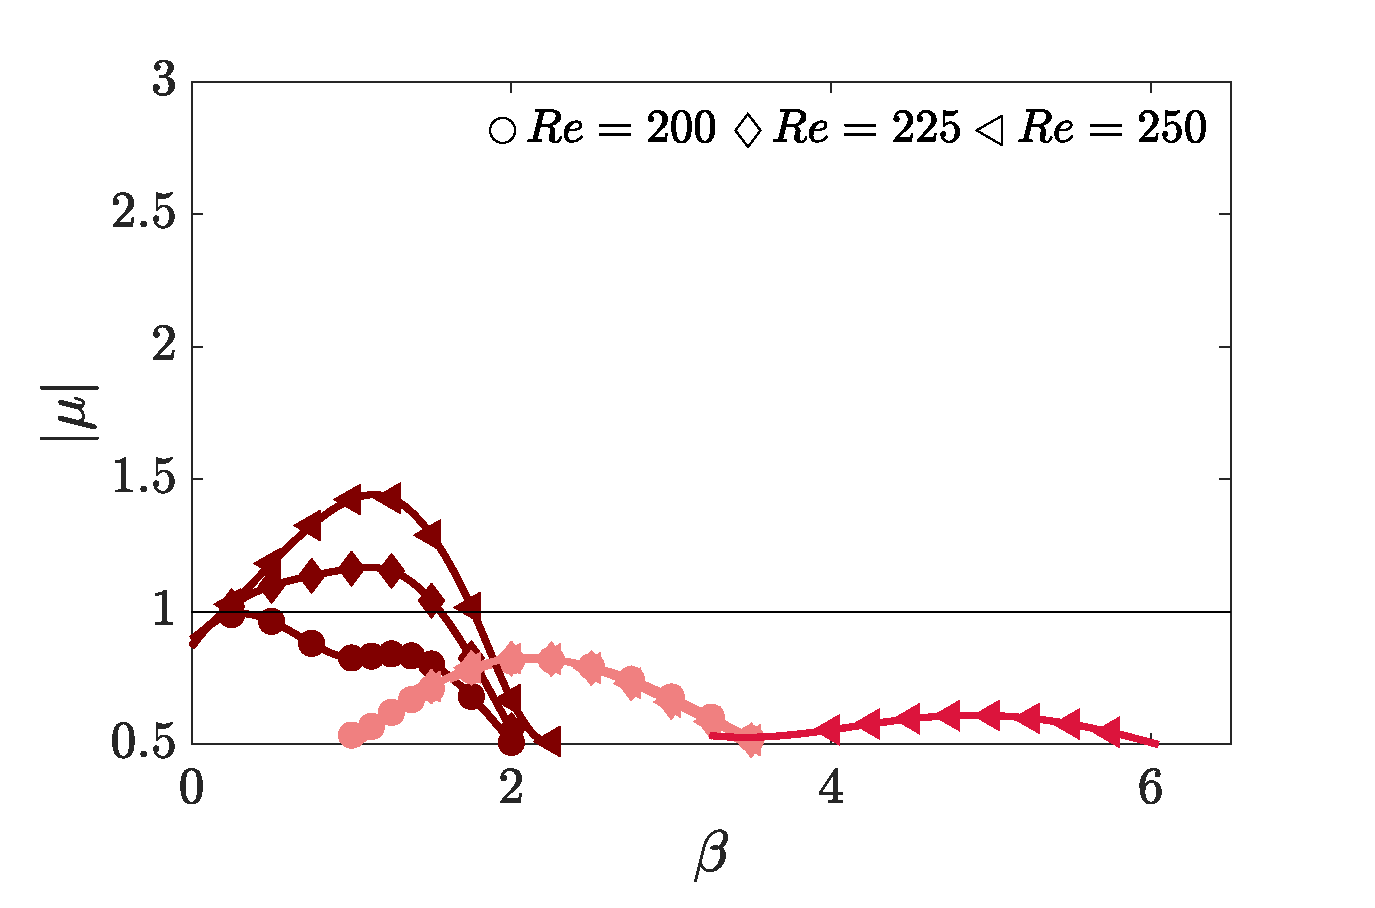
\includegraphics[width=0.49\textwidth]{./fig/AR1p75/neutralb.eps}       
  \caption{Multipliers for $\AR=1$ (top left), $\AR=1.25$ (top right), $\AR=1.5$ (bottom left) and $\AR=1.75$ (bottom right) for different $Re$. The dark red line refers to mode $A$, the light blue line to mode $C$, the light red to mode $B$, the dark blue lines to mode $QP$, the light blue line refers to mode $B'$, and pink lines mode $C$. Mode $B'$ has the same spatio-temporal symmetry of mode $B$, but its characteristic wavelength is much smaller, being similar to that of mode $A$. This mode resembles that found for elongated bodies with elliptic leading edge by \cite{ryan-etal-2005}. XX ADD $\AR=2$ e $\AR=2.5$ XX}
  \label{fig:mult_AR1_AR1p75}
\end{figure}
%
\begin{figure}
  \centering
  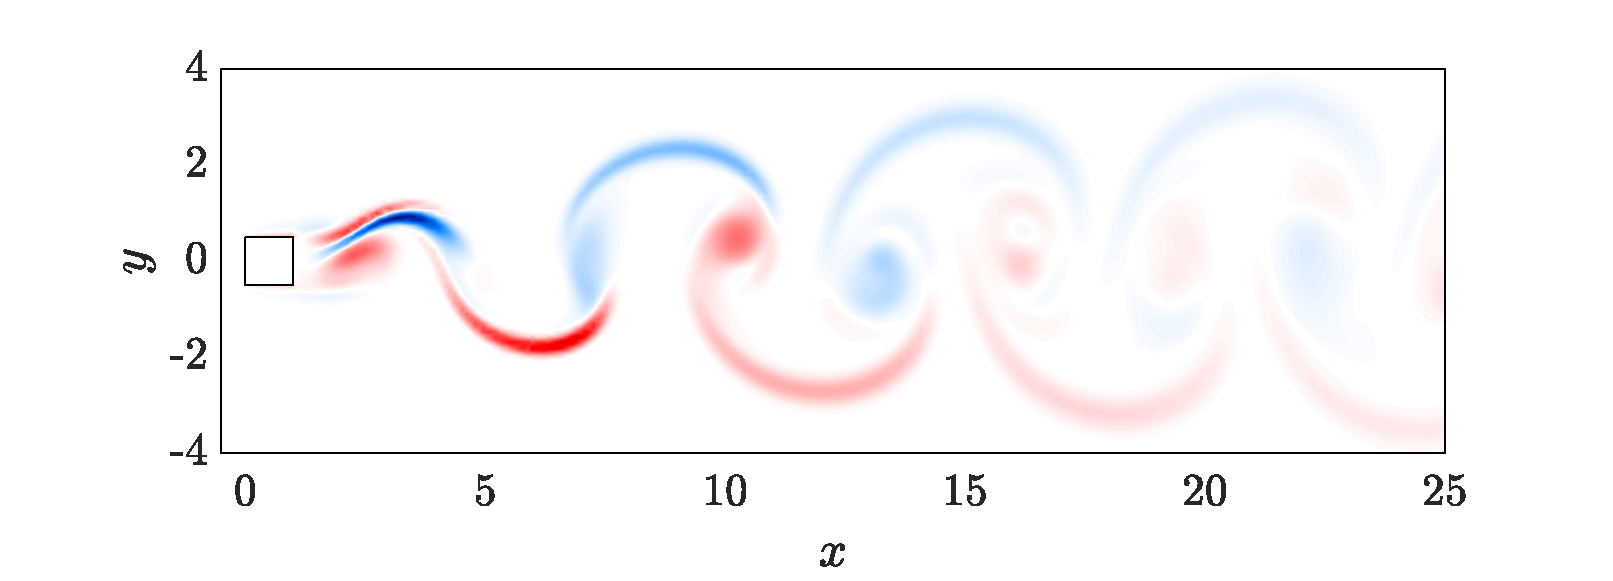
\includegraphics[width=0.49\textwidth]{./fig/AR1/omegax_Re200_beta_1p5_modeA.eps}
  \includegraphics[width=0.49\textwidth]{./fig/AR1p25/omegax_Re200_beta_5p5_modeB.eps}
  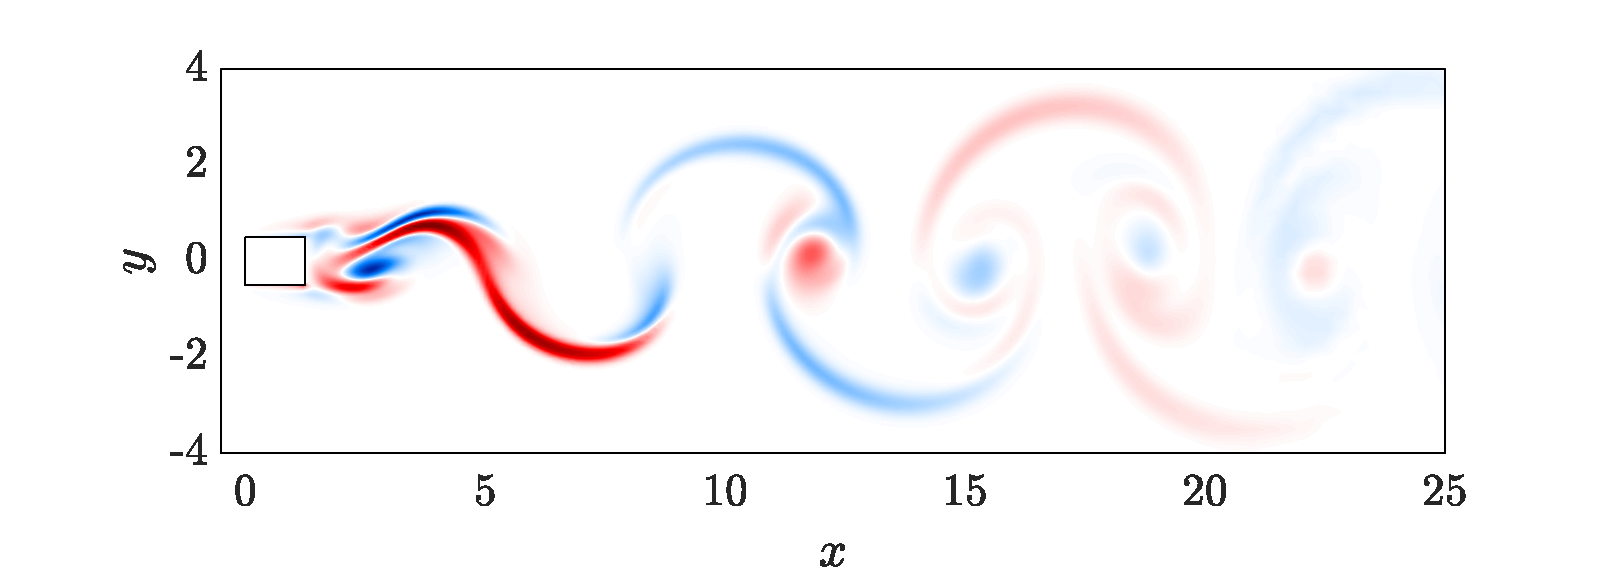
\includegraphics[width=0.49\textwidth]{./fig/AR1p25/omegax_Re230_beta_2p25_modeC.eps}
  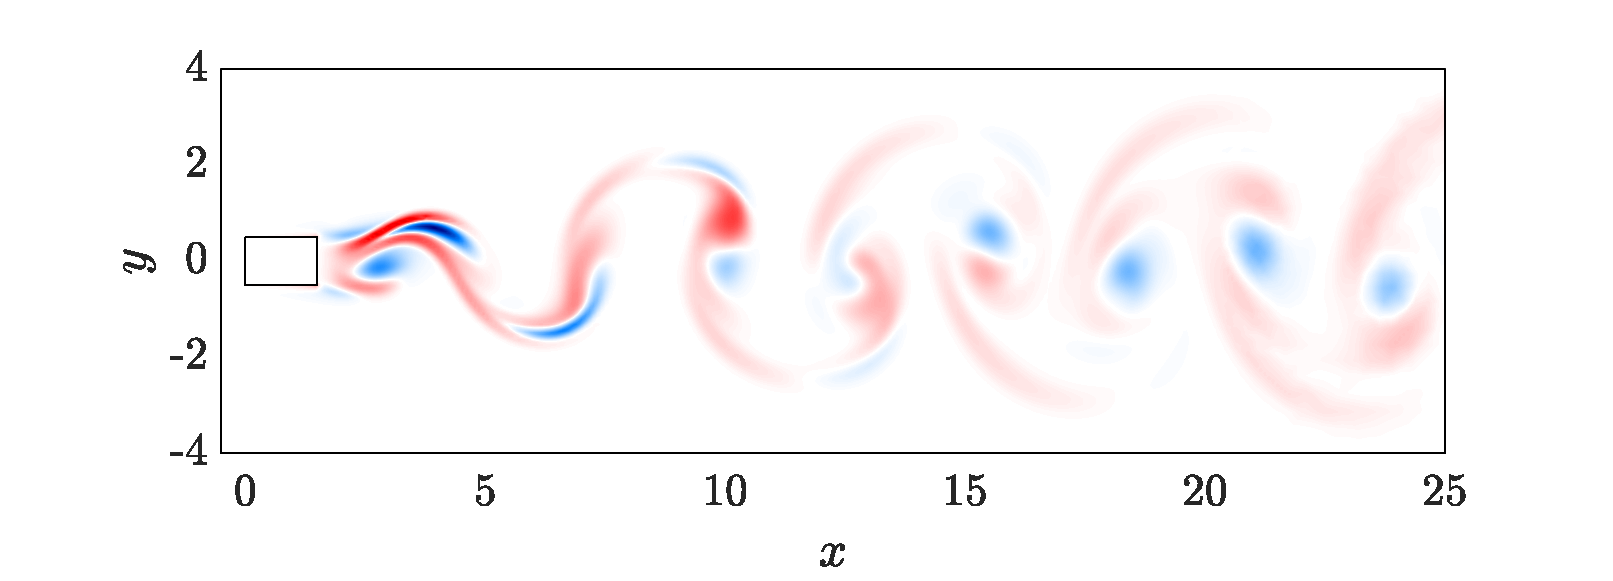
\includegraphics[width=0.49\textwidth]{./fig/AR1p5/omegax_Re200_beta_2p2_modeBp.eps}
  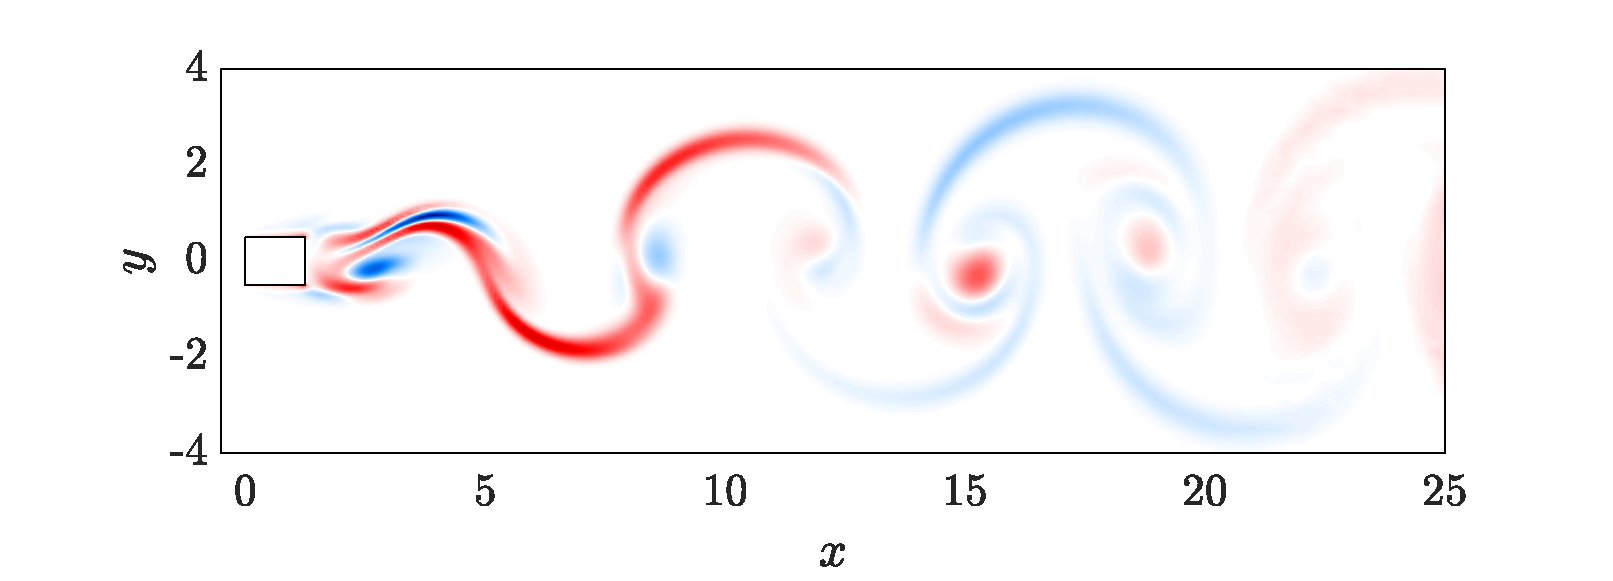
\includegraphics[width=0.49\textwidth]{./fig/AR1p25/omegax_Re230_beta_2p25_modeD.eps}
  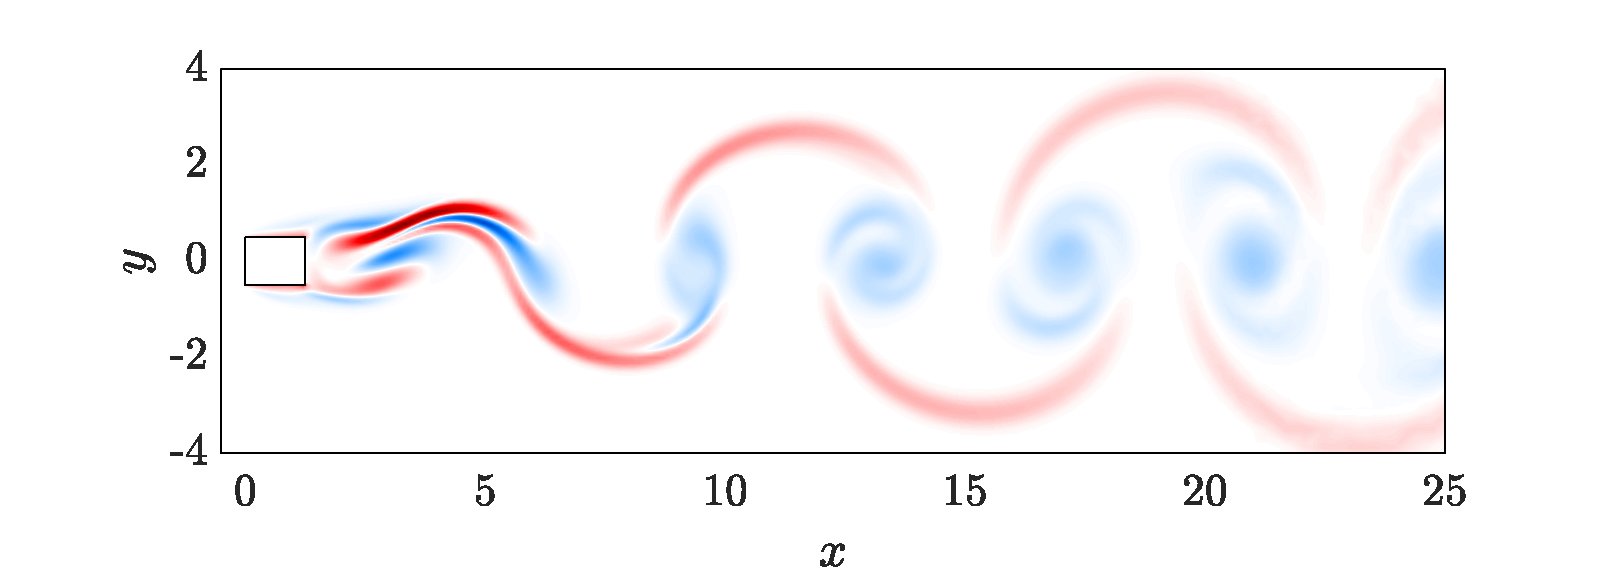
\includegraphics[width=0.49\textwidth]{./fig/AR1p25/omegax_Re240_beta_0p5_modeBpp.eps}
  \caption{Spatial structure of the modes for $1 \le AR \le 1.75$ and $175 \le Re \le 250$. Top left: mode A for $\AR=1$, $Re=200$ and $\beta=1.5$. Top right: mode B for $\AR=1.25$, $Re=200$ and $\beta=5.5$. Centre left: mode QP for $\AR=1.25$, $Re=230$ and $\beta = 2.25$. Centre right: mode $B'$ for $\AR=1.5$, $Re=200$ and $\beta=2.2$. Bottom left: mode QP' for $\AR=1.25$, $Re=230$ and $\beta=2.25$. Bottom right: mode B'' for $\AR=1.25$, $Re=240$ and $\beta=0.5$.}
  \label{fig:modes}
\end{figure}
%
As discussed in \S\ref{sec:intro}, for $\AR=1$, three distinct modes become unstable in rapid succession as the Reynolds number increases. Mode $A$ is the first to become unstable, at $Re \approx 175$, with a characteristic wavelength $\lambda_A \approx 5$ (corresponding to $\beta_A \approx 1.2$). This mode exhibits the following spatio-temporal symmetry:
%
\begin{equation}
\begin{aligned}
\hat{u}(x,y,\beta,t) = &+ \hat{u}(x,-y,\beta,t+T/2) \nonumber \\
\hat{v}(x,y,\beta,t) = &-\hat{v}(x,-y,\beta,t+T/2) \nonumber \\
\hat{w}(x,y,\beta,t) = &+ \hat{w}(x,-y,\beta,t+T/2),
\end{aligned}
\end{equation}
%
which leads to an antisymmetric streamwise vorticity:
%
\begin{equation}
\hat{\omega}_x(x,y,\beta,t) = -\hat{\omega}_x(x,-y,\beta,t+T/2).
\end{equation}

Mode B becomes unstable at $Re \approx 200$, with a much shorter characteristic wavelength $\lambda_B \approx 1$ (corresponding to $\beta_B \approx 5.8$). It satisfies a similar symmetry in the streamwise and cross-stream components, but differs in the spanwise component:
%
\begin{equation}
\begin{aligned}
\hat{u}(x,y,\beta,t) = &+\hat{u}(x,-y,\beta,t+T/2), \nonumber \\
\hat{v}(x,y,\beta,t) = &-\hat{v}(x,-y,\beta,t+T/2), \nonumber \\
\hat{w}(x,y,\beta,t) = &-\hat{w}(x,-y,\beta,t+T/2),
\end{aligned}
\end{equation}
%
resulting in a symmetric streamwise vorticity:
%
\begin{equation}
\hat{\omega}_x(x,y,\beta,t) = +\hat{\omega}_x(x,-y,\beta,t+T/2).
\end{equation}

Finally, Mode QP becomes unstable at the higher Reynolds number $Re \approx 230$, with an intermediate characteristic wavelength of $\lambda_{QP} \approx 2.7$ (corresponding to $\beta_{QP} \approx 2.3$).
%
These results are in excellent agreement with our numerical predictions shown in figures~\ref{fig:mult_AR1_AR1p75}$(a)$ and~\ref{fig:modes}, providing a validation of the computational methodology.

Figure~\ref{fig:mult_AR1_AR1p75}(b-d) illustrates the effect of increasing aspect ratio. As $\AR$ increases, the onset of secondary instabilities is progressively delayed. At fixed $Re$, we observe a consistent reduction in the modulus of the Floquet multipliers associated with the three modes, indicating that the base flow becomes more stable for longer bodies. Quantitatively, the critical Reynolds number increases from $Re_{c2} \approx 175$ for $\AR=1$ to approximately $Re_{c2} = 200-225$ for $\AR=1.75$. This trend is consistent with the delayed onset of the primary instability reported by \citet{chiarini-quadrio-auteri-2021} for increasing $\AR$.

Despite the stabilising effect of elongation, the sequence of bifurcations remains unchanged for $1 \le \AR \le 1.5$, with mode $A$ becoming unstable first, followed by mode $B$. However, mode $QP$ is not detected for $\AR>1.5$ within the range of Reynolds numbers investigated. The characteristic wavelengths of modes $A$ and $B$ exhibit only minor variations with aspect ratio, consistent with the findings of \cite{choi-yang-2014} for $\AR<1$.

In addition to the three established modes, a new mode---denoted $B'$---emerges for $\AR>1$. Mode $B'$ shares the same spatio-temporal symmetry as mode $B$, but has a significantly longer wavelength, comparable to that of mode $A$, see figure~\ref{fig:modes_AR1_AR1p75}. A mode with similar features---both in wavelength and symmetry---was previously reported by \cite{ryan-etal-2006} in the wake of elongated bodies with streamlined leading edges and blunt trailing edges. Within the parameter range considered here, mode $B'$ remains stable for all configurations.

\begin{figure}
  \centering
  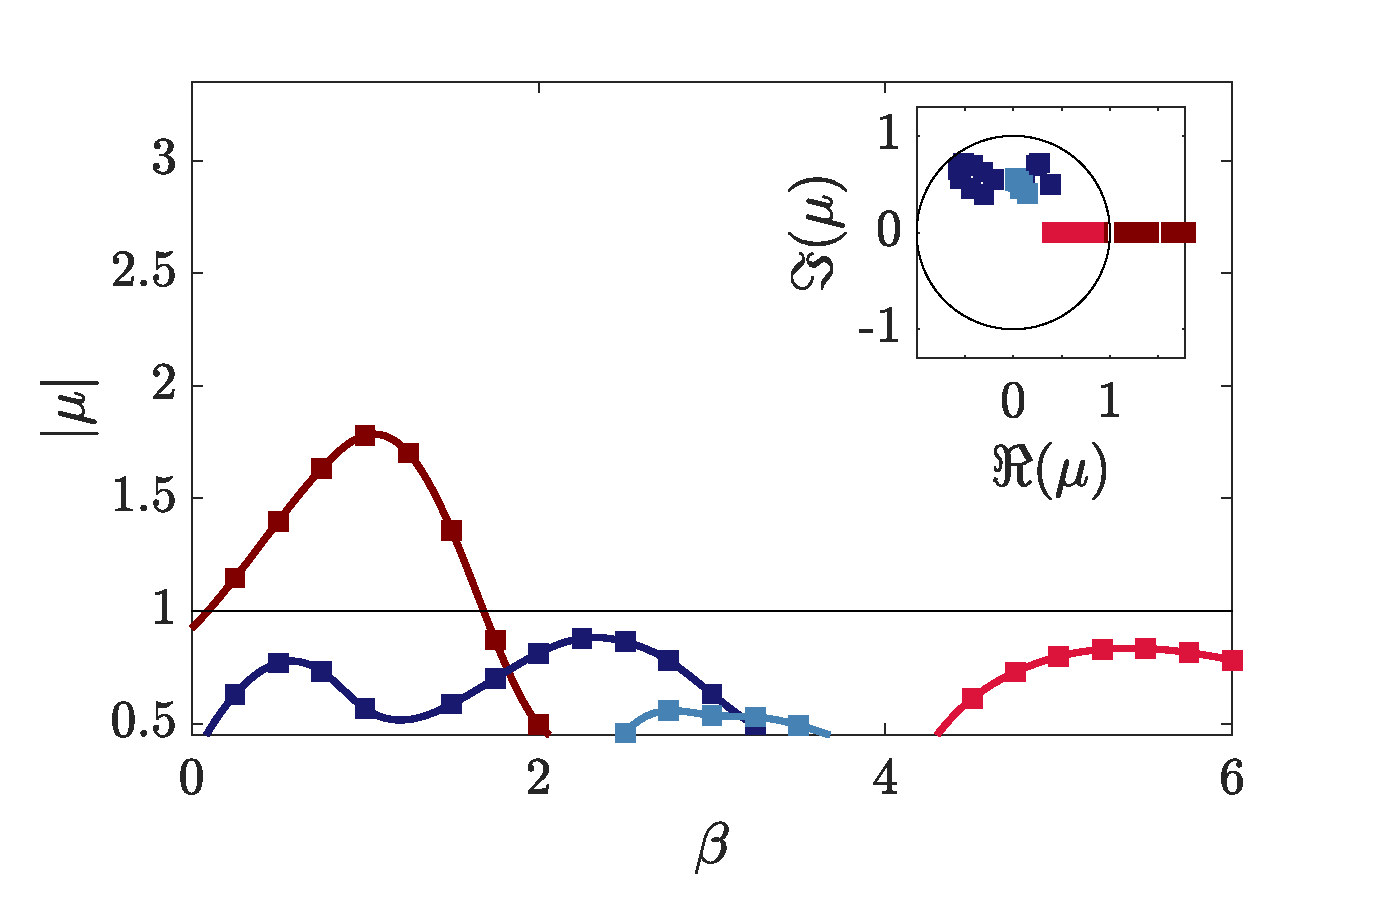
\includegraphics[width=0.49\textwidth]{./fig/AR1p25/mu_beta_Re210.eps}
  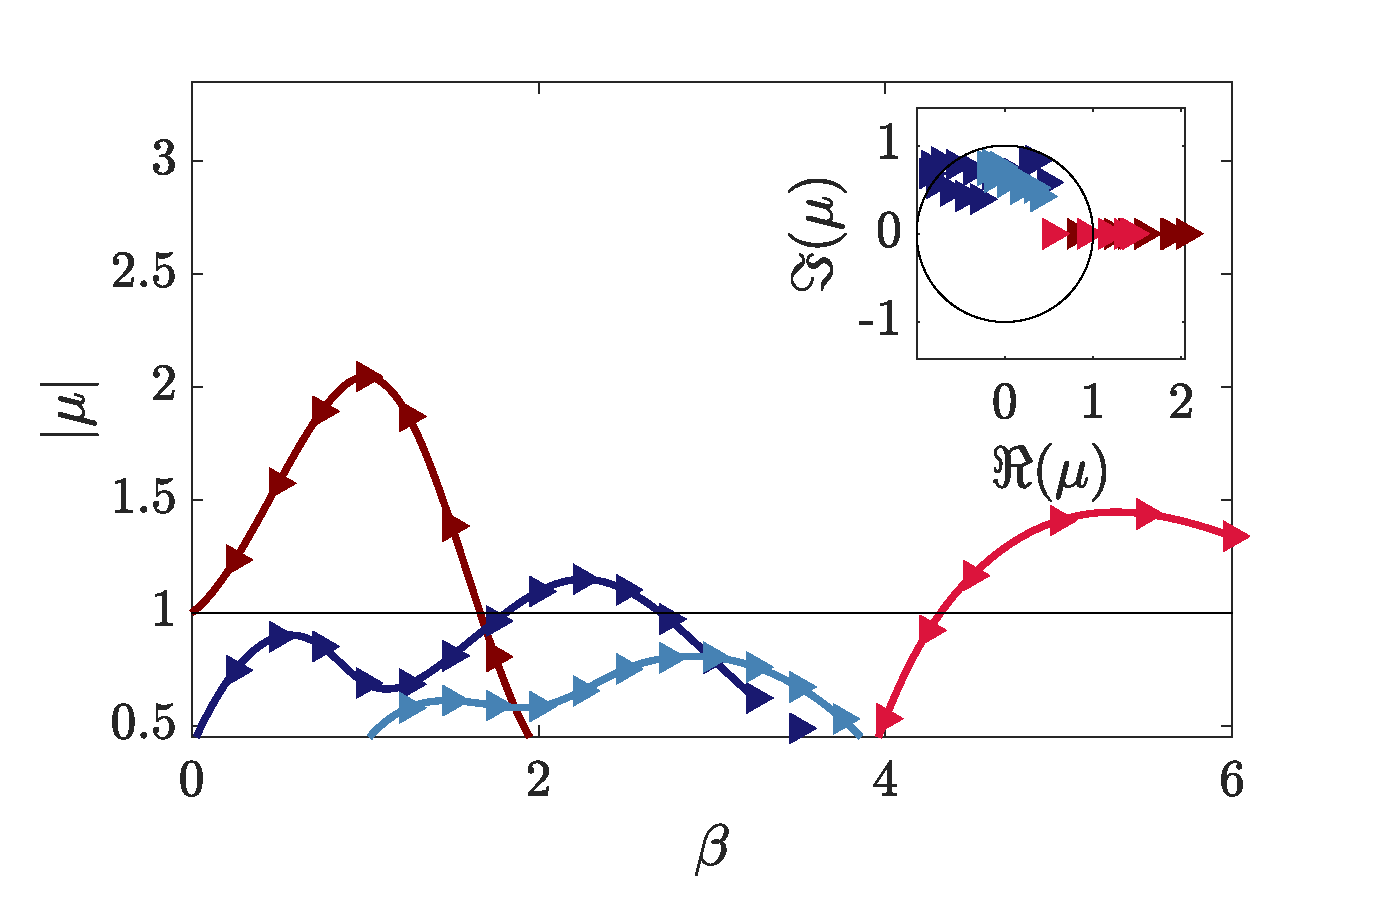
\includegraphics[width=0.49\textwidth]{./fig/AR1p25/mu_beta_Re220.eps}
  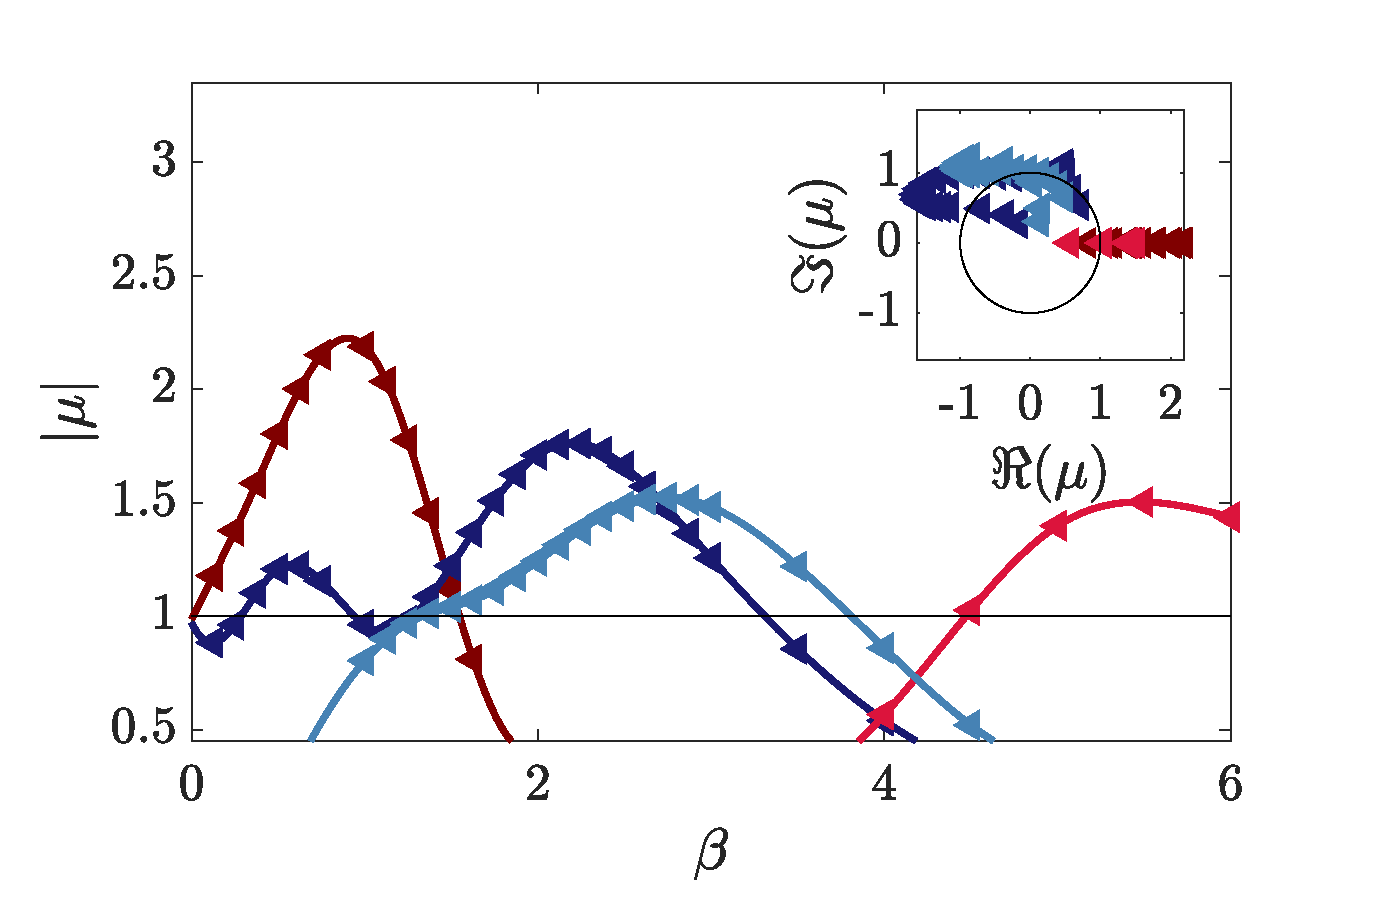
\includegraphics[width=0.49\textwidth]{./fig/AR1p25/mu_beta_Re230.eps}
  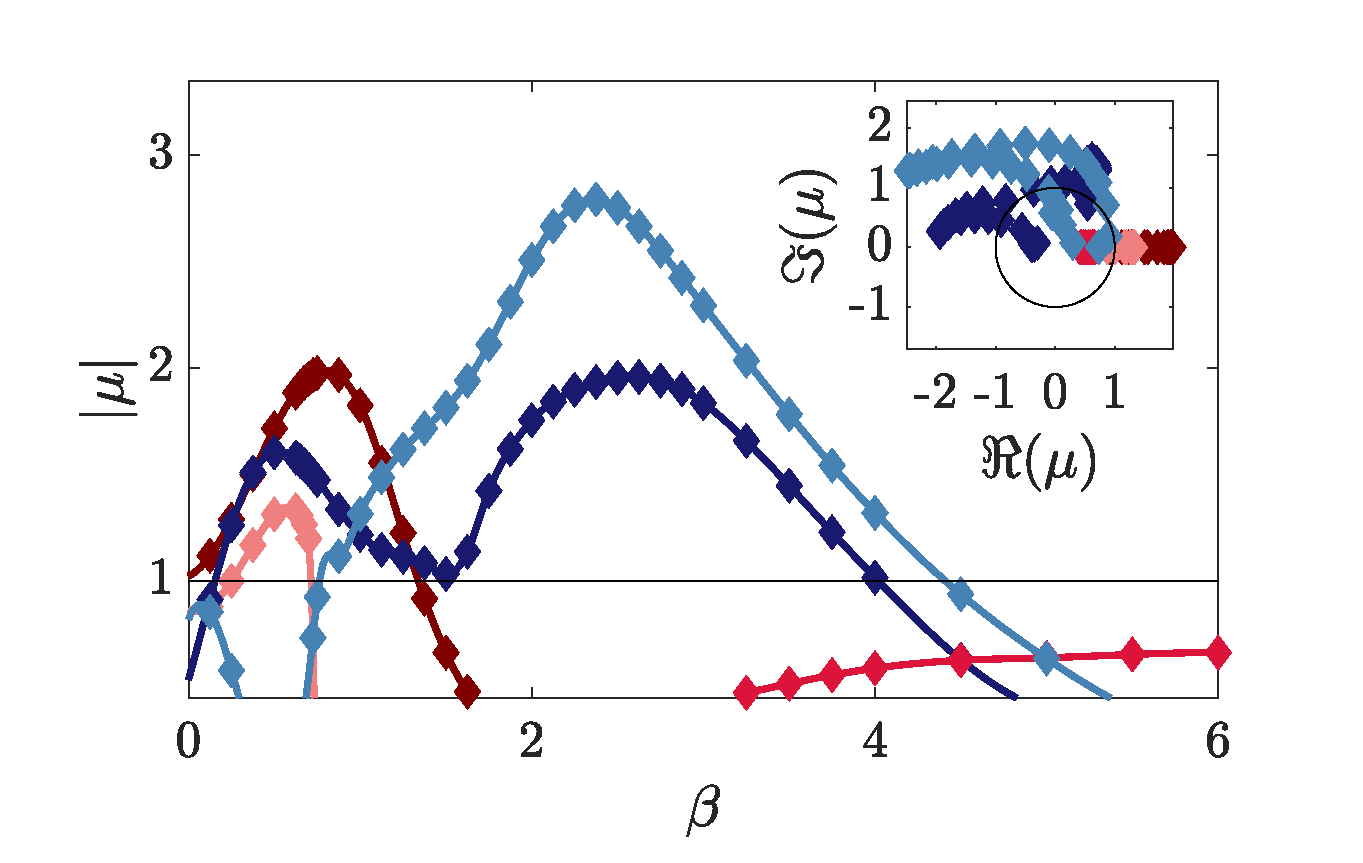
\includegraphics[width=0.49\textwidth]{./fig/AR1p25/mu_beta_Re240.eps}
  %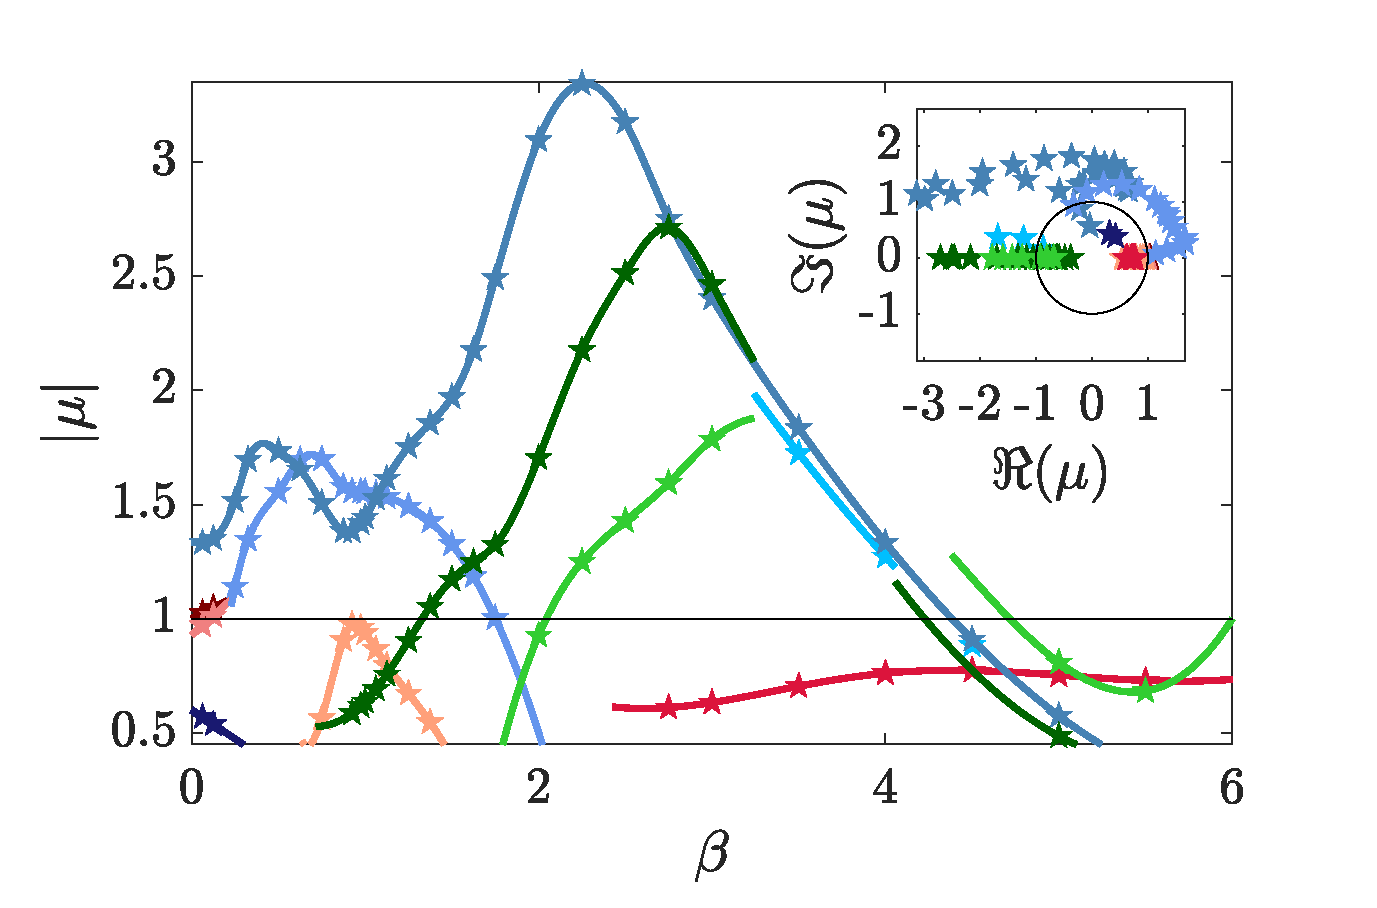
\includegraphics[width=0.49\textwidth]{./fig/AR1p25/mu_beta_Re250.eps}
  \caption{Modulus of the Floquet multipliers for $\AR=1.25$ at different $Re$. In order, the panels are for $Re=210$, $Re=220$, $Re=230$, $Re=240$ and $Re=250$.}
  \label{fig:mult-AR1p25}
\end{figure}
%
Figure \ref{fig:mult-AR1p25} shows the dependence of the Floquet multipliers on Reynolds number for the intermediate aspect ratio $\AR=1.25$, which corresponds to the case where the base flow exhibits the strongest sensitivity to $Re$. The multipliers $\mu_A$ and $\mu_B$ display a non-monotonic dependence on $Re$: both modes $A$ and $B$ are destabilised as $Re$ increases up to approximately $200$, but subsequently restabilise at higher Reynolds numbers. In particular, mode $B$ is stable at $Re \gtrapprox 240$.

For this intermediate $\AR$, additional multipliers cross the unit circle as the Reynolds number increases beyond $Re \gtrapprox 230$. At $Re \approx 230$, a pair of complex-conjugate multipliers with negative real parts and non-zero imaginary parts cross the unit circle, indicating the onset of a new quasi-periodic instability---labelled as mode $QP'$ in figure \ref{fig:modes}(e). Further increasing the Reynolds number to $Re \approx 240$, we observe the emergence of another instability: a real Floquet multiplier with positive real part crosses the unit circle. This mode is synchronous and shares the same symmetry as modes $B$ and $B'$, but has a significantly shorter wavelength, corresponding to $\beta \approx 0.5$, see mode $B''$ in figure \ref{fig:modes}(f). Since these represent higher-order bifurcations of the base flow, their detailed characterisation lies beyond the scope of the present work.


\textcolor{blue}{
For $\AR=2$ we observe that at low $Re$ only mode $A$ becomes unstable. Then, similarly to what observed for smaller $\AR$s, this mode stabilises at larger $Re$. For these $Re$ the flow is again two-dimensional. This is further confirmed by the non linear simulations. The flow then becomes again unstable to three-dimensional perturbations at larger $Re$.
}
\begin{figure}
  \centering
  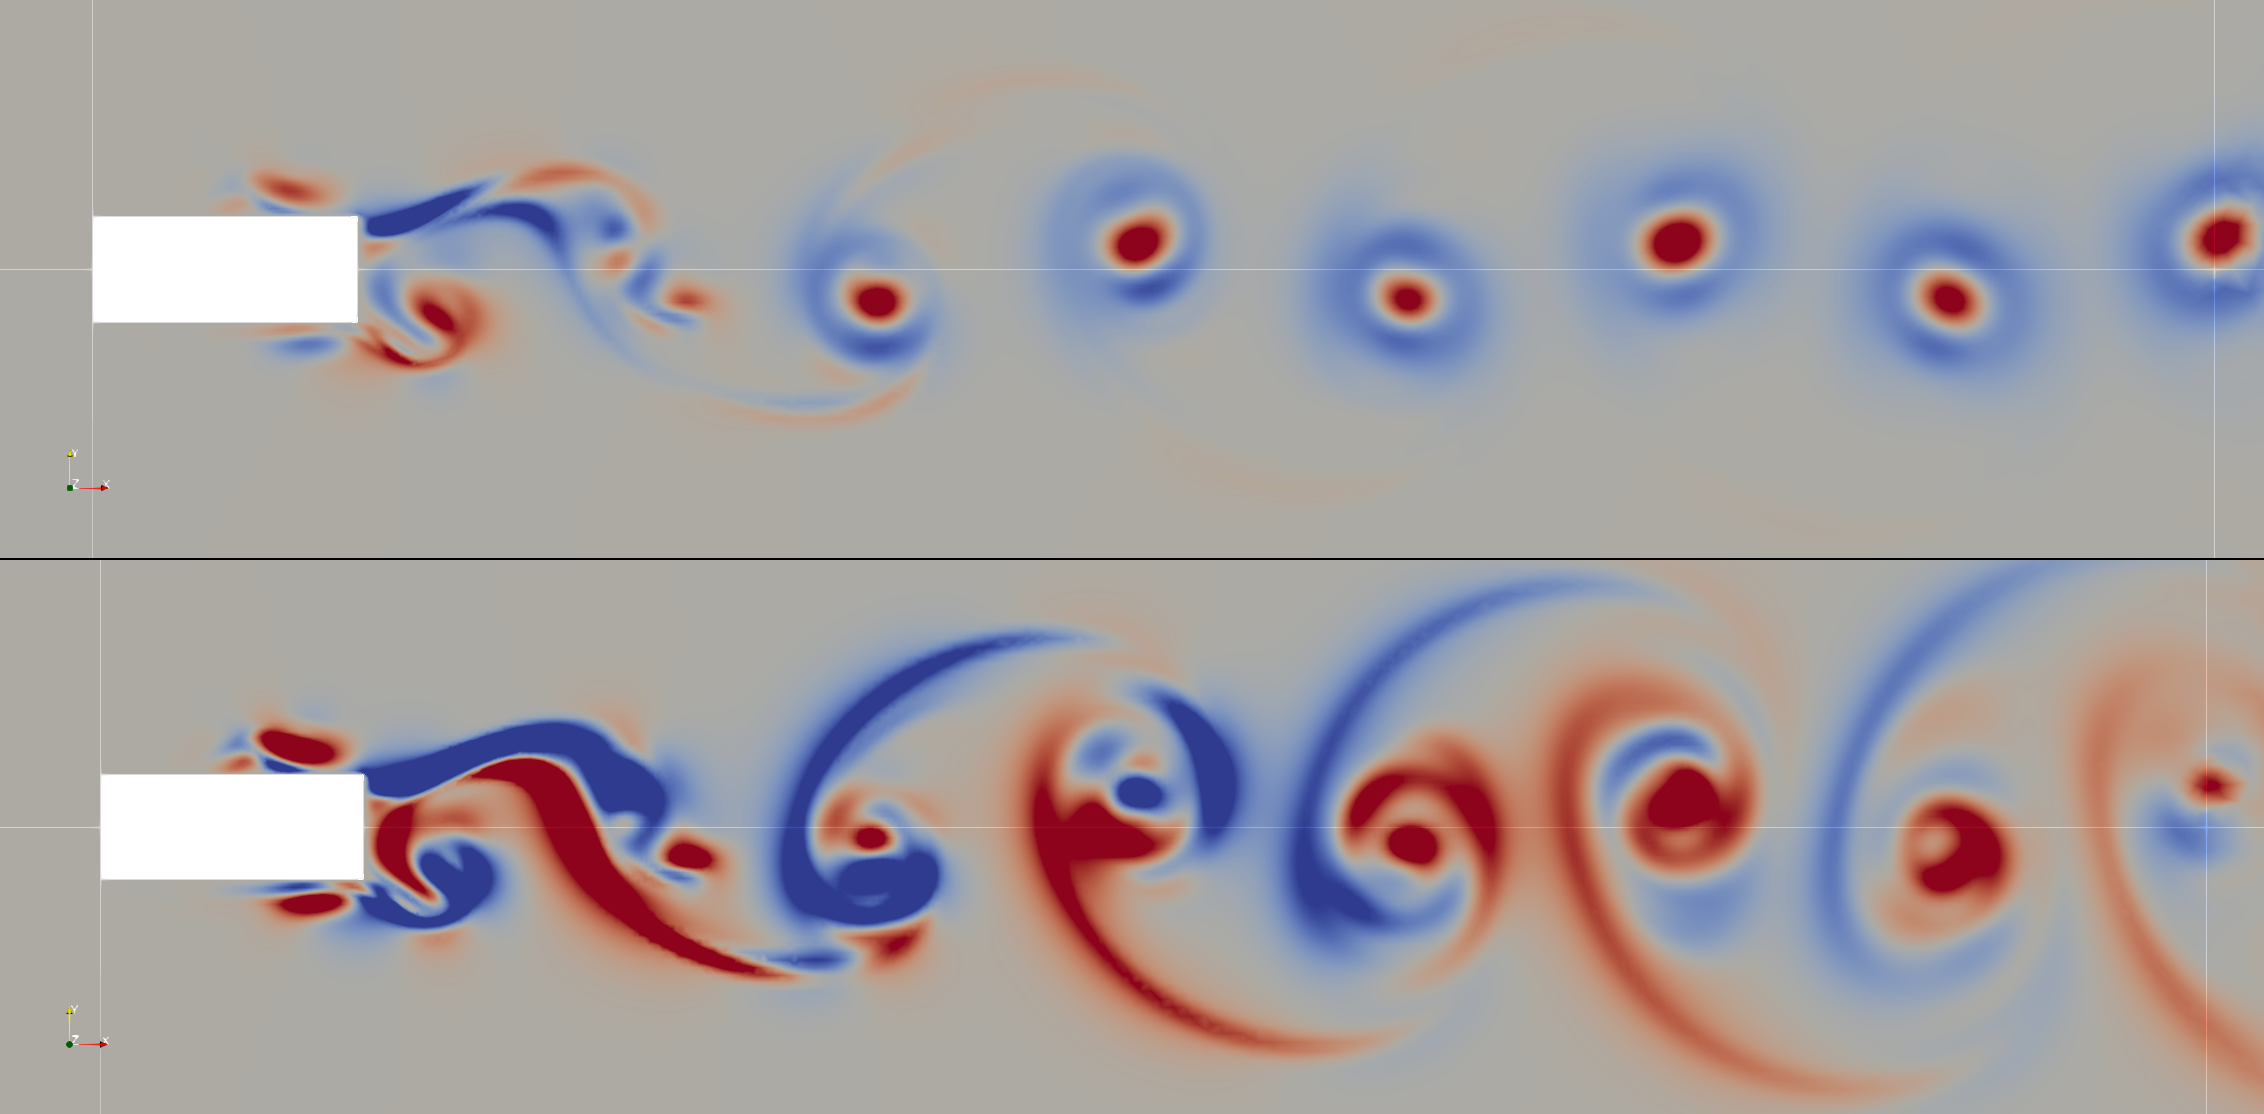
\includegraphics[width=0.32\textwidth]{./fig/AR2p5/u_Re625_beta4.png}
  \includegraphics[width=0.32\textwidth]{./fig/AR2p5/v_Re625_beta4.png}
  \includegraphics[width=0.32\textwidth]{./fig/AR2p5/w_Re625_beta4.png} 
  \caption{Unstable modes for $\AR=2.5$, $Re=625$ and $\beta=4$. From left to right the panels are for $\Re(\hat{u})$, $\Re(\hat{v})$ and $\Im(\hat{w})$. Top panels are for the most unstable mode, the bottom panels are for the less unstable one.}
  \label{fig:AR2p5modes}   
\end{figure}
\textcolor{blue}{
For $\AR=2.5$ the scenario is slightly different. In this case, indeed, the Floquet modes associated with mode $A$ approach the unit circle in the complex plane, but they do not cross it. This means that for all $Re$s the real multiplier $\mu$ associated with this mode has modulus always smaller than $1$. For this $\AR$ the flow becomes three-dimensional only at larger $Re$. The Floquet stability analysis predicts that two real multipliers cross the unit circle in short succession for $600 \le Re \le 625$. These multipliers are associated with synchronous modes.
The most unstable mode is shown in figure \ref{fig:AR2p5modes} and has the following symmetries
\begin{equation}
  \begin{aligned}
    u(x,y,t) = &+ u(x,-y,t+T/2) \\
    v(x,y,t) = &- v(x,-y,t+T/2) \\
    w(x,y,t) = &+ w(x,-y,t+T/2) 
  \end{aligned}
\end{equation}
}

\textcolor{blue}{
The second unstable mode is instead shown in figure \ref{fig:AR2p5modes} and has the following symmetries
\begin{equation}
  \begin{aligned}
    u(x,y,t) = & -u(x,-y,t+T/2) \\
    v(x,y,t) = & +v(x,-y,t+T/2) \\
    w(x,y,t) = & -w(x,-y,t+T/2)
  \end{aligned}
\end{equation}
}

\textcolor{blue}{
Unlike the unstable modes detected for smaller $\AR$s, here we observe that these modes extend also along the lateral sides of the body, suggesting that in somehow the dynamics of the LE vortices plays a certain role.}

\textcolor{red}{We have to verify whether the same two modes becomes unstable for $\AR=2$. Then, for these modes it would be interesting to look at the structural sensitivity}

\subsection{Non linear simulations}

XX 3D Simulations for $\AR=1.25, 2, 2.5$ at different $Re$. Show the phase space plots and spectra to characterise the competition between the modes. If needed we can do POD to separate the modes XX

\begin{figure}
  \centering
  \includegraphics[width=0.24\textwidth]{./fig/nnl/ClCdAR1.5RE190.png}
  \includegraphics[width=0.24\textwidth]{./fig/nnl/ClCdAR1.5RE200.png}  
  \includegraphics[width=0.24\textwidth]{./fig/nnl/ClCdAR1.5RE210.png}
  \includegraphics[width=0.24\textwidth]{./fig/nnl/ClCdAR1.5RE230.png}
  \includegraphics[width=0.24\textwidth]{./fig/nnl/ClCdAR1.5RE250.png}
  %\includegraphics[width=0.49\textwidth]{./fig/AR1p25/mu_beta_Re250.eps}
  \caption{Cl vs Cd for $\AR=1.5$ at different $Re$.}
  \label{fig:ClCd}
\end{figure}

\begin{figure}
  \centering
  \includegraphics[width=0.24\textwidth]{./fig/nnl/psdAR1.5RE190.png}
  \includegraphics[width=0.24\textwidth]{./fig/nnl/psdAR1.5RE200.png}  
  \includegraphics[width=0.24\textwidth]{./fig/nnl/psdAR1.5RE210.png}
  \includegraphics[width=0.24\textwidth]{./fig/nnl/psdAR1.5RE230.png}
  \includegraphics[width=0.24\textwidth]{./fig/nnl/psdAR1.5RE250.png}  
  %\includegraphics[width=0.49\textwidth]{./fig/AR1p25/mu_beta_Re250.eps}
  \caption{Psd for $\AR=1.5$ at different $Re$.}
  \label{fig:ClCd}
\end{figure}

This section describes 3-D wake transition process and mode interactions at different Reynolds number and for different aspect ratios. To this aim, we performed direct numerical simulation XXX DettaigliXXX. The initial condition has a slight effect in determining the exact onset for the instability of modes \cite{jiang-cheng-an-2018}. In this specific case, we started from a 2D solution obtained with a potential solution of the flow, and we initially triggered a disturb of the type XXX. 




Our study started from the smaller aspect ration, $\AR=1.5$. From the Floquet instability analysis of \S \ref{sec:short}, at $Re=200$ the flow becomes unstable due to mode A. For this reason, we performed simulations from $Re=170$ to $Re=250$, with a gap of $\Delta Re=20$.XXX COMPLETE ONCE \S \ref{sec:short} HAS MORE DETAILS AND WE ARE SUREXXX. For each dataset, we computed the streamwise vorticity $\omega_x$ which has been used to characterize the wake. The two dimensional von Kármán wake persist until $Re=210$. From $Re \leq 210$ the wake undergoes a secondary instability leading to a three-dimensional state.

\begin{figure}
  \centering
  \includegraphics[trim={12cm 0 12cm 0},clip,width=0.49\textwidth]{./fig/Wake/AR1.5Re200.png}     
  \includegraphics[trim={12cm 0 12cm 0},clip,width=0.49\textwidth]{./fig/Wake/AR1.5Re210.png}   
  \includegraphics[trim={12cm 0 12cm 0},clip,width=0.49\textwidth]{./fig/Wake/AR1.5Re230.png} 
  \includegraphics[trim={12cm 0 12cm 0},clip,width=0.49\textwidth]{./fig/Wake/AR1.5Re250.png}
  \caption{Isocontours of $\omega_x$ of the three dimensinal wake for $Re=200$ (top-left panel), $Re=210$ (top-right panel), $Re=230$  (bottom-left panel), $Re=250$ (bottom-right panel).}
  \label{fig:wake1.5}
\end{figure}  

 Figure \ref{fig:wake1.5} shows instantaneous $\omega_x=XXX$ isocontours for $Re=210$, $Re=230$, and $Re=250$. At the lowest Reynolds number, the instability is due to mode A.


%\section{A far wake instability for intermediate $\AR$s}

For the circular cylinder case it is well known \citep{vorobieff-goergiev-ingber-2002,kumar-mittal-2012} that the primary vortex street in the near wake transitions into a two-layered vortex street in the intermediate wake, followed by a transition from the two-layered vortices to a secondary vortex steet in the far wake.

The physical mechanism for the first transition was investigated by \cite{durgin-karlsson-1971}, \cite{karasudani-funakoshi-1994} and \cite{dynnikova-guverntuk-2016}. According to their results the breakdown of the primary vortex street is the result of the convection of vorticity within a vortex by the other vortices of the street. The physical mechanism for the second transtion has been attributed to the hydrodynamic instability of the mean wake flow \citep{cimbala-nagib-roshko-1988,williamson-prasad-1993}, and to the convective instability of the mean wake flow \citep{kumar-mittal-2012}.

The streamwise location for the second transition has been largely examined over the last years. For example \cite{inoue-yamazaki-1999} and  \cite{vorobieff-etal-2002} by means of two-dimensional numerical simulations and soap-film experiments increased the Reynolds number uo to $Re=1000$. They observed that the streamwise location of the second transition moved upstream with increasing $Re$, with a proposed law for the transition location of $\sim Re^{-1/2}$. 

More recently, \cite{jiang-cheng-2019} provided a detailed investigation of the far wake instabilities of the flow past a circular cylinder using two-dimensional simulations. They observed that the transition to the secondary vortex street is driven by two different processes depending on the Reynolds number. For small $R$, the transition process is dictated by the merging of two same-sign vortices, while at larger $Re$ it is driven by the pairing of two opposite-sign vortices followed by the merging of the paired vortices.


\cite{thompson-etal-2014} consdiered the flow past two-dimensional elliptic cylinders with the major axis placed normal to the flow direction, ranginf from a circular cylinder to a flat plate placed perpendicular to the incoming flow. They investigated the developement of the secondary vortex street for different geometries. At $Re=100$, tor the cyrcular cylinder they observed that the near wake is the classical K\'{a}rm\'{a}n vortex street, that further downstream develops into a two-layered wake. Moving downstream, they observed that the clockwise and anticlockwise vortices diffuse and crossannihilate, leaving a featureless wake. Increasing $Re$ the same scenario is observed, with the two-layered wake arising more downstream. When decreasing $\AR$, instead, the observed that the transition process is accelerated. For example, for $\AR=0.5$ at $Re=200$ they observed that the transition from the K\'{a}rm\'{a} street to the two-layered street occurs within two diameters past the cylinder and that the stationary wake does not form at all. \textcolor{red}{Interestingly, they observed that for small $\AR$ as $Re$ increases the transition migrates upstreams and the developement of the mode A instability is suppressed. This shows that at smaller Reynolds number the near-wake is threedimensional. But then, increasing $Re$ the transition of the two-dimensional wake moves upstream and suppressed the global instability. A simila scenario with modes that become unstable and then stabilise again as $Re$ increases has been observed for the flow past rotating cyilinder \citep{rao-etal-2013,radi-etal-2013}. XX This is similar to what we do observe for $\AR=2.5$ apparently. Look at the base flow to further understand what happens. XX}


\cite{durgin-karlsson-1971} considered a von K\'{a}rma\'{a}n vortex street subjected to a deceleration. This modifies the ratio of longitudinal to lateral spacing between the vortices. They observed that the distortion of the individual vortices resultes in annihilation of concentrated vortex regions and creation of a stationary wake flow. This resulting wake flow is itself dynamically unstable and develops into a new vortex street of a different frequency form the initial one. They explained the breakdown of the initial vortex street with the convection of a concentrated vortex region due to the motion imposed by all the other vortices. In 1959 Taneda discovered that far downstream the original vortex street disappears and a new one of larger scales appears. His results were later confirmed by the observation of \cite{zdravkovich-1968} who photographed the vortex trails of three cylinders in close proximity. They considered this problem experimentaly, by looking at the vortex street generated from a cyrcular cylinder ad develerated by the presence of a downstream larger circular cylinder placed perpendicular to the first one and to the flow. Between the two cylinder they observed that the K\'{a}rm\'{a}n vortex street changes structure. More specifically, near the outside of the wake the measure a single frequency sinusouidal wake. \textcolor{red}{When the probe was moved closer to the centreline, they observed that a dominat second harmonic component arises. This is well documented i Kovasznay (1949) and Roshko (1953)}. When moving downstream they observed that the fluctuations become smaller and finally become not detectable. This corresponds to the two-layer region and is referred to as the calm region. Here no velocity fluctuations are visible in the centreline. The end of this calm region is detected by the development of a grwoing instability and the formation of a new vortex street with much larger widft and wavelength than the original. \textcolor{red}{They observed that the frequency of the primary and secondary wake exhibit a linear relation, see their figure 3}. A good way to recognise the primary vortex street, the calm region and the secondary vortex street is to look at the mean velocity at the centreline. Here $U$ exhibits a clear drop in the calm region, before recovering in the secondary vortex street. \textcolor{red}{What if we simply look at instantaneous snapshots? The problem is that the regions where the two vortex street are generated may change in time, so we do not have in this way a statistical information of the ``average'' points}. They measure the longitudinal shape of the vortex filaments by using correlations. In particular they detected the position of the vortex positions by looking at the zero correlation points. They observed that the vlaues of the downstream spacing $a$ between two shed vortices decreases by approximately $60\%$ along tha primary vortex street. \textcolor{blue}{How do we measure this? We can simply look at the local maxima of the vorticity for example. However, some references for example Hooker (1936) mentioned that this points is not exacly the same as the point where the fluid appears to rotate because of the vorticity diffusion}. This considerably devates form that of a vortex street in uniform flow which exhibits a realstively constant value in downstream spacing \citep{schaefer-eskinazi-1959}. They propose a model using a Hamel--Oseen vortex model for the vortices and observed that the arise of the calm region is related to the moment where $h/a<0.366$. In this case the part of the vortex outside the vortex street leads the inside part in the downstream direction. Therefore, these vortices starts deforming due to their mutual interaction and then, after deformed, they annihilate each other giving rise to the so-called calm region. They report that the calm regions consists (on average) of two adjactent layers of vorticity of opposite sigs. Here the mean velocity profiles are reminescent of the laminar wake formed behind a flat plate in a uniform stream. These shear layers are then unstable and give rise to the secondary vortex street. The scenario described by \cite{durgin-karlsson-1971} was later confirmed by the experimental work of \cite{karasudani-funakoshi-1994}.

\cite{taneda-1959} suggested that the origin of the secondary vortex street of large scale may be explained by the linear stability theory for the locoal mean wake profile, which changes slowly in the streamwise direction. Matsui and Okude (1982) and Okude and Matsui (1990) proposed that the secondary vortex street is formed by the pairing of the vortices in the primary vortex steet. That is, they claimed that the wavelength of the vortex street becomes larger as a result of the pairing of vortex regions, withoug actually going through a parallel shear flow state. However, successive results presented for example by \cite{karasudani-funakoshi-1994}. Indeed, by looking at the wavelengths of the primary and secondary vortex streets, i.e. $a_1$ and $a_2$ they do not observe that the ratio $a_2/a_1$ is close to $2$ for a wide range of $Re$, as expected in the case of vortex pairing. Similarly, the ratio of the frequencies $f_1/f_2$ is observed for decrease with increasing $Re$, again in contraddiction with the vortex pairing scenario where instead $f_1/f_2$ should be close to 2. 

\textcolor{red}{XX PLOT A ZOOM OF THE DIFFERENT FLOW REGIONS, TO SHOW THAT THE PRIMARY VORTEX STREET EVOLVES INTO A NEARLY PARALLEL SHEAR FLOW, BEFORE THE SECONDARY VORTEX STREET ARISES xx}

\textcolor{blue}{XX Can we detect the centre of the vortices to measure $h$ and $a$ using the local maxima of the vorticity?  I have to compute $h_1$ and $h_2$, i.e. the transverse spacing of neighbouring vortex regions of opposite signs in the primary and secondary wakes and $a_1$ and $a_2$, i.e. the longitudinal spacing of vortex regions of the same sign in the parimary and secondary vortex streets respectively XX} 

\cite{karasudani-funakoshi-1994} observed that since a nearly parallel flow is observed before the secondary vortex street, it is reasonable to predict that the formation of this vortex street is the result of the instability of the parallel flow, similarly to what predicted by \cite{taneda-1959} and \cite{cimbala-1988}. They used the data of \cite{fujimura-etal-1988} that calculated the linear stability of the parallel flow, approximating the velocity profiles with Gaussian cruves.

\cite{jhonson-thompson-hourigan-2004}

\cite{alksyuk-shkadova-shkadov-2012}

Apart from viscous diffusion, the geometric arrangement of the vortices in the vortex street determines whether is it predominately stable or whether it breaks fown into a parallel shear flow. \cite{durgin-karlsson-1971} defined a critical value of $h/a = 0.365$ where $h$ is the cross-wake spacing between positive and negative wake vortices, while $a$ is the separation between vortices of the same sign. Above this critical value, the vortices stretch our and aling with the downstreamw direction leading to a parallel shear flow. In turn, this mean shear flow can become unstable forming a secondary vortex street. This process was further investigated by \cite{karasudani-funakoshi-1994}.

Although the scope of the present work is not on this we report some results.

\begin{figure}
  %\includegraphics[trim={0 1060 0 0},clip,width=\textwidth]{./fig/appendix/AR2p5_Re450.png}
  %\includegraphics[trim={0 1060 0 0},clip,width=\textwidth]{./fig/appendix/AR2p75_Re450.png}
  %\includegraphics[trim={0 1060 0 0},clip,width=\textwidth]{./fig/appendix/AR3_Re450.png}
  %\vspace{0.5cm}
  %\includegraphics[trim={0 1060 0 0},clip,width=\textwidth]{./fig/appendix/AR3p5_Re450.png}
  %\includegraphics[trim={0 1060 0 0},clip,width=\textwidth]{./fig/appendix/AR5p5_Re450.png}
  %\includegraphics[trim={0 1060 0 0},clip,width=\textwidth]{./fig/appendix/AR6_Re450.png}    
  \includegraphics[width=\textwidth]{./fig/appendix/AR_2_2p75_Re450.png}
  \includegraphics[width=\textwidth]{./fig/appendix/AR_3_4_Re450.png}
  \includegraphics[width=\textwidth]{./fig/appendix/AR_5p5_6p25_Re450.png}    
  \caption{Instantaneous visualisations of the far wake at $Re=450$ for $\AR=2,2.25,2.5,2.75$ (top), $\AR= 3, 3.25, 3.5, 4$ (centre) and $\AR=5.5,5.75,6,6.25$ (bottom). The transition to the two-layered vortex steet and the sucessive transition to the secondary vortex street occurs at different streamwise positions depending of $\AR$. It seems that the transition moves upstream as $\AR$ is increased towards the end of the oblique brach, i.e. towards the point where the TE vortex shedding is permitted. In the case where the flow dynamics is governed by the LE vortex shedding we have that the transition is instead moved downstream. The vortex interaction in the primary vortex street is such that the transition is delayed. We have to verify the $h/a$ threshold to compared with the theory. XX CHECK THE FREQUENCY AT THE DIFFERENT STATIONS. ADD ALSO OTHER $\AR$s. \textcolor{red}{DO WE WANT THE AVERAGE FIELD, WITHOUT WE CAN NOT DO SEVERAL THINGS} XX}
  \label{fig:wake}
\end{figure}

\begin{figure}
\centering
\includegraphics[width=0.328\textwidth]{./fig/appendix/uv_xw_AR3_Re450_a.eps}
\includegraphics[width=0.328\textwidth]{./fig/appendix/uv_xw_AR3_Re450_b.eps}
\includegraphics[width=0.328\textwidth]{./fig/appendix/uv_xw_AR3_Re450_c.eps}
\includegraphics[width=0.328\textwidth]{./fig/appendix/Spec_AR3_Re450_a.eps}
\includegraphics[width=0.328\textwidth]{./fig/appendix/Spec_AR3_Re450_b.eps}
\includegraphics[width=0.328\textwidth]{./fig/appendix/Spec_AR3_Re450_c.eps}
\caption{Phase space diagrams and frequency spectra plots in the wake for $\AR=3$ and $Re=450$. Top: $u-v$ diagrams at different streamwise locations. Bottom: frequency spectra $S(v)$ at different streamwise locations. Left: primary vortex street. Centre: two-layered wake. Right: secondary vortex street.}
\label{fig:wake_AR3}
\end{figure}

\begin{figure}
\centering
\includegraphics[width=0.328\textwidth]{./fig/appendix/uv_xw_AR6_Re450_a.eps}
\includegraphics[width=0.328\textwidth]{./fig/appendix/uv_xw_AR6_Re450_b.eps}
\includegraphics[width=0.328\textwidth]{./fig/appendix/uv_xw_AR6_Re450_c.eps}
\includegraphics[width=0.328\textwidth]{./fig/appendix/Spec_AR6_Re450_a.eps}
\includegraphics[width=0.328\textwidth]{./fig/appendix/Spec_AR6_Re450_b.eps}
\includegraphics[width=0.328\textwidth]{./fig/appendix/Spec_AR6_Re450_c.eps}
\caption{As figure \ref{fig:wake_AR6}, but for $\AR=6$. XX UPDATE WITH MORE DATA XX.}
\label{fig:wake_AR6}
\end{figure}

We start considering $\AR=3$ at $Re=450$ as an example, see figure \ref{}. The wake flow can be separated into three regimes, namely the primary vortex street, the two layered vortices and the secondary vortex street. Following \cite{jiang-cheng-2019} the streamwise locations of the first and second transitions can be determined by the time-averaged $\langle v \rangle$ field. Indeed, two pairs of local maxima are observed in correspondence of this transition, as here the flow is diverted away from the wake centreline. The second location of local maxima of $\langle v \rangle$, instead, corresponds to the second transition where the flow starts to reoccupy the wake centreline. The distinction between the different flow regimes is evident also when looking at the time-averaged Reynolds shear stresses $\langle u'v' \rangle$. Accordingly, the Reynolds shear stresses are substantially null in the two-layered region, which is commonly referred to as the ``calm region'' \citep{durgin-karlsson-1971}.

We now show the influence of $\AR$. Here the focus in of $\AR \ge 2.5$ and fix the Reynolds number to $Re=450$. Results for $4 \le \AR 4.5$ are not reproted, as here at this $Re$ the near wake undergoes a two-dimensional instability which leads to a slanted wake. In this case the two-layered wake and the secondary vortex street are not observed. \textcolor{red}{XX Dependence of the position of the two transitions points on $\AR$ at this $Re$, explain how this changes with the near-wake flow topology XX}

Figure \ref{} shows the frequency spectra of the time histories of $v$ sampled at $y=0$ and various $x$ positions for different $\AR$s. \textcolor{red}{XX Figure with different pannels. For each panel we show the frequency spectra at different $x$ positions for different $\AR$s XX}We look at the spectra of $u_y$. Accordinlgly, two peaks $f_1$ and $f_2$ are observed in the spectra. The first is well defined and represents the primary vortex shedding frequency. The second peak, instead, consist of a sharp peak together with small-scale broad-band frequencies and is associated with the development of the secondary vortex street. This is clearly shown in figure \ref{}, where the $v$ time signal is shown at two different streamise locations dominated by primary and secondary vortex street. \textcolor{red}{XX Add (i) dependence of $f_1$ and $f_2$ on $x$ and $\AR$, (ii) dependence on $x$ of the intensity of the two peaks for different $\AR$s}.

\textcolor{red}{Do we plot also the evolution of the wake deficit for the different cases? $(1-\langle u \rangle/U_\infty)$}

\cite{durgin-karlsson-1971}, \cite{tsuboi-oshima-1985} and \cite{karasudani-funakoshi-1994} investigated the stability of the geoemtrical arrangement of vortices in a wake shown that when the spacing ratio $h/a$ was larger that $0.365$, the vortices would rotate to align with the streamwise direction and stretch out and diffuse resulting into a near-parallel shear flow. When this flors, the near-stationaly wake is convectively unstable and may form a new secondary vortex street with a longer wavelenght and a lower frequency. This has been investigated also by \cite{thompson-etal-2014} in the context of the flow past two-dimensional elliptic bluff bodies. Figure \ref{} shows the variation of the spacing ration with downstream distance for a number of different $\AR$s. \textcolor{red}{XX Comment on what we observed and the streamwise location at which we observe that the ratio becomes larger than the threshold. Relate this with the above discussion XX}


\textcolor{red}{We can perfrom DMD analysis of the far wake. Look at \cite{thompson-etal-2014}.}


\iffalse

\begin{figure}
  \centering
  \includegraphics[width=0.8\textwidth]{./fig/AR3/BF_vort_Re400_475.png}
  \includegraphics[width=0.5\textwidth]{./fig/AR3/T_Re.eps}
  \caption{Base flow vorticity snapshots for $\AR=3$ at (from top to bottom) $Re=400$, $Re=425$, $Re=450$ and $Re=485$. Note that as $Re$ increases the structure of the wake changes, with the positive and negative vorticity monopoles being clearly separated. As $Re$ increases, this separation start occurring closer to the TE. Bottom panel: Dependence of the period $T$ on $Re$ for the periodic regime in the $350 \le Re \le 485$ range.}
  \label{fig:BF_AR3}
\end{figure}

\begin{figure}
  \centering
  \includegraphics[width=0.5\textwidth]{./fig/AR3/mult_Re495_beta0.eps}
  \includegraphics[width=1.0\textwidth]{./fig/AR3/Floquet_modes_beta_0_Re495.png}
  \caption{Floquet analysis for $\AR=3$ and $Re=495$. Top: Floquet multilpiers for $\beta = 0$. Bottom: Modes associated with the $4$ multipliers outside the unit circumference.}
  \label{fig:AR3_Stab}
\end{figure}

\begin{itemize}
  \item For $\AR=3$ we observe that the wake becomes unstable in the far wake.
  \item Study Batchelor and Lamb. Look for instability of trains of vortices
  \item How can the far wake be influenced by the body? Porbaby we have this phenopmena also at different AR, and with different bodies, but it happens at conditions different from the one we observed, since the wake is already 3d, or, for example at AR=4, the wake become storta so we do not see this phenomenom.
\end{itemize}

\fi

\section{Intermediate $\AR$s with $3 < \AR < 4.75$}
\label{sec:int}

We now focus on the horizontal $n=1$ branch, dominated by LE vortex shedding (see figure~\ref{fig:StLAR}), corresponding to the aspect ratio range $3 \leq \AR \leq 4.75$. Within this regime, we select $\AR=4$ and $\AR=4.5$ as representative cases. For these aspect ratios, the secondary bifurcation is triggered by a two-dimensional instability that leads to a deviated wake. To the best of our knowledge, this phenomenon has not been previously reported for symmetric two-dimensional bluff bodies.

\subsection{A $2D$ bifurcation}

\subsubsection{Non linear simulations}


\begin{figure}
  \centering
  \includegraphics[trim={0 100 0 100},clip,width=0.49\textwidth]{./fig/vort_Re425_25.png}
  \includegraphics[trim={0 100 0 100},clip,width=0.49\textwidth]{./fig/vort_Re450_25.png}  
  \includegraphics[trim={0 100 0 100},clip,width=0.49\textwidth]{./fig/AR4p5/vort_Re430_25.png}
  \includegraphics[trim={0 100 0 100},clip,width=0.49\textwidth]{./fig/AR4p5/vort_Re450_25.png}
  \caption{Instantaneous snapshots for $\AR=4$ at $Re=425$ (top left) and $Re=450$ (top right), and $\AR=4.5$ at $Re=430$ (bottom left) at $Re=450$ (bottom right).}
  \label{fig:snap_ar4_ar4p5}
\end{figure}

Nonlinear simulations reveal that as the Reynolds number increases to the critical value $Re = Re_{c2}$, the 2D periodic base flow becomes unstable to 2D perturbations, undergoing a synchronous bifurcation. The resulting flow maintains the original temporal periodicity but develops a distinct slanted wake. This transition is illustrated in figure \ref{fig:snap_ar4_ar4p5}, which shows instantaneous vorticity fields at various Reynolds numbers.

For $Re \le Re_{c2}$ (left panels), the wake remains aligned with the $x$-axis and exhibits the canonical von-K\'{a}rm\'{a}n-like vortex shedding pattern, characterised by alternating vortices of opposite sign shed along the centerline $y=0$. This flow regime, extensively analysed in \cite{chiarini-quadrio-auteri-2022}, is briefly recalled here for completeness. In this parameter range, the dynamics are dominated by leading-edge (LE) vortex shedding, where a single vortex alternately forms on each side of the cylinder. These LE vortices convect downstream and, upon traversing the trailing edge (TE), induce a hyperbolic stagnation point that triggers the subsequent shedding of a TE vortex of opposite sign from the opposing side \citep{chiarini-quadrio-auteri-2022}.
%
Critically, the timing of the LE vortex passing the TE corner is phase-locked with the shedding of the associated TE vortex. The relative phase shift between LE passage and TE shedding exhibits a mild dependence on the aspect ratio, accounting for observed variations in wake topology between the $\AR=4$ and $\AR=4.5$ configurations. Specifically, the LE vortices downstream are markedly attenuated for $\AR=4$ compared to $\AR=4.5$.

Beyond the critical Reynolds number $Re_{c2}$, the flow undergoes a bifurcation characterised by the loss of reflectional symmetry about the centerline $y=0$, leading to a persistent wake deviation. In this regime, the vortex monopoles no longer remain aligned along $y=0$, but are displaced either above or below the centerline. For $\AR=4$, this symmetry-breaking transition occurs at $Re \ge Re_{c2} \approx 435$, wherease for $\AR=4.5$, it manifests at a slightly lower threshold $Re \ge Re_{c2} \approx 417.5$. The direction of wake deflection---upward or downward---is determined by the initial flow conditions and is effectively random.

\begin{figure}
  \centering
  \includegraphics[width=0.49\textwidth]{./fig/AR4_Cl_Re.eps}
  \includegraphics[width=0.49\textwidth]{./fig/AR4_Cd_Re.eps}
  \includegraphics[width=0.49\textwidth]{./fig/AR4_T_Re.eps}
  \caption{Dependence of $C_\ell$, $C_d$ and $T$ on the Reynolds number $Re$. The straight wake for $Re>Re_{c2}$ has been stabilised by means of the BoostConv algorithm.}
  \label{fig:Cl-Cd-AR4}
\end{figure}
%
To further characterise this bifurcation, figure \ref{fig:Cl-Cd-AR4} presents the Reynolds number dependence of the aerodynamic force coefficients---lift $C_\ell$ and drag $C_d$---as well as the flow period $T$ for $\AR=4$. For $Re>Re_{c2}$, the unstable straight-wake solution is stabilised via the BoostConv algorithm. Consistent with flow symmetry, the time-average lift coefficient remains zero $\langle C_\ell \rangle = 0$ for $Re \le Re_{c2}$, while it departs from zero $\langle C_\ell \rangle \neq 0$ for $Re>Re_{c2}$, indicating the symmetry-breaking associated with the bifurcation. In contrast, the drag coefficient exhibits a monotonic increase with Reynolds number across both regimes, with a notably steeper slope in the deviated wake state. Figure \ref{fig:Cl-Cd-AR4}(c) further substantiates the synchronous nature of the bifurcation: the flow period $T$ for both the symmetric and deviated wake solutions collapses onto a single curve, decreasing smoothly with increasing $Re$. The continuous, smooth behaviour of the $C_\ell-Re$ and $C_d-Re$ curves strongly suggests a supercritical or smooth bifurcation. This characterisation will be explored in greater detail in subsequent sections.

\subsubsection{Linear stability analysis}
\begin{figure}
\centering
\includegraphics[width=0.49\textwidth]{./fig/AR4p5/multipliers_2D.eps}
\includegraphics[width=0.49\textwidth]{./fig/AR4p5/multipliers_2D_b.eps}
\includegraphics[width=0.7\textwidth]{./fig/AR4p5/omegaz_beta0_Re430_AB.png}
\includegraphics[width=0.7\textwidth]{./fig/AR4p5/Floqetmode_beta_0_Re450_AR4p5.png}
\caption{$2D$ bifurcation of the periodic flow past a rectangular cylinder with $\AR=4.5$. Top: Multipliers associated with the straight (solid) and slanted (dashed) wake for $\AR=4.5$. The left panel plots $|\mu|$ as a function of $\beta$. The red colour refers to real and positive multipliers, while the blue colour refer to complex mutlpliers. The right panel shows the dependence of $\Re(\mu)$ and $\Im(\mu)$ on $Re$. Note that the slanted wake is the results of the synchronous instability described by the red branch. Once the wake becomes slanted a new branch with complex conjugate multipliers arises that becomes unstable at $Re \approx 450$. Centre: Floquet modes associated with the straight wake; the colours are for the spanwise vorticity and the above and bottom panel refer to the red and blue branches respectively. Bottom: Floquet mode associated with the blue branch of the slanted wake.}
\label{fig:AR4p5_modes_Re430_beta0}
\end{figure}

To elucidate the origin of the slanted-wake phenomenon, we conduct a linear stability analysis of the straight wake against 2D ($\beta=0$) perturbations employing Floquet theory. Although both aspect ratios $\AR=4$ and $\AR=4.5$ are examined, we present results exclusively for $\AR=4.5$ for conciseness.

Figure \ref{fig:AR4p5_modes_Re430_beta0}(a--b) displays the Floquet multipliers computed for the straight-wake base flow. Synchronous modes, characterised by real and positive multipliers, are highlighted in red, whereas complex-conjugate pairs representing quasi-periodic modes are shown in blue.
%
The red branch crosses the unit circle at $Re=Re_{c2} \approx 417.5$ for $\AR=4.5$; a similar crossing occurs near $Re_{c2} \approx 425$ for $\AR=4$. The zero imaginary part of the critical multiplier $\Im(\mu) = 0$ at onset confirms the synchronous nature of the bifurcation, indicating that the slanted wake emerges via a global instability of the straight-wake base flow. Meanwhile, the quasi-periodic branch (blue) remains stable within the investigated Reynolds number range.

Further insight is provided in figure~\ref{fig:AR4p5_modes_Re430_beta0}(c), which depicts the spanwise vorticity field of the unstable Floquet mode overlaid on isolines of the base-flow vorticity. Notably, this unstable mode breaks the spatio-temporal symmetry exhibited by the periodic base flow. Consistent with the observed time-averaged symmetry breaking, the mode satisfies
%
\begin{equation}
  \hat{u}(x,y,t) = - \hat{u}(x,-y,t+T/2) \qquad \text{and} \qquad \hat{v}(x,y,t) = \hat{v}(x,-y,t+T/2)
\end{equation}
%
which leads to
%
\begin{equation}
  \hat{\omega}_z(x,y,t) = \hat{\omega}_z(x,-y,t+T/2).
\end{equation}

In the wake region, the unstable mode generates dipolar perturbations that amplify as they are advected downstream. A pronounced phase synchronisation between the base flow and the perturbation field is evident: the dipolar structures of the Floquet mode remain phase-locked with the base-flow vortices throughout the oscillation cycle.
%
Such dipolar perturbations superimposed on monopolar base-flow vortices are commonly referred to as displacement modes \citep{brion-sipp-jacquin-2014}, as they effectively shift the vorticity centroid. This mechanism aligns well with the vortex core displacements observed for $Re > Re_{c2}$ in figure~\ref{fig:snap_ar4_ar4p5}. Specifically, for a positive base-flow vortex in the wake, the associated Floquet dipole presents positive vorticity on its lower side and negative vorticity on its upper side. The superposition of these fields reinforces the lower portion of the vortex while weakening the upper part, resulting in a net downward displacement. Conversely, negative base-flow vortices exhibit an opposite dipole orientation, producing a similar downward shift. This coherent interaction explains the systematic vertical displacement of vortex centroids characteristic of the slanted-wake regime.
%
Notably, this mechanism closely parallels the displacement modes described by \citet{jallas-marquet-fabre-2017} in pitching airfoil flows.

For completeness, we also note that the slanted-wake solution itself becomes unstable to two-dimensional quasi-periodic perturbations; however, as demonstrated below, this corresponds to a secondary bifurcation of the slanted-wake base flow. In contrast, the onset of three-dimensionality arises at lower Reynolds numbers and thus represents the primary pathway to flow complexity within this regime.

\subsubsection{Non linear effects}

\iffalse
\begin{itemize}
  \item \textcolor{blue}{ Amplitude equation non è esattamente corretta. Quel valore di A che ottengo non è esattamente la stessa amplitude che si ottiene per $\hat{\bm{u}}_1$ quando si fa WNL con un'espansione alle scale multiple. Infatti in quel caso il campo di velocità dovrebbe essere $\bm{u} = \bm{u}_0 + \epsilon A(T) \bm{u}_1 ..$ dove nei termini successivi (per esempio $\bm{u}_2$) ci sono anche correzioni al flusso base. Quindi, fai attenzione non è esattamente la stessa cosa. }
  \item \textcolor{blue}{ Possiamo fare un'espansione alle scale multiple per trovare che forma ha questa amplitude equation? Possiamo fare veramente and una WNL su questa biforcazione o non è possibile? }
  \item \textcolor{blue}{ Leggi bene anche gli articoli di Barkley \& Hendersson }
  \item Aggiungi riferimento a  Kuznetsov, pagina 121 dove si parla della forma normale per quanto riguarda la biforcazione pitchfork per un sistema dinamico discreto.
\end{itemize}
\fi

\begin{figure}
  \centering
  \includegraphics[width=0.7\textwidth]{./fig/AR4p5/Nlgrowth_Re420.eps}
  \caption{Nonlinear growth of the 2D perturbation to the wake near the secondary instability threshold for $\AR=4.5$ and $Re=420$. Top: the blue circles are the amplitude of $A_n$ evaluated from simulations of the full Navier--Stokes equations at $Re=420$. The solid line shows the prediction $A_{n+1} = \mu A_n$, while the dashed line shows the prediction $A_{n+1} = ( \mu + \alpha_1 A_n + \alpha_2 A_n^3 ) A_n$, with $\alpha_1 = -0.01114$ and $\alpha_2 = 0.000359$. The inset shows the bifurcation diagram.}
  \label{fig:ar4p5_nnl}
\end{figure}

The linear stability analysis presented in the previous section captures the onset of the instability but does not provide a description of the resulting asymmetric limit cycle. While linear theory is sufficient to determine the critical Reynolds number $Re_{c2}$, understanding the flow dynamics beyond the onset requires incorporating nonlinear effects.

Near a critical point, the wake dynamics can be approximated by a reduced-order discrete-time dynamical system, as proposed by \cite{henderson-barkley-1996} and \cite{henderson-1997}. To this end, we represent the full velocity field as
%
\begin{equation}
\bm{u}(\bm{x}, t) = U \bm{u}_0(\bm{x}, t) + A(t) \bm{u}_1(\bm{x}, t),
\end{equation}
%
where $||\bm{u}_0||=1$ and $||\bm{u}_1||=1$, $\bm{u}_0$ denotes the base flow, and $\bm{u}_1$ is the leading unstable Floquet mode with time-dependent amplitude $A(t)$. To reduce the problem to a discrete map, we sample the system at discrete times $t_n = t_0 + nT$, corresponding to successive base-flow periods. The flow field at each time step becomes
%
\begin{equation}
\bm{u}(\bm{x}, t_n) = U \bm{u}_0(\bm{x}, t_n) + A_n \bm{u}_1(\bm{x}, t_n),
\end{equation}
%
where $A_n \equiv A(t_n)$. Thus, the evolution of the flow is governed by the discrete-time dynamics of the amplitude $A_n$, while the evolution of $\bm{u}_1$ characterises the nonlinear distortion of the perturbation.

To classify the nature of the secondary instability, we adopt the normal form for a pitchfork bifurcation in a discrete-time dynamical system:
%
\begin{equation}
A_{n+1} = \left( \mu + \sum_{j=1}^{\infty} \alpha_j A_n^{2j} \right) A_n,
\end{equation}
%
where $\alpha_1$ is the Landau constant, and $\mu$ characterises the linear growth rate. The sign of $\alpha_1$ determines the nature of the bifurcation: if $\alpha_1<0$, the bifurcation is supercritical (soft); if $\alpha_1>0$, it is subcritical (hard) \citep{kuznetsov-1997}. In the supercritical case, the amplitude of the resulting nonlinear state can be approximated by retaining only the first two terms of the expansion. Introducing the reduced control parameter $\epsilon = (Re-Re_{c2})/Re_{c2}$, and writing $\mu = 1 + \mu' \epsilon$ (where $\mu'  = \partial \mu/\partial Re$), the equilibrium amplitude is given by
%
\begin{equation}
|A|^2 = - \frac{\mu' \epsilon}{\alpha_1}.
\end{equation}
%
It is worth emphasising that, owing to the two-dimensional and synchronous nature of the bifurcation, it is not possible to clearly separate the nonlinear evolution of the unstable mode from the distortion of the base flow. In contrast, such a separation would be feasible in the context of a weakly nonlinear stability analysis about the periodic limit cycle, where perturbations can be decomposed into distinct components associated with the leading mode and its higher-order interactions. In the present case, the bifurcating flow is time-periodic, and the instability develops synchronously with the base-cycle frequency. As a result, the nonlinear perturbation and the base flow evolve concurrently and interact nonlinearly in a coupled manner, preventing a clean modal decomposition. A formal weakly nonlinear analysis of the limit cycle, which could in principle isolate the contribution of the unstable Floquet mode and systematically capture its nonlinear saturation, lies beyond the scope of the present study.

To determine the nonlinear character of the secondary instability, we perform fully nonlinear simulations at $Re\approx Re_{c2}$, tracking the evolution of the perturbation field written as $\bm{u}_0 + \bm{u}_{nl}$, where $\bm{u}_{nl}$ represents the nonlinear correction. Simulations are initialised with $\bm{u}_{nl}(t_0) = \bm{u}_1(t_0)$, and the amplitude at each period is computed as
%
\begin{equation}
|A_n|^2 = \frac{1}{\Omega U_\infty^2} \int_\Omega |\bm{u}_{nl}(\bm{x},t_n)|^2 \mathrm{d} \Omega.
\end{equation}
%
The nonlinear coefficients $\alpha_j$ are then estimated from the evolution of $A_n$ over time.

Figure~\ref{fig:ar4p5_nnl} reports results for $\AR=4.5$ at $Re=420$ (corresponding to $\epsilon \approx 0.01$). Similar results are obtained for $\AR=4$. Starting from a small initial perturbation, the instability grows and saturates after approximately $\mathcal{O}(50)$ shedding periods. At this Reynolds number, the linear growth rate is $\mu = 1.083$. However, as the amplitude approaches saturation, the growth of $A_n$ slows and deviates from the exponential trend predicted by linear theory. Fitting the amplitude evolution yields a Landau coefficient $\alpha_1 \approx - 0.011<0$, indicating that the bifurcation is supercritical. This conclusion is consistent with the smooth transition observed in the $C_\ell-Re$ and $C_d-Re$ diagrams shown in figure~\ref{fig:Cl-Cd-AR4}.

\begin{figure}
  \centering
  \includegraphics[width=0.9\textwidth]{./fig/AR4p5/nl_Re420.png}
  \caption{Perturbation field for $\AR=4.5$, $Re=420$ and $\beta=0$. Top: linear perturbation. Bottom: non linear perturbation.}
  \label{fig:pert-nl}
\end{figure}

Figure~\ref{fig:pert-nl} presents instantaneous snapshots of both the linear and nonlinear perturbation fields. As discussed previously, the linear perturbation is characterised by an array of dipolar structures aligned with the streamwise direction and centred on the monopolar vortices of the base flow. Immediately downstream of the TE, the nonlinear perturbation closely resembles the linear one, indicating that nonlinear effects remain negligible in the near wake.
%
However, as the flow progresses downstream, nonlinear interactions become increasingly significant. The structure of the nonlinear perturbation diverges from its linear counterpart, exhibiting a spatial reorganisation in the cross-stream direction. In particular, the dipolar vortices of the nonlinear perturbation are no longer centred on the base-flow monopoles. Instead, they spread laterally and arrange themselves such that the perturbation field locally counteracts the vorticity of the base flow. This leads to a partial cancellation of the base-flow vortices, effectively erasing the symmetry of the straight-wake configuration in the fully developed nonlinear flow.

\subsection{The 3D bifurcation}

\subsubsection{Linear stability analysis}

\begin{figure}
  \centering
  \includegraphics[width=0.49\textwidth]{./fig/AR4p5/multipliers_3D.eps}
  \includegraphics[trim={0 0 0 0},clip,width=0.7\textwidth]{./fig/AR4p5/Floqetmode_beta_8_Re450_AR4p5.png}  
  \caption{Three-dimensional instability for $\AR=4.5$. The flow becomes unstable to three-dimensiona perturbations once the was has bifurcated to a deflected configuration. The figure shows the dependence of the Floquet multilpiers on $Re$ and $\beta$. For all cases $\mu$ is real and negative, indicating a subharmonic bifurcation. Bottom: Imaginary part of the streamwise vorticity for $\AR=4.5$, $Re=450$ and $\beta=8$ associated with the unstable subharmonic multiplier. XX AGGIUNGIAMO QUA LA SENSITIVITA STRUTTURALE XX}
  \label{fig:mul-3d-ar4p5}
\end{figure}

As outlined in the previous section, for $Re \geq Re_{c2}$ the flow transitions to a new limit cycle characterised by a 2D asymmetric, deflected wake. This 2D deflected state, however, exhibits strong instability to 3D perturbations. We investigate its linear stability via Floquet analysis, focusing here on the case $\AR=4.5$ for conciseness, noting that qualitatively similar behaviour is observed for $\AR=4$.

Figure~\ref{fig:mul-3d-ar4p5} presents the leading Floquet multipliers as functions of the Reynolds number over the range $Re_{c2} \approx 417.5 \le Re \le 450$, and spanwise wavenumbers $3.5 \le \beta 10$. The onset of the first 3D instability occurs at $Re = Re_{c3} \approx 420$, associated with $\beta=7$. This indicates that the deflected two-dimensional wake remains stable only within a narrow interval beyond the bifurcation at $Re_{c2}$. For $Re>Re_{c3}$, a continuous band of unstable wavenumbers emerges, with the upper bound $\beta_{\max}$ exhibiting a weak dependence on $Re$. Notably, the growth rate of the instability increases rapidly with Reynolds number: the dominant multiplier attains $|\mu| \approx 2$ at $Re=425$ and $|\mu| \approx 9$ at $Re=450$.

The unstable Floquet multipliers are real and negative, indicating that the deflected wake is unstable to subharmonic 3D perturbations. As demonstrated by \cite{marques-lopez-blackburn-2004} and \cite{blackburn-etal-2005}, such subharmonic multipliers---real, negative, and with zero imaginary part---cannot arise in flows possessing spatio-temporal symmetry, as is typical of the low-$Re$ flow past symmetric 2D bodies. However, once this symmetry is broken, as in the present case, subharmonic instabilities can develop. Comparable behaviour has been documented in other asymmetric configurations, such as flow past a square cylinder at a non-zero incidence angle \citep{blackburn-sheard-2010}.

Figure~\ref{fig:3dmode-ar4p5}(a) depicts the spatial structure of the real part of the streamwise vorticity associated with the unstable Floquet mode at $Re=450$ and $\beta=8$. The perturbation is concentrated near the vortex cores of the base flow, a characteristic feature of wake instabilities in bluff-body flows \citep[e.g.,][]{thompson-leweke-williamson-2001, chaurasia-thompson-2011}. Notably, the disturbance is highly localised within the wake region, exhibiting negligible amplitude along the lateral sides of the cylinder. This distinguishes the present mode from the QS instability discussed by \cite{chiarini-quadrio-auteri-2022d} (see also the following section), which is driven by the LE vortices. Instead, the current mode arises as an intrinsic unstable mode of the wake itself. Its spatial symmetry aligns with its subharmonic character: the sign of the streamwise vorticity alternates between successive periods, consistent with a Floquet multiplier satisfying $\Re(\mu)<0$ and $\Im(\mu)=0$.

\begin{figure}
  \centering
  \includegraphics[width=0.49\textwidth]{./fig/AR4p5/sens3D_25.png}
  \includegraphics[width=0.49\textwidth]{./fig/AR4p5/sens3D_50.png}
  \includegraphics[width=0.49\textwidth]{./fig/AR4p5/sens3D_75.png}
  \includegraphics[width=0.49\textwidth]{./fig/AR4p5/sens3D_100.png}
  \caption{Structural sensitivity for $\AR=4.5$ and $\beta=8$ and $Re=450$ related to the 3D unstable mode. The four panels refer to four distinct time instants taken equispaced within the shedding period.}
  \label{fig:ss3d}
\end{figure}

To further characterise this 3D instability and identify the associated wavemaker region, we compute the spectral norm of the instantaneous structural sensitivity tensor $I$, following the formulation of \cite{giannetti-camarri-luchini-2010}. This quantity is defined as
%
\begin{equation}
I(x, y, \beta, t) = \frac{ \hat{\bm{u}}^\dagger(x, y, \beta, t), \hat{\bm{u}}(x, y, \beta, t) }{ \int_t^{t+T} \int_{\Omega} \hat{\bm{u}}^\dagger \cdot \hat{\bm{u}}, \mathrm{d}\Omega, \mathrm{d}t },
\end{equation}
%
where $\hat{\bm{u}}$ and $\hat{\bm{u}}^\dagger$ denote the direct and adjoint Floquet modes, respectively. The direct mode highlights regions of largest perturbation growth, while the adjoint mode represents the receptivity of the flow to external disturbances. Their pointwise product---the structural sensitivity $I$---thus localises the regions of strongest feedback between amplification and receptivity, identifying the so-called wavemaker region \citep{monkewitz-huerre-chomaz-1993}.

As a product of time-periodic direct and adjoint modes, the structural sensitivity inherits the periodicity of the base flow, satisfying $I(x,y,\beta,t) = I (x,y,\beta,t+T)$. The spectral norm $||I||$ is found to be negligible throughout most of the domain, except in a confined region just downstream of the TE, confirming that the instability is localised within the wake and is not driven by upstream LE vortex dynamics.

The maximum of $I$ remains localised near the TE vortex throughout the entire shedding cycle, indicating that the wavemaker is tightly coupled to the unsteady vortex dynamics in this region. Notably, at phase instants $t/T=0.25$ and $t/T=0.75$, the peak sensitivity coincides with the hyperbolic stagnation point formed just downstream of the TE. At $t/T=0.5$ and $t/T=1$, the sensitivity maximum shifts to the region of maximum streamline curvature within the vortex structure. This phase-dependent localisation confirms that the triggering and feedback mechanisms responsible for the instability are embedded in the dynamics of the TE vortex interaction and are modulated periodically in time.

\subsubsection{Non linear simulations}

\begin{figure}
  \centering
  \includegraphics[trim={0 250 0 200},clip,width=0.49\textwidth]{./fig/AR4p5/omegax_Re425_2D.png}
  \includegraphics[trim={10 0 10 0},clip,width=0.49\textwidth]{./fig/AR4p5/omegax_Re425_3D.png} 
  \includegraphics[trim={0 250 0 200},clip,width=0.49\textwidth]{./fig/AR4p5/omegax_Re450_2D.png}
  \includegraphics[trim={10 0 10 0},clip,width=0.49\textwidth]{./fig/AR4p5/omegax_Re450_3D.png} 
  \includegraphics[trim={0 250 0 200},clip,width=0.49\textwidth]{./fig/AR4p5/omegax_Re475_2D.png}
  \includegraphics[trim={10 0 10 0},clip,width=0.49\textwidth]{./fig/AR4p5/omegax_Re475_3D.png} 
  \includegraphics[trim={0 250 0 200},clip,width=0.49\textwidth]{./fig/AR4p5/omegax_Re500_2D.png}
  \includegraphics[trim={10 0 10 0},clip,width=0.49\textwidth]{./fig/AR4p5/omegax_Re500_3D.png} 
  \caption{Visualisation from direct numerical simulations for $\AR=4.5$. From top to bottom the Reynolds number is $Re=425,450,475$ and $500$. Left: lateral view. Right: three-dimensional view. The red/blue surfaces denote $\omega_x = \pm 0.25$.}
  \label{fig:viewdns-ar4p5}       
\end{figure}


\begin{figure}
  \centering
  \includegraphics[width=0.325\textwidth]{./fig/AR4p5/Cl_Cd_Re425.eps}
  \includegraphics[width=0.325\textwidth]{./fig/AR4p5/Cd_f_Re425.eps}
  \includegraphics[width=0.325\textwidth]{./fig/AR4p5/Cl_f_Re425.eps} 
  \includegraphics[width=0.325\textwidth]{./fig/AR4p5/Cl_Cd_Re450.eps}
  \includegraphics[width=0.325\textwidth]{./fig/AR4p5/Cd_f_Re450.eps}
  \includegraphics[width=0.325\textwidth]{./fig/AR4p5/Cl_f_Re450.eps} 
  \includegraphics[width=0.325\textwidth]{./fig/AR4p5/Cl_Cd_Re475.eps}
  \includegraphics[width=0.325\textwidth]{./fig/AR4p5/Cd_f_Re475.eps}
  \includegraphics[width=0.325\textwidth]{./fig/AR4p5/Cl_f_Re475.eps}     
  \includegraphics[width=0.325\textwidth]{./fig/AR4p5/Cl_Cd_Re500.eps}
  \includegraphics[width=0.325\textwidth]{./fig/AR4p5/Cd_f_Re500.eps}
  \includegraphics[width=0.325\textwidth]{./fig/AR4p5/Cl_f_Re500.eps}      
  \caption{Frequency content of the DNS simulations for $\AR=4.5$. From top to bottom the panels are for $Re=425,450,475$ and $500$. Left: $C_\ell-C_d$ maps. Centre: spectrum of $C_\ell$. Right: spectrum of $C_d$.}
  \label{fig:clcddns-ar4p5}
\end{figure} 


\textcolor{red}{Aggiungere figura con $C_\ell-C_d$ e i diversi spettri per i diversi $Re$. Vedi che la nuova frequenza che compare (che deve dare origine ad un toro, quindi le simulazioni devono girare) per $Re \ge 450$ viene per un'instabilità 2D del flusso base con la sica storta. Infatti, l'analisi di Floquet ha un moltiplicatore che torna con questo. La frequenza lenta che si vede è legata all'interazione non lineare delle due frequenza. Aggiungere questo nell'analisi. La frequenza del flusso base è $f \approx 0.13$, mentre la frequenza nuova che esce fuori è $f \approx 0.09$. Questo lo vediamo sia con Floquet che con le DNS.}



Three-dimensional direct numerical simulations (DNS) have been carried out to extend the results of the Floquet stability analysis and to capture the influence of nonlinear effects on the flow dynamics. The Reynolds number was varied in the range $425 \le Re \le 500$, i.e. above the critical threshold $Re_{c3} \approx 420$ identified by the Floquet analysis. The simulations were initialised using the two-dimensional potential flow solution, ensuring an unambiguous evolution toward the nonlinear attractor.

The simulations confirm that at these parameters the flow develops a deflected wake and acquires a fully three-dimensional structure, as illustrated in figure~\ref{fig:dns-ar4p5}. Instantaneous isocontours of the streamwise vorticity reveal a clear modulation in the spanwise direction for $ XX \le Re \le XX $, with a dominant spanwise wavenumber of approximately $\beta \approx 6$, in good agreement with the most amplified mode predicted by the linear Floquet analysis. Importantly, no appreciable three-dimensional structure is observed along the lateral sides of the cylinder, confirming that the instability is confined to the wake and not influenced by the leading-edge vortex dynamics.

In terms of characteristic flow scales, XX ADD, AND COMMENT ON THE EFFECT OF NON LINEARITY XX.
\begin{figure}
  \centering
  \includegraphics[width=0.24\textwidth]{./fig/nnl/ClCdAR4.5RE425.png}
  \includegraphics[width=0.24\textwidth]{./fig/nnl/ClCdAR4.5RE450.png}
  \includegraphics[width=0.24\textwidth]{./fig/nnl/ClCdAR4.5RE475.png}
  \includegraphics[width=0.24\textwidth]{./fig/nnl/ClCdAR4.5RE500.png}
  %\includegraphics[width=0.49\textwidth]{./fig/AR1p25/mu_beta_Re250.eps}
  \caption{Cl vs Cd for $\AR=4.5$ at different $Re$.}
  \label{fig:ClCd}
\end{figure}

\begin{figure}
  \centering
  \includegraphics[width=0.24\textwidth]{./fig/nnl/psdAR4.5RE425.png}
  \includegraphics[width=0.24\textwidth]{./fig/nnl/psdAR4.5RE450.png}
  \includegraphics[width=0.24\textwidth]{./fig/nnl/psdAR4.5RE475.png}
  \includegraphics[width=0.24\textwidth]{./fig/nnl/psdAR4.5RE500.png}
  %\includegraphics[width=0.49\textwidth]{./fig/AR1p25/mu_beta_Re250.eps}
  \caption{Psd for $\AR=4.5$ at different $Re$.}
  \label{fig:ClCd}
\end{figure}

\begin{figure}
  \centering
  \includegraphics[trim={12cm 0 12cm 0},clip,width=0.49\textwidth]{./fig/Wake/AR4.5Re425.png}     
  \includegraphics[trim={12cm 0 12cm 0},clip,width=0.49\textwidth]{./fig/Wake/AR4.5Re450.png}   
  \includegraphics[trim={12cm 0 12cm 0},clip,width=0.49\textwidth]{./fig/Wake/AR4.5Re475.png} 
  \includegraphics[trim={12cm 0 12cm 0},clip,width=0.49\textwidth]{./fig/Wake/AR4.5Re500.png}
  \caption{Isocontours of $\omega_x$ of the three dimensinal wake for $Re=200$ (top-left panel), $Re=210$ (top-right panel), $Re=230$  (bottom-left panel), $Re=250$ (bottom-right panel).}
  \label{fig:wake1.5}
\end{figure}  


%\section{Elongated bodies}

\begin{itemize}
  \item Figura con $T$ in funzione di $Re$ per $\AR=5.5, 6, 7, 9$. Serve poi aggiungerne altri? Nel caso dobbiamo calcolare il flusso base XX STO CALCOLANDO XX.
  \item Spiegazione con il fatto che qua abbiamo due flussi base diversi. Facciamo vedere il flusso base per $\AR=5.5$ e $\AR=7$ in due determinate fasi (?) Serve far vedere questo?.  
  \item Figure con i moltiplicatori per $\AR=5.5, 6, 7, 9$
  \item Figura con i modi per $\AR=5.5$, sia ricostruzione 3D che 2D
  \item Focus sul modo A, con sensitività per diversi $\AR$ (1, 5.5, 9). E spiegazione del fatto che il modo quindi di ripresenta ogni qual volta lo shedding lo permette
  \item Figure con il budget dell'energia.
  \item Figure con il budget dell'enstrofia. XX DA CALCOLARE XX
  \item Simulazioni non lineari
\end{itemize}

We now turn to longer bodies, using the oblique and horizontal $n = 2$ branches as representative cases for aspect ratios in the range $5 \le \AR \le 7$. Additionally, the case $\AR = 9$ is considered as representative of the oblique $n = 3$ branch. For $n \ge 2$, the secondary instability leads to a three-dimensional flow. Depending on the flow configuration, this instability is driven either by the classical mode A of the wake, or by mode QS, which is associated with the interaction of leading-edge vortices simultaneously accommodated along the cylinder sides.

\subsection{The base flow}

As discussed in \S\ref{} and shown in figure~\ref{} for $Re = 400$, for certain aspect ratios the shedding frequency, when non-dimensionalised using $L$ and $U_\infty$, collapses to the value $0.55n$, where $n$ is the number of LE vortices simultaneously accommodated along the lateral sides. In this regime, the flow frequency is governed by LE vortex shedding, and the wake dynamics is driven by the passage of these vortices over the TE corners. Conversely, for other aspect ratios, the flow dynamics is dominated by TE vortex shedding. In this case, the wake behaviour resembles that of an elongated cylinder with a smooth LE, as previously described by \cite{chiarini-quadrio-auteri-2022}. Instantaneous visualisations for are shown in figure \ref{} XX ADD FIGURE XX. 

This behaviour is further illustrated in figure~\ref{}, which shows the influence of $Re$ on the shedding period for $5 \le \AR \le 7$ and $\AR = 9$. Different colours identify distinct flow regimes: blue and red for the $n = 2$ and $n=3$ flow regimes dominated by the TE vortex shedding, green for the $n = 2$ regime driven by the LE vortex shedding. As expected, within the considered range of $Re$, $St_L$ increases almost linearly with $\AR$ for $5 \le \AR \le 5.75$ ($n = 2$ oblique branch), while for $6 \le \AR \le 7$ ($n=2$ horizontal branch), it collapses to a nearly constant value close to 1.1. For all aspect ratios considered, the shedding period shows only a weak dependence on $Re$, with this sensitivity increasing slightly with $\AR$. Notably, the period $T$ exhibits a non-monotonic dependence on $\AR$: it decreases at lower $Re$ and increases at higher $Re$

\subsection{The unstable modes}

Figure \ref{} presents the leading Floquet multipliers for $5.25 \le \AR \le 9$ at various Reynolds numbers, which are responsible for the onset of three-dimensionality in the flow. Figure \ref{}, in turn, shows the corresponding three-dimensional reconstructions of the associated modes. The bifurcation scenario is observed to vary with $\AR$, in accordance with changes in the topology of the base flow. As detailed in the following, two distinct modes of the wake become unstable for values of $\AR$, where the dynamics of the base flow is governed by the TE vortex shedding. These modes are not observed for $\AR$ where instead the flow dynamics is governed by the LE vortices.

For all values of $\AR$, we identify an unstable branch of Floquet multipliers centered around $\beta \approx 2.1$. This branch consists of a pair of complex conjugate multipliers with negative real parts and very small imaginary parts (see figure \ref{}), suggesting an instability of near-subharmonic nature. This mode, denoted as mode QS \citep{}, indicates that the periodic two-dimensional flow past elongated ($\AR \ge 5$) rectangular cylinders is unstable to a three-dimensional perturbation that is not associated with the wake, but rather with an inviscid interaction involving the LE vortices accommodated along the lateral sides of the cylinder (see \S\ref{} and \cite{}). Indeed, the perturbation field is non-negligible along the lateral surfaces of the cylinder and is concentrated near the $n=2$ and $n=3$ LE vortices for $5 \le \AR \le 7$ and $\AR=9$, respectively. This interpretation is further supported by the observation of a similar instability by \cite{}, who studied the flow past a square flat plate ($L \rightarrow \infty$). In their case, the instability was found to be purely subharmonic, characterised by a single real negative Floquet multiplier crossing the unit circle. This is consistent with the findings of \cite{}, who showed that base flows possessing spatio-temporal symmetry cannot undergo a subharmonic bifurcation. When this symmetry is broken, for instance due to the absence of a TE or due to slight asymmetries in the base flow (see \cite{} and \cite{}), a subharmonic bifurcation becomes possible.

The existence of the QS mode clearly demonstrates that the bifurcation pathway to turbulence in the flow past elongated rectangular cylinders differs significantly from that observed in elongated bodies with smooth leading edges. In the latter case, secondary flow instabilities are governed by wake dynamics across all $\AR$ (see \cite{}), whereas here, the primary three-dimensional instability is driven by mechanisms involving the leading-edge vortices.
XX AD DEFFECT OF $\AR$ on $Re_{c}$

XX CHARACTERISE OTHER TWO MODES 

XX

Figure \ref{} shows the unstable branches of Floquet multipliers for $5.25 \le \AR \le 5.75$ ($n=2$ oblique brach), $\AR=6,7$ ($n=2$ horizontal branch) and $\AR=9$ ($n=3$ oblique branch). The scanario changes with $\AR$ with different modes becoming unstable, in agreement with the change of the base flow dynamics. The case with $\AR=5$ has been discussed in \cite{chiarini-quadrio-auteri-2022d}.

We start characterising the $n=2$ and $n=3$ oblique branches, i.e. $5.25 \le \AR \le 5.75$ and $\AR=9$. For these $\AR$s we find three different modes, with the order with which they become unstable that changes with the aspect ratio. For $5 \le \AR \le 5.25$ and $\AR=9$ the first mode to become unstable is mode $QS$. This mode is characterised by a pair of complex conjugate Floquet multipliers having negative real part and almost null imaginary part, with $\mu = (xx,xx)$ for $\AR=5.5$, $Re=450$ and $\beta=2$. \textcolor{red}{XX Add figure with the real and complex partx XX} This instability is driven by the inviscid interaction of the LE vortices that are simultaneously accomodated along the lateral sides of the cylinder \citep{pierrhumbert-widnall-1982}, and is characterised by a characteristic spanwise wavenumber of $\beta \approx 2$, which corresponds to a wavelength of $\lambda \approx \pi$


XX PER $\AR=5.5$ per $Re \in (450,400)$ sembra che ci sia di nuovo effetto della scia secondaria. E' presente a Re bassi e poi sparisce a Re piu alti. Bisogna caratterizzare questo aspetto in generale. Quindi per evitare problemi, per Re intermedi rifaccio Floquet per una dimensionel del dominio più piccola che mi garantisce la periodicità XX

\begin{itemize}
  \item Here we look at the second oblique branch of the $St_L-\AR$ plane. Here we have already found that for $\AR=5$ the first mode to become unstable is mode QS, i.e. the quasi-subharmonic mode.
  \item We now investigate what happens when increasing $\AR$. We recall that this is the range where the vortex shedding is dominated by the TE. This means that the dynamics of the TE vortex shedding dominates and is not directly influenced by the vortex shedding from the LE as in the oblique branches. As shown in figure \ref{fig:mult_AR5s}, for $\AR=5$ the only unstable mode is of subharmonic nature and is the so-called mode $QS$. As $\AR$ is increased, instead, a new mode of synchronous nature appears (in this case the multipliers are real and positive). For $\AR=5.25$ this mode is stable. For $\AR=5.35$ this mode approaches the unit circle. For $\AR=5.5$ this mode is unstable, and its growth rate is larger than the corresponding one associated with mode $QS$. The second mode here detected resembles mode $A$ for the wake past short cylinders. 
  \item Mode QS is an unstable mode of the recirculating region along the lateral sides of the cylinder. This is visualised in figure \ref{fig:mult_AR5s} (note that the mote is maximum there and not in the wake). For additional details see \citep{chiarini-etal-2022}. The synchronous mode, instead, is an unsteady mode of the wake and share several properties with the classical mode $A$ of the circular cylinder.
  \item For the arise of the new mode $A$ in the $5.25 \le \AR \le 5.75$ regime look at the works by Aleksyuk \& Heil (2023) and Aleksyuk \& Heil (2024). To answer the question "Why this mode is not detected for $\AR=5$? Why it becomes unstable only at larger $\AR$?" We can start looking whether also in this case the mechanism proposed by Aleksyuk \& Heil (2023,2024) works. If this is the case, we can see if for $\AR=5$ we actually have something different. 
  \item \textcolor{blue}{For $\AR=5.5$ we have that mode $A'$ and $QS$ become unstable is short succession. We can use DNS to see how do they appear. We start from $Re=450$ and then increase progressively $Re$. Look for an indicator to characterise how the flow moves from one regime to the other.}
\end{itemize}

\begin{figure}
  \centering
  \includegraphics[width=0.49\textwidth]{./fig/long/T_Re.eps}
  \includegraphics[width=0.49\textwidth]{./fig/long/St_Re.eps}
  \includegraphics[width=0.49\textwidth]{./fig/long/T_Re_b.eps}
  \includegraphics[width=0.49\textwidth]{./fig/long/St_Re_b.eps}
  \caption{xx}
  \label{fig:T_St_Re_long}
\end{figure}


\begin{figure}
  \centering
  \includegraphics[width=0.49\textwidth]{./fig/AR5s/multipliers_AR5p25.eps}  
  \includegraphics[width=0.49\textwidth]{./fig/AR5s/multipliers_AR5p5.eps}  
  \includegraphics[width=0.49\textwidth]{./fig/AR5s/multipliers_AR5p75.eps} 
  \includegraphics[width=0.49\textwidth]{./fig/AR7s/multipliers_AR6.eps}  
  \includegraphics[width=0.49\textwidth]{./fig/AR7s/multipliers_AR7.eps}
  \includegraphics[width=0.49\textwidth]{./fig/AR9s/multipliers.eps}
  \caption{xx}
  \label{fig:multipliers_long}
\end{figure}

\begin{figure}
  \centering
  \includegraphics[width=0.49\textwidth]{./fig/AR5s/Floqetmode_beta_2_Re550_AR5p5_A.png}
  \includegraphics[width=0.49\textwidth]{./fig/AR5s/Floqetmode_beta_4p75_Re550_AR5p5_Ap.png}
  \includegraphics[width=0.49\textwidth]{./fig/AR5s/Floqetmode_beta_2_Re550_AR5p5_QS.png}   
  \includegraphics[width=0.49\textwidth]{./fig/AR9s/Floquet_AR9_Re450_beta2_modeQS.png}
  \caption{Three-dimensional reconstruction of the unstable modes for elongated bodies.}
  \label{fig:modes_long}
\end{figure}


\begin{figure}
  \centering
  \includegraphics[width=0.49\textwidth]{./fig/AR5p5/sens_1-200-1p25_5p5-500-2_modeA_75.png}
  \includegraphics[width=0.49\textwidth]{./fig/AR5p5/sens_1-200-1p25_5p5-500-2_modeA_100.png}
  \caption{Structural sensitivity for mode A at two different instants within the shedding period. Comparison between $\AR=5.5$ at $Re=500$ and $\beta=2$ and $\AR=1$ at $Re=200$ and $\beta=1.25$. For $\AR=5.5$ the base flow is governed by the TE vortex shedding. Though, the characteristic lengths of the wake vortex are rather different the topology of the structural sensitivity resembles in both cases at the two phases. This further suggests that in both cases the two unstable modes coincide.}
  \label{fig:sens_modeA}
\end{figure}

\begin{figure}
  \centering
  \includegraphics[width=0.49\textwidth]{./fig/AR5p5/Prod1_Re450_Re550_beta2.png}
  \includegraphics[width=0.49\textwidth]{./fig/AR5p5/Prod2_Re450_Re550_beta2.png}  
  \includegraphics[width=0.49\textwidth]{./fig/AR5p5/Mtrsp_Re450_Re550_beta2.png}
  \includegraphics[width=0.49\textwidth]{./fig/AR5p5/Ptrsp_Re450_Re550_beta2.png}
%  \includegraphics[width=0.49\textwidth]{./fig/AR5p5/Vtrsp_Re450_Re550_beta2.png}
%  \includegraphics[width=0.49\textwidth]{./fig/AR5p5/Diss_Re450_Re550_beta2.png}    
  \caption{Terms in the energy budget for $\AR=5.5$ and $Re=450$ (top) and $Re=550$ (bottom). In order the terms are $P_{uu}$, $P_{vv}$, $T_{m}$ and $T_p$}
  \label{fig:ener_bud}
\end{figure}

\begin{figure}
  \centering
%  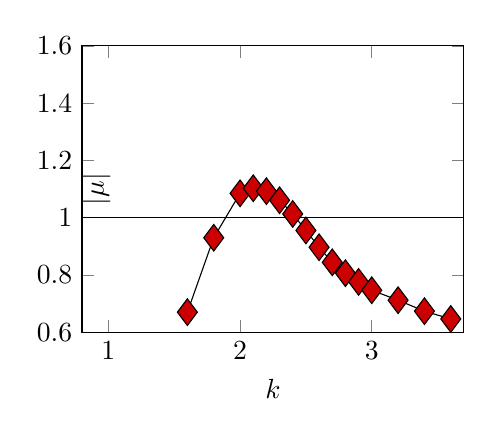
\begin{tikzpicture}



\begin{axis}[%
%width=4.3cm,
%height=3.5cm,
width=0.4\textwidth,
height=0.3\textwidth,
%width=0.2\textwidth,
%height=0.2\textwidth,
scale only axis,
%grid=both,
%axis lines=middle,
xmin=0.8,
xmax=3.7,
ymin=0.6,
ymax=1.6,
%xtick={2, 3, 4, 5, 6, 7, 8, 9, 10, 11},
%ytick={2, 2.5, 3, 3.5, 4, 4.5, 5, 5.5, 6, 6.5, 7},
%xlabel style={font=\color{white!15!black}},
xlabel={$k$},
ylabel={$|\mu|$},
ylabel style={at={(0.1,0.5)}},
%ymin=0,
%ymax=200,
axis background/.style={fill=white},
legend style={at={(0.99,0.85)}, anchor=east, legend cell align=left, align=left, fill=none, draw=none}
]


\addplot [color=black,solid,mark=diamond*,mark options={scale=2.4,black,fill=red!80!black}]
  table[row sep=crcr]{%
   %1.000000000000000   1.000070000000000 \\
  % 1.300000000000000   0.714343000000000 \\
   1.600000000000000   0.670046000000000 \\
   1.800000000000000   0.929885000000000 \\
   2.000000000000000   1.085060000000000 \\
   2.100000000000000   1.102700000000000 \\
   2.200000000000000   1.092560000000000 \\
   2.300000000000000   1.060710000000000 \\
   2.400000000000000   1.012990000000000 \\
   2.500000000000000   0.955412000000000 \\
   2.600000000000000   0.896718000000000 \\
   2.700000000000000   0.844065000000000 \\
   2.800000000000000   0.806200000000000 \\ 
   2.900000000000000   0.775755000000000 \\ 
   3.000000000000000   0.746579000000000 \\
   3.200000000000000   0.711819000000000 \\
   3.400000000000000   0.673520000000000 \\
   3.600000000000000   0.646376000000000 \\
   %4.000000000000000   0.562545000000000 \\
   %4.800000000000000   0.530527000000000 \\
   %5.000000000000000   0.524629000000000 \\
   %5.400000000000000   0.489231000000000 \\
   %5.800000000000000   0.468024000000000 \\
   %6.200000000000000   0.448075000000000 \\
};
%\addlegendentry{$Re=500$}

\addplot [color=black,solid,mark=,mark options={scale=1.4,black,fill=green!80!black}]
  table[row sep=crcr]{%
  0 1 \\
  5 1 \\
};





\end{axis}

\end{tikzpicture}%

%  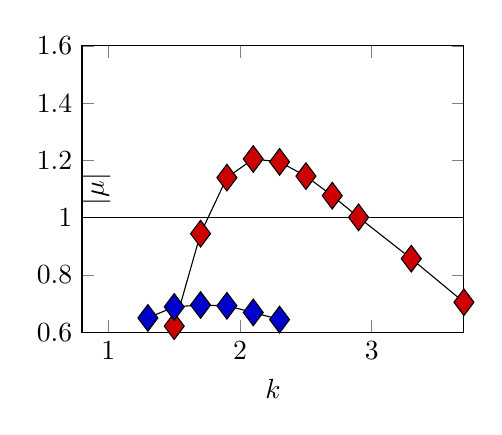
\begin{tikzpicture}



\begin{axis}[%
%width=4.3cm,
%height=3.5cm,
width=0.4\textwidth,
height=0.3\textwidth,
%width=0.2\textwidth,
%height=0.2\textwidth,
scale only axis,
%grid=both,
%axis lines=middle,
xmin=0.8,
xmax=3.7,
ymin=0.6,
ymax=1.6,
%xtick={2, 3, 4, 5, 6, 7, 8, 9, 10, 11},
%ytick={2, 2.5, 3, 3.5, 4, 4.5, 5, 5.5, 6, 6.5, 7},
%xlabel style={font=\color{white!15!black}},
xlabel={$k$},
ylabel={$|\mu|$},
ylabel style={at={(0.1,0.5)}},
%ymin=0,
%ymax=200,
axis background/.style={fill=white},
legend style={at={(0.99,0.85)}, anchor=east, legend cell align=left, align=left, fill=none, draw=none}
]


\addplot [color=black,solid,mark=diamond*,mark options={scale=2.4,black,fill=red!80!black}]
  table[row sep=crcr]{%
1.5 0.621431 \\
1.7 0.944234 \\
1.9 1.13979 \\
2.1 1.20487 \\
2.3 1.19477 \\
2.5 1.14503 \\
2.7 1.07689 \\
2.9 1.00122 \\
3.3 0.856827 \\
3.7 0.704753 \\
};
\addplot [color=black,solid,mark=diamond*,mark options={scale=2.4,black,fill=blue!80!black}]
  table[row sep=crcr]{%
1.3 0.650088 \\
1.5 0.688449 \\
1.7 0.695007 \\
1.9 0.692386 \\
2.1 0.669215 \\
2.3 0.644222 \\
};


%\addlegendentry{$Re=500$}

\addplot [color=black,solid,mark=,mark options={scale=2.4,black,fill=green!80!black}]
  table[row sep=crcr]{%
  0 1 \\
  5 1 \\
};





\end{axis}

\end{tikzpicture}%

%  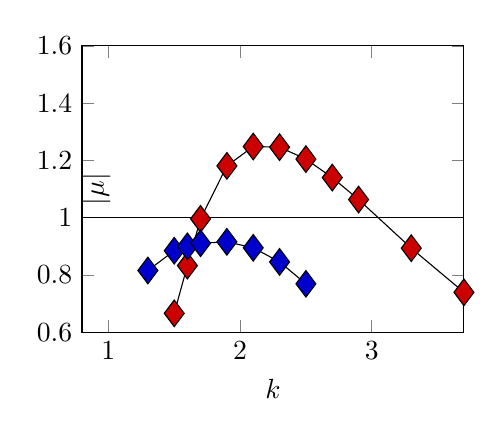
\begin{tikzpicture}



\begin{axis}[%
%width=4.3cm,
%height=3.5cm,
width=0.4\textwidth,
height=0.3\textwidth,
%width=0.2\textwidth,
%height=0.2\textwidth,
scale only axis,
%grid=both,
%axis lines=middle,
xmin=0.8,
xmax=3.7,
ymin=0.6,
ymax=1.6,
%xtick={2, 3, 4, 5, 6, 7, 8, 9, 10, 11},
%ytick={2, 2.5, 3, 3.5, 4, 4.5, 5, 5.5, 6, 6.5, 7},
%xlabel style={font=\color{white!15!black}},
xlabel={$k$},
ylabel={$|\mu|$},
ylabel style={at={(0.1,0.5)}},
%ymin=0,
%ymax=200,
axis background/.style={fill=white},
legend style={at={(0.99,0.85)}, anchor=east, legend cell align=left, align=left, fill=none, draw=none}
]


\addplot [color=black,solid,mark=diamond*,mark options={scale=2.4,black,fill=red!80!black}]
  table[row sep=crcr]{%
1.5 0.666004 \\
1.6 0.832646 \\
1.7 0.9958 \\
1.9 1.18082 \\
2.1 1.24832 \\
2.3 1.24618 \\
2.5 1.20433 \\
2.7 1.14004 \\
2.9 1.06321 \\
3.3 0.893504 \\
3.7 0.739385 \\
};
\addplot [color=black,solid,mark=diamond*,mark options={scale=2.4,black,fill=blue!80!black}]
  table[row sep=crcr]{%
1.3 0.815608 \\
1.5 0.884647 \\
1.6 0.899934 \\
1.7 0.910632 \\
1.9 0.915668 \\
2.1 0.89476 \\
2.3 0.845626 \\
2.5 0.769004 \\
%2.7 0.733247 \\
};


%\addlegendentry{$Re=500$}

\addplot [color=black,solid,mark=,mark options={scale=1.4,black,fill=green!80!black}]
  table[row sep=crcr]{%
  0 1 \\
  5 1 \\
};





\end{axis}

\end{tikzpicture}%
  
%  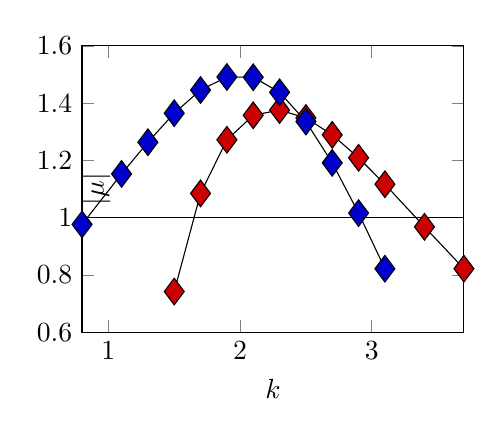
\begin{tikzpicture}



\begin{axis}[%
%width=4.3cm,
%height=3.5cm,
width=0.4\textwidth,
height=0.3\textwidth,
%width=0.2\textwidth,
%height=0.2\textwidth,
scale only axis,
%grid=both,
%axis lines=middle,
xmin=0.8,
xmax=3.7,
ymin=0.6,
ymax=1.6,
%xtick={2, 3, 4, 5, 6, 7, 8, 9, 10, 11},
%ytick={2, 2.5, 3, 3.5, 4, 4.5, 5, 5.5, 6, 6.5, 7},
%xlabel style={font=\color{white!15!black}},
xlabel={$k$},
ylabel={$|\mu|$},
ylabel style={at={(0.1,0.5)}},
%ymin=0,
%ymax=200,
axis background/.style={fill=white},
legend style={at={(0.99,0.85)}, anchor=east, legend cell align=left, align=left, fill=none, draw=none}
]


\addplot [color=black,solid,mark=diamond*,mark options={scale=2.4,black,fill=red!80!black}]
  table[row sep=crcr]{%
1.5 0.742066 \\
1.7 1.08482 \\
1.9 1.27188 \\
2.1 1.35744 \\
2.3 1.3757 \\
2.5 1.34816 \\
2.7 1.28908 \\
2.9 1.20902 \\
3.1 1.11666 \\
3.4 0.968 \\
3.7 0.821928 \\
};
\addplot [color=black,solid,mark=diamond*,mark options={scale=2.4,black,fill=blue!80!black}]
  table[row sep=crcr]{%
0.8 0.976452 \\
1.1 1.1528 \\
1.3 1.26332 \\
1.5 1.36481 \\
1.7 1.44557 \\
1.9 1.49116 \\
2.1 1.49023 \\
2.3 1.43771 \\
2.5 1.33553 \\
2.7 1.1913 \\
2.9 1.01607 \\
3.1 0.821755 \\
};


%\addlegendentry{$Re=500$}

\addplot [color=black,solid,mark=,mark options={scale=1.4,black,fill=green!80!black}]
  table[row sep=crcr]{%
  0 1 \\
  5 1 \\
};





\end{axis}

\end{tikzpicture}%

  \includegraphics[width=0.49\textwidth]{./fig/AR5s/multipliers_AR5.eps}
  \includegraphics[width=0.49\textwidth]{./fig/AR5s/multipliers_AR5p25.eps}  
  \includegraphics[width=0.49\textwidth]{./fig/AR5s/multipliers_AR5p5.eps}  
  \includegraphics[width=0.49\textwidth]{./fig/AR5s/multipliers_AR5p75.eps}      
  \vspace{0.1cm}
  \begin{tikzpicture}
  \draw (-10,2) -- (8,2);
  \end{tikzpicture}
  \vspace{0.1cm}
  \includegraphics[width=0.32\textwidth]{./fig/AR5s/Floqetmode_beta_2_Re550_AR5p5_A.png}
  \includegraphics[width=0.32\textwidth]{./fig/AR5s/Floqetmode_beta_2_Re550_AR5p5_QS.png} 
  \includegraphics[width=0.32\textwidth]{./fig/AR5s/Floqetmode_beta_4p75_Re550_AR5p5_Ap.png}
  \vspace{0.1cm}
  \begin{tikzpicture}
  \draw (-10,2) -- (8,2);
  \end{tikzpicture}
  \vspace{0.1cm}
  \includegraphics[width=0.49\textwidth]{./fig/AR5s/lambda2-AR55-Re450-3D.png}   
  \includegraphics[width=0.49\textwidth]{./fig/AR5s/lambda2-AR55-Re500-3D.png}     
  \caption{Top: Floquet multipliers for $\AR=5$ (top left), $\AR=5.25$ (top right), $\AR=5.5$ (bottom left) and $\AR=5.75$ (bottom right). The red symbols refer to mode $QS$. The blue symbols refer to mode $A$. The green symbols refer to mode $B$. Different symbols refer to different $Re$. Centre: Floquet modes associated with mode A (left), mode QS (centre) and mode $A'$ for $\AR=5.5$ and $Re=550$. Bottom: Results from the 3D DNS for $\AR=5.5$. Left: $Re=450$, right: $Re=500$. It is thus clear that mode A dominates at smaller $Re$, while once mode $QS$ becomes unstable it dominates. Mode $A'$ has the same symmetries of mode $A$ and is a synchronous mode. The difference is that its characteristic wavelength is much smaller, with $\beta_c \approx 4.5$. XX CHECK MODE GREEN FOR $AR=5.5$ and $Re=600$. POTREBBE ESSERE CHE SONO DUE MODI SEPARATI? XX}
  \label{fig:mult_AR5s}
\end{figure} 

%\section{Bodies with $6 \le \AR \le 8$}

\begin{itemize}
  \item For these $\AR$, the secondary flow instability is due to mode $QS$ that leads to a three-dimensional state. Interestingly, for these $\AR$ mode $A$ is not detected. This is consistent with the fact that for this range of $\AR$, at the intermediate $Re$, the flow is driven by the LE vortex shedding, that modifies the flow dynamics in the near-wake region where the triggering mechanism of mode $A$ takes place. 
\end{itemize}

\begin{figure}
  \centering
  \includegraphics[width=0.49\textwidth]{./fig/AR7s/multipliers_AR6.eps}  
  \includegraphics[width=0.49\textwidth]{./fig/AR7s/multipliers_AR7.eps}
  \includegraphics[width=0.49\textwidth]{./fig/AR7s/multipliers_AR7_b.eps}
  \includegraphics[width=0.7\textwidth]{./fig/AR7s/Floqetmode_beta_2p2_Re500_AR7.png}
  \caption{Floquet stability analysis for $\AR=6$ and $\AR=7$. Top: Floquet multipliers associated with the unstable branch. for $\AR=6$ (left) and $\AR=7$ (right). Centre: dependence of the real and imaginary parts of $\mu$ on $\beta$ for $\AR=7$. Bottom: three-dimensional reconstruction of the unstable Floquet mode for $\AR=7$. For these $\AR$s the secondary instability of the flow is due mode $QS$.}
  \label{fig:mult_AR7s}
\end{figure}

%\section{$\AR=9$}

\begin{figure}
  \centering
  \includegraphics[width=0.49\textwidth]{./fig/AR9s/Floquet_AR9_Re400_beta1p2_modeA.png}  
  \includegraphics[width=0.49\textwidth]{./fig/AR9s/Floquet_AR9_Re450_beta2_modeQS.png}
  \caption{Reconstruction of the Floquet modes for $\AR=9$. Left: mode $A$, $Re=400$, $\beta=1.2$. Right: mode $QS$, $Re=450$, $\beta=2$.}
  \label{fig:mult_AR9s}
\end{figure}

\begin{figure}
  \centering
  \includegraphics[width=0.49\textwidth]{./fig/AR5p5/sens_1-200-1p25_5p5-500-2_modeA_75.png}
  \includegraphics[width=0.49\textwidth]{./fig/AR5p5/sens_1-200-1p25_5p5-500-2_modeA_100.png}
  \caption{Structural sensitivity for mode A at two different instants within the shedding period. Comparison between $\AR=5.5$ at $Re=500$ and $\beta=2$ and $\AR=1$ at $Re=200$ and $\beta=1.25$. For $\AR=5.5$ the base flow is governed by the TE vortex shedding. Though, the characteristic lengths of the wake vortex are rather different the topology of the structural sensitivity resembles in both cases at the two phases. This further suggests that in both cases the two unstable modes coincide.}
  \label{fig:sens_modeA}
\end{figure}  

%\subsection{On the mehcanism of modes $A'$ and $QS$}

\begin{figure}
  \centering
  \includegraphics[width=0.49\textwidth]{./fig/LagTrac/part_AR1_Re200.eps}
  \includegraphics[width=0.49\textwidth]{./fig/LagTrac/part_AR4p5_Re410.eps}
  \includegraphics[width=0.49\textwidth]{./fig/LagTrac/part_AR5p75_Re550.eps}
  \includegraphics[width=0.49\textwidth]{./fig/LagTrac/part_AR7_Re500.eps}  
  \caption{XX AUMENTARE IL RANGE INVESTIGATO XX. PER AR=1 DOBBIAMO INVESTIGARE QUELLO CHE ABBIAMO ANCHE SOPRA AL RETTANGOLO XX}
  \label{fig:part_res}
\end{figure}    

\begin{figure}
  \centering
  \includegraphics[width=0.49\textwidth]{./fig/LagTrac/orb_AR4p5_Re410.eps}   
  \includegraphics[width=0.49\textwidth]{./fig/LagTrac/orb_AR4p5_Re410.eps} 
  \includegraphics[width=0.49\textwidth]{./fig/LagTrac/orb_AR5p75_Re550.eps}
  \includegraphics[width=0.49\textwidth]{./fig/LagTrac/orb_AR7_Re500.eps}
  \caption{XX AUMENTARE IL RANGE INVESTIGATO XX}
  \label{fig:part_res}
\end{figure}

XX POSSIAMO FARE ENDOGENEITY PER STUDIARE LA SCIA STORTA CHE VEDIAMO PER $\AR=4.5$ QUANDO SI STABILIZZA? POSSIAMO VEDERE CHI NE DETERMINA LA FREQUENZA XX

\begin{figure}
  \centering
  \includegraphics[width=0.49\textwidth]{./fig/AR5s/Ener_AR5p5_Re450_Re550_beta2.png}
  \includegraphics[width=0.49\textwidth]{./fig/AR5s/Prod_AR5p5_Re450_Re550_beta2.png}
  \includegraphics[width=0.49\textwidth]{./fig/AR5s/Trsp_AR5p5_Re450_Re550_beta2.png}
  \includegraphics[width=0.49\textwidth]{./fig/AR5s/Diss_AR5p5_Re450_Re550_beta2.png}
  \caption{Budget of energy for mode $A'$ (top) and mode $QS$ (bottom). $\AR=5.5$ and $Re=450$ (for mode $A'$) and $Re=550$ (for mode $QS$). Top left: $u_i u_i^*$. Top right: Production. Bottom left: Transport. Bottom right: Dissipation. XX DIVIDERE I COMPONENTI DEL TRASPORTO XX XX GUARDARE NELLE DIVERSE ZONE DA COSA VIENE LA CRESCITA. CI SONO DEI TERMINI CHE POSSONO AMPLIFICARE IL MODO (PROD) E ALTRI CHE LO POSSONO LOCALMENTE INVECE DAMPARE, TIPO LA CONVEZIONE. PUò PROBABILMENTE AVERE SENSO ANCHE GUARDARE I CONTRIBUTI DEI TERMINI IN MODO SEPARATO. SIA PER LE COMPONENTI CHE PER QUANTO RIGUARDA INVECE I DIVERSI TEMRINI DI TRASPORTO. GUARDA MARQUET LEFSHATS PER ENDOGENEITY. NON E' LA STESSA COSA, MA SI POSSONO FARE DEI COMMENTI ANALOGHI. POSSIAMO CALCOLARE ENDOGENEITY PER IL CICLO LIMITE? GUARDARE DOVE LA CRESCITà E' LEGATA PIU AD UN FENOMENO DI PRODUZIONE LOCALE O DI ROBA CNVETTIVA XX. PLOTTA SOPRA IL FLUSSO BASE. POSSIAMO ANCHE VEDERE EFFETTO DEL RE. FARE STESSA FIGURA AL VARIARE DEL RE IN MODO QUANTITATIVO. VEDI FIG 8 DI MAEQUT}
  \label{fig:budget_ener}
\end{figure}


\begin{figure}
  \centering
  \includegraphics[width=0.49\textwidth]{./fig/AR5s/Enst_AR5p5_Re450_Re550_beta2.png}
  \includegraphics[width=0.49\textwidth]{./fig/AR5s/ProdEnst_AR5p5_Re450_Re550_beta2.png}
  \includegraphics[width=0.49\textwidth]{./fig/AR5s/DissEnst_AR5p5_Re450_Re550_beta2.png}    
  \caption{Budget of enstrophy for mode $A'$ (top) and mode $QS$ (bottom). $\AR=5.5$ and $Re=450$ (for mode $A'$) and $Re=550$ (for mode $QS$). Top left: $\hat{\omega}_i \hat{\omega}_i^*$. Top right: Production. Bottom: Dissipation.}
  \label{fig:budget_enst}
\end{figure}  
  
%\section{Three-dimensional wake transition }
 
This section describes 3-D wake transition process and mode interactions at different Reynolds number and for different aspect ratios. To this aim, we performed direct numerical simulation XXX DettaigliXXX. The initial condition has a slight effect in determining the exact onset for the instability of modes \cite{jiang-cheng-an-2018}. In this specific case, we started from a 2D solution obtained with a potential solution of the flow, and we initially triggered a disturb of the type XXX. 

\subsection{$\AR=1.5$}



Our study started from the smaller aspect ration, $\AR=1.5$. From the Floquet instability analysis of \S \ref{sec:short}, at $Re=200$ the flow becomes unstable due to mode A. For this reason, we performed simulations from $Re=170$ to $Re=250$, with a gap of $\Delta Re=20$.XXX COMPLETE ONCE \S \ref{sec:short} HAS MORE DETAILS AND WE ARE SUREXXX. For each dataset, we computed the streamwise vorticity $\omega_x$ which has been used to characterize the wake. The two dimensional von Kármán wake persist until $Re=210$. From $Re \leq 210$ the wake undergoes a secondary instability leading to a three-dimensional state.

\begin{figure}
  \centering
  \includegraphics[trim={12cm 0 12cm 0},clip,width=0.32\textwidth]{./fig/Wake/AR1.5Re210.png}   
  \includegraphics[trim={12cm 0 12cm 0},clip,width=0.32\textwidth]{./fig/Wake/AR1.5Re230.png} 
  \includegraphics[trim={12cm 0 12cm 0},clip,width=0.32\textwidth]{./fig/Wake/AR1.5Re250.png}
  \caption{Isocontours of $\omega_x$ of the three dimensinal wake for $Re=210$ (left panel), $Re=230$  (central panel), $Re=250$ (right panel).}
  \label{fig:wake1.5}
\end{figure}  

 Figure \ref{fig:wake1.5} shows instantaneous $\omega_x=XXX$ isocontours for $Re=210$, $Re=230$, and $Re=250$. At the lowest Reynolds number, the instability is due to mode A.




\section{Conclusions}
XX CONCLUSIONS XX  



\section*{Funding} 
This research received no specific grant from any funding agency, commercial or not-for-profit sectors.

\section*{Declaration of Interests} 
The authors report no conflict of interest.


\bibliographystyle{jfm}
\bibliography{Stability}


\end{document}



